\documentclass[12pt, a4paper, oneside]{report}

\usepackage{fontspec}
\setmainfont[Script=Greek]{GFS Didot}
%\newfontfamily\greekfont[Script=Greek]{GFS Didot}
\newfontfamily{\greekfonttt}{Linux Libertine Mono}
\newfontfamily\englishfont{Linux Libertine}
\usepackage{polyglossia}

\setdefaultlanguage{greek}
\setotherlanguage{english}
%\setmainfont[Script=Greek]{GFS Didot}

%%%%%%%%%%%%%%%%%%%%%%%   Biblatex implementation//De doulevei...k omws    %%%%%%%%%%%%%%
%\usepackage[backend=biber,sortlocale=auto]{biblatex}
%\addbibresource{refs}
%\usepackage{csquotes}
%\usepackage{xpatch}

\usepackage[official]{eurosym}
\usepackage[version=4]{mhchem} %Chemical symbols
\usepackage{enumitem} %Arithmoi kai grammata stis listes
\usepackage{latexsym}
\usepackage{amsmath} %Equations
\usepackage{amsthm,amssymb}
\usepackage{wasysym}
\usepackage{booktabs}
\usepackage{ctable}
\usepackage{url} %Links sth vivliografia
\usepackage{xcolor, graphicx} %Images
\graphicspath{ {images/} }
\usepackage{tocbibind} %%Vivliografia, kat. sxhmatwn kai pinakwn sta periexomena
\usepackage{listings,color}
\definecolor{verbgray}{gray}{0.9}

%%%%%% Custom enumerate environment gia range sta items %%%%%%%%%%
\def\itemrange#1{%
\addtocounter{enumi}{1}%
\edef\labelenumi{\theenumi--\noexpand\theenumi.}%
\addtocounter{enumi}{-1}%
\addtocounter{enumi}{#1}%
\item
\def\labelenumi{\theenumi.}}

\lstnewenvironment{code}{%
  \lstset{backgroundcolor=\color{verbgray},
  frame=single,
  framerule=0pt,
  basicstyle=\ttfamily,
  columns=fullflexible,
  breaklines=true}}{}

\definecolor{shadecolor}{rgb}{.9, .9, .9}

%\usepackage{verbatim}
\usepackage{array}
\newcolumntype{L}[1]{>{\raggedright\let\newline\\\arraybackslash\hspace{0pt}}m{#1}}
\newcolumntype{C}[1]{>{\centering\let\newline\\\arraybackslash\hspace{0pt}}m{#1}}
\newcolumntype{R}[1]{>{\raggedleft\let\newline\\\arraybackslash\hspace{0pt}}m{#1}}



\title{Έξυπνα Δίκτυα Ενέργειας}

\author{Ζαππής Σωκράτης}
\date{Μάιος 2015}

\begin{document}
%%%%%%%%%%%%%%%%%%%%%%%  ARXH PROTYPOU %%%%%%%%%%%%%%%%%%%%%%
\pagenumbering{gobble}

\begin{figure}[t]
\begin{tabular}{ L{0.65\textwidth} R{0.31\textwidth }}
\textbf{{\large ΠΑΝΕΠΙΣΤΗΜΙΟ ΠΑΤΡΩΝ}\newline ΤΜΗΜΑ ΗΛΕΚΤΡΟΛΟΓΩΝ ΜΗΧΑΝΙΚΩΝ\newline ΚΑΙ ΤΕΧΝΟΛΟΓΙΑΣ ΥΠΟΛΟΓΙΣΤΩΝ\newline{\small ΤΟΜΕΑΣ:\mbox{ ΗΛΕΚΤΡΟΝΙΚΗΣ ΚΑΙ ΥΠΟΛΟΓΙΣΤΩΝ}}}\newline {\footnotesize ΕΡΓΑΣΤΗΡΙΟ ΣΥΣΤΗΜΑΤΩΝ ΥΠΟΛΟΓΙΣΤΩΝ}
&

\includegraphics[scale=0.3]{uni_logo}  \\
\bottomrule
\end{tabular}
\end{figure}

\begin{center}
{\large
\vspace*{2ex}
{\Large\textbf{Διπλωματική Εργασία}}\\του φοιτητή του Τμήματος Ηλεκτρολόγων Μηχανικών και\\Τεχνολογίας Υπολογιστών της Πολυτεχνικής Σχολής του\\Πανεπιστημίου Πατρών
\vskip 1cm
Ζαππή Σωκράτη του Σπυρίδωνα\vskip 2ex
Αριθμός Μητρώου:~5966 \vskip 3ex
\underline{\smash{Θέμα}}\vskip 2ex {\Large\textbf{<<Έξυπνα Δίκτυα Ενέργειας>>}}
\vskip 1cm \underline{\smash{Επιβλέπων}}\vskip 2ex Χούσος Ευθύμιος \vskip 6ex 
\textbf{Αριθμός Διπλωματικής Εργασίας:}\\  
\vskip 7ex
Πάτρα, Μάιος 2015
}
%\end{center}
%\rule{\textwidth}{1.5pt}
\clearpage
%\begin{center}
{\large
{\Large\textbf{ΠΙΣΤΟΠΟΙΗΣΗ}} \vskip 2ex Πιστοποιείται ότι η Διπλωματική Εργασία με θέμα \vskip 2ex \textbf{{\large<<Έξυπνα Δίκτυα Ενέργειας>>}} \vskip 3ex
Του φοιτητή του Τμήματος Ηλεκτρολόγων Μηχανικών και Τεχνολογίας Υπολογιστών \vskip 3ex Σωκράτη Ζαππή του Σπυρίδωνα \vskip 2ex Αριθμός Μητρώου: 5966 \vskip 5ex Παρουσιάστηκε δημόσια και εξετάστηκε στο Τμήμα Ηλεκτρολόγων Μηχανικών και Τεχνολογίας Υπολογιστών στις\\........./........./.........
\vskip 2cm}

\begin{figure}[b]
\centering
\begin{tabular}{ L{0.5\textwidth} R{0.5\textwidth}}
Ο Επιβλέπων & Ο Διευθυντής του Τομέα \\
 & \\
 & \\
Χούσος Ευθύμιος & Χούσος Ευθύμιος\\
Καθηγητής & Καθηγητής\\
\end{tabular}
\end{figure}
\end{center}
\clearpage
\begin{flushleft}
{\large\textbf{Αριθμός Διπλωματικής Εργασίας: \vskip 4ex Θέμα:~<<Έξυπνα Δίκτυα Ενέργειας>> \vskip 4ex}
\begin{tabular}{L{3cm} R{6cm}}
Φοιτητής: & Ζαππής Σωκράτης\\
Επιβλέπων: & Χούσος Ευθύμιος\\
\end{tabular}
}
\end{flushleft}
%%%%%%%%%%%%%%%%%%%%%%%%%  TELOS PROTYPOU %%%%%%%%%%%%%%%%%%%%%%
\clearpage

\maketitle
\clearpage
\pagenumbering{roman}
\setcounter{page}{2}
\section*{Περίληψη}
Σκοπός της παρούσας διπλωματικής ήταν να μπορέσουμε να δώσουμε πρόσβαση στο διαδίκτυο μέσω δικτύου κινητής τηλεφωνίας, σε μια συσκευή BeagleBone η οποία ελέγχει μετρητές ενέργειας μέσω δικτύου ZigBee. Το όλο πακέτο με τις συσκευές μέτρησης, το BeagleBone και τον coordinator που επικοινωνεί με τις μετρητικές συσκευές, παράγεται από την εταιρεία Meazon στην οποία έκανα την πρακτική μου άσκηση. Σχεδιάστηκε από μηχανικούς της Meazon μια PCB πλακέτα που έχει ένα GPRS module της εταιρείας u-blox, η οποία προσαρτάται στο BeagleBone, δίνοντάς του έτσι τη δυνατότητα σύνδεσης στο διαδίκτυο. Αντικείμενο της διπλωματικής ήταν να γράψουμε τους απαραίτητους drivers ώστε να λειτουργήσει το module σωστά με το BeagleBone, έτσι ώστε να το μετατρέψουμε σε ένα GPRS modem ώστε να μπορούμε να ελέγχουμε τις μετρητικές συσκευές μέσω διαδικτύου, καθώς και για να μεταφέρονται οι μετρήσεις των συσκευών στο cloud της Meazon.

Στην αρχή του πρώτου κεφαλαίου γίνεται μια περιγραφή των τρέχοντων ηλεκτρικών δικτύων. Μετά ακολουθεί μια εισαγωγή στα έξυπνα δίκτυα, με περιγραφή των χαρακτηριστικών τους καθώς και μια προσπάθεια για τον ορισμό ενός έξυπνου δικτύου. Περιγράφονται επίσης οι προκλήσεις που θα κληθούν να αντιμετωπίσουν τα έξυπνα δίκτυα.

Στο δεύτερο κεφάλαιο παρουσιάζεται η επικοινωνία μεταξύ μηχανών (Machine to Machine - M2M) και τα κυριότερα στοιχεία της, όπως και οι τομείς στους οποίους βρίσκει εφαρμογή.

Στο τρίτο κεφάλαιο παρουσιάζεται η έννοια του Διαδικτύου των Πραγμάτων (Internet of Things), οι τεχνολογίες που αυτό υιοθετεί, η γενικότερη αρχιτεκτονική του, καθώς και οι εφαρμογές που λαμβάνει μέρος.

Στο τέταρτο και πέμπτο κεφάλαιο γίνεται μια περιγραφή των μετρητικών συσκευών που κατασκευάζει η Meazon Α.Ε., το BeagleBone το οποίο χρησιμοποιείται για τον έλεγχό τους και επίσης γίνεται περιγραφή του πρωτοκόλλου ZigBee που αυτές χρησιμοποιούν για τη μεταξύ τους επικοινωνία, καθώς και οι λόγοι για τους οποίους προτιμήθηκε αυτό το πρωτόκολλο έναντι των εναλλακτικών. Ακόμα, κάνουμε μια σύντομη παρουσίαση  των αντίστοιχων πλατφορμών που υπάρχουν στο εμπόριο, τις συγκρίνουμε με το BeagleBone και παραθέτουμε τους λόγους που οδήγησαν τελικά στην επιλογή του.

Στο έκτο και τελευταίο κεφάλαιο, δείχνουμε τα βήματα που ακολουθήθηκαν για να δώσουμε τη δυνατότητα στο BeagleBone να συνδεθεί στο διαδίκτυο μέσω GPRS με τη χρήση της πλακέτας επέκτασης που σχεδιάστηκε στη Meazon. Δείχνουμε επίσης τι χρειάστηκε να κάνουμε για να μπορέσουμε να χρησιμοποιήσουμε το real time clock της πλακέτας. Τέλος, παραθέτουμε κάποια παραδείγματα όπου θα μπορούσε να βρει εφαρμογή η πλατφόρμα με την πλακέτα επέκτασης.

\clearpage
\section*{\textenglish{Abstract}}
\begin{english}The purpose of this thesis was managing to give access to the internet through the mobile telephony network, to a BeagleBone device which controls energy metering devices through a ZigBee network. The whole bundle consisting of the metering devices, the BeagleBone and the coordinator which communicates with the metering devices, is produced by the company Meazon, where I carried out my internship. The engineers at Meazon designed a printed circuit expansion board that has a GPRS module on it, produced by a company called u-blox, and the board is attached to the BeagleBone, giving it the ability to connect to the internet. The objective of this thesis was to write the necessary drivers in order for the module to work properly with the BeagleBone, so that we could make the BeagleBone act as a GPRS modem and be able to control the metering devices remotely through the internet, as well as giving the metering devices the ability to send their metering data to Meazon's cloud.

In the beginning of the f\mbox{}irst chapter, we have a description of the current energy grids. After that, follows a general introduction to the Smart Grid, with a description of its main characteristics as well as an attempt to def\mbox{}ine the Smart Grid. The challenges that the smart grids are bound to come up against are also addressed.

In the second chapter we present the Machine to Machine communication (M2M) and its main elements, as well as the areas that this technology can be applied.

In the third chapter we present the concept of the Internet of Things (IoT), the technologies it comprises, its general architecture and the applications it takes place in.

In the fourth and f\mbox{}ifth chapter we describe the metering devices that are produced by Meazon S.A., the BeagleBone platform which is used for their control and we also describe the ZigBee protocol they use for communicating with each other. Furthermore, we list the reasons which led to the use of this protocol instead of the other available alternatives. Lastly, we make a short presentation of other similar platforms available on the market, we compare them against the BeagleBone and present the causes that contributed to it being our platform of choice.

In the sixth and f\mbox{}inal chapter, we show the steps we followed in order to give BeagleBone the ability to connect to the internet through GPRS, with use of the expansion board that was designed and produced by Meazon. We also show what needs to be done so that we are able to use the board's real time clock. Finally, we present some examples where the platform including the expansion board could f\mbox{}ind application.
\end{english}
\clearpage

\section*{Ευχαριστίες}
Η παρούσα διπλωματική εκπονήθηκε στο τμήμα Ηλεκτρολόγων Μηχανικών και Τεχνολογίας Υπολογιστών του Πανεπιστημίου Πατρών. Για την εκπόνηση αυτής, θα ήθελα να ευχαριστήσω πρώτα τον επιβλέποντα καθηγητή μου, κ. Χούσο Ευθύμιο, για την ευκαιρία που μου έδωσε με την ανάθεση του θέματος, την εμπιστοσύνη που μου έδειξε, καθώς και για την υπομονή και την καθοδήγησή του καθ'όλη τη διάρκεια της εργασίας αυτής.

Επίσης, θα ήθελα να ευχαριστήσω θερμά την εταιρεία Meazon Α.Ε. και ιδιαίτερα τον κ. Κουτρουμπίνα Στυλιανό, διευθύνοντα σύμβουλο και ιδρυτικό μέλος της εταιρείας, για την ευκαιρία που μου έδωσε να εργαστώ σε μια εταιρεία τεχνολογίας αιχμής, καθώς και για το συνεχές του ενδιαφέρον και τις χρήσιμες συμβουλές του. Θα ήθελα ακόμα να ευχαριστήσω τα παιδιά που γνώρισα και συνεργαστήκαμε στην εταιρεία, οι οποίοι είναι οι Νίκος, Παναγιώτης, Πέτρος και Τίτος,  η βοήθεια των οποίων έπαιξε πολύ σημαντικό ρόλο στην εργασία αυτή.

Τέλος, θέλω να ευχαριστήσω την οικογένεια και τους φίλους μου για τη στήριξη και τη συμπαράσταση που μου έδειχναν σε όλη τη διάρκεια των σπουδών μου.

\clearpage

\tableofcontents
\listoffigures
\listoftables
\clearpage
\phantom{mpl}
\clearpage
\pagenumbering{arabic}
\chapter{Εισαγωγή στα Έξυπνα Δίκτυα - Smart Grids}

\section{Τα ηλεκτρικά Δίκτυα σήμερα}

Ο ηλεκτρισμός είναι ένα αναπόσπαστο κομμάτι της ζωής μας. Τόσο άρρηκτα συνδεδεμένο με κάθε τομέα της ανθρώπινης δραστηριότητας που δε θα ήταν υπερβολή να πούμε πως είναι η κινητήριος δύναμη ολόκληρου του κόσμου και ο ουσιαστικότερος φορέας εξέλιξης και προόδου σήμερα. Από τον Nicola Tesla ο οποίος παρουσίασε στις 16 Μαΐου του 1888 στο Αμερικανικό Ινστιτούτο Ηλεκτρομηχανικής μια πρωτοποριακή ιδέα για <<το Νέο Σύστημα Κινητήρων και Μετασχηματισμών Εναλλασσόμενου Ρεύματος>>, μέχρι τις αρχές του 20ου αιώνα και τη δημιουργία των πρώτων ηλεκτρικών δικτύων μεταφοράς ρεύματος τα οποία χαρακτηρίστηκαν ως το σπουδαιότερο επίτευγμα του αιώνα από την Εθνική Ακαδημία Μηχανικών (National Academy of Engineers), αλλά και μέχρι τις μέρες μας, ο ηλεκτρισμός εξακολουθεί να αλλάζει σημαντικά τη ζωή μας.

Στην ουσία ένα ηλεκτρικό δίκτυο σήμερα καθιστά εφικτή την παραγωγή , μεταφορά και διανομή ηλεκτρικής ενέργειας από τον σταθμό παραγωγής στον καταναλωτή \cite{4}. Ένα τυπικό ηλεκτρικό δίκτυο \cite{6}, αποτελείται από ηλεκτροπαραγωγούς σταθμούς (power plants), υποσταθμούς μεταφοράς ανύψωσης τάσης (step-up transmission substations), υποσταθμούς μεταφοράς υψηλής τάσης και υποβιβασμού της σε μέση τάση (step-down transmission substations), υποσταθμούς διανομής μέσης τάσης και υποβιβασμού σε χαμηλή τάση (distribution substations) και γραμμές διανομής υψηλής, μέσης και χαμηλής τάσης (transmission and distribution lines). Η ενέργεια η οποία παράγεται στους ηλεκτροπαραγωγούς σταθμούς προέρχεται από ανανεώσιμες ή μη, πηγές ενέργειας. Οι ανανεώσιμες πηγές ενέργειας κατατάσσονται συνήθως σε δύο κατηγορίες: τις μεταβλητές~(ηλιακή, αιολική ενέργεια) και τις μη μεταβλητές πηγές ενέργειας~(υδροηλεκτρική, βιομάζα, γεωθερμική ενέργεια). Οι μη ανανεώσιμες (και μη μεταβλητές) πηγές ενέργειας αφορούν συνήθως στα ορυκτά καύσιμα (κάρβουνο, πετρέλαιο, φυσικό αέριο) ή την πυρηνική ενέργεια~\cite{6}. Όπως και να παράγεται όμως η ενέργεια στους ηλεκτροπαραγωγούς σταθμούς, το επόμενο βήμα είναι το ίδιο και έχει να κάνει με τη μεταφορά της μέσω μετασχηματιστών σε υψηλές τάσεις, πριν από την εισαγωγή της στο δίκτυο μεταφοράς, ώστε να ελαχιστοποιηθούν οι απώλειες λόγω του φαινομένου του Joule. Μέσω των γραμμών μεταφοράς υψηλής τάσης η ενέργεια αυτή φτάνει σε υποσταθμούς μεταφοράς η οποίοι μετασχηματίζουν την υψηλή τάση σε μέση τάση για να συνεχίσει να μεταφέρεται μέσω των γραμμών μεταφοράς προς τους υποσταθμούς διανομής οι οποίοι μετασχηματίζοντας τη μέση τάση σε χαμηλή, παραδίδουν πλέον την ενέργεια σε γραμμές διανομής χαμηλής τάσης οι οποίες συνδέονται με τα υποστατικά μας. Το Σχ.~\ref{eik0} αποτελεί την αναπαράσταση της συγκεκριμένης διαδικασίας.
\begin{figure}[!h]
\centering
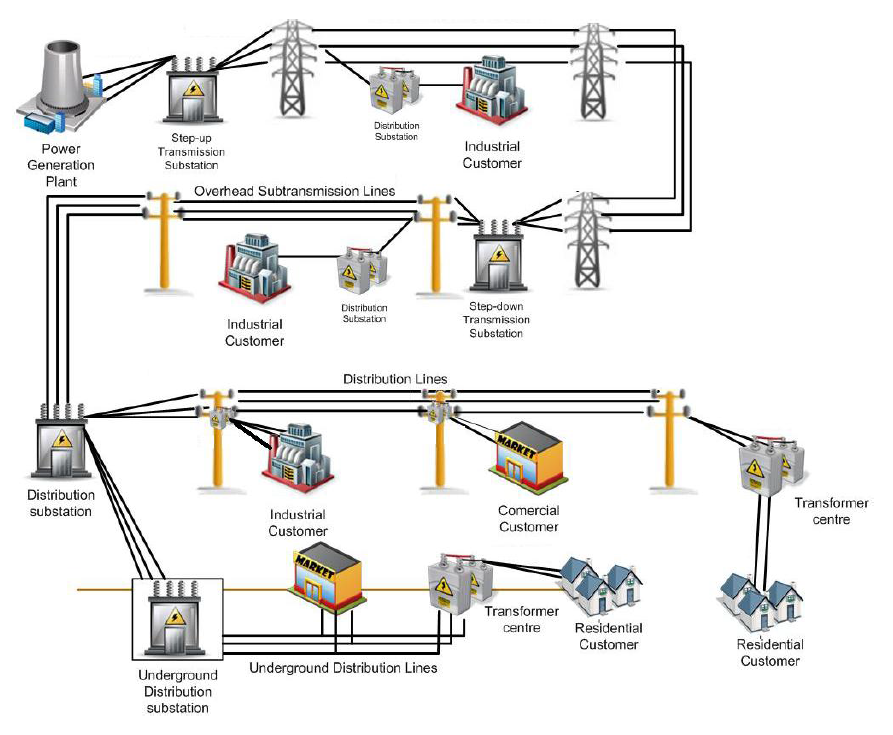
\includegraphics[scale=0.496]{eikona_00}
\caption[Η μεταφορά και διάδοση της ηλεκτρικής ενέργειας από την παραγωγή στην κατανάλωση]{Η μεταφορά και διάδοση της ηλεκτρικής ενέργειας από την παραγωγή στην κατανάλωση\cite{6}}\label{eik0}
\end{figure}

Οι υποσταθμοί μεταφοράς ηλεκτρικής ενέργειας βέβαια πέρα από το ρόλο που διαδραματίζουν για το μετασχηματισμό τάσης σχεδιάζονται στις πλείστες των περιπτώσεων με τρόπο τέτοιο που να εξασφαλίζονται διασυνδέσεις εναλλακτικής τροφοδοσίας από υφιστάμενους υποσταθμούς, σε περιπτώσεις κατά τις οποίες ένας υποσταθμός δε μπορεί να χρησιμοποιηθεί για κάποιο λόγο (π.χ. εργασίες συντήρησης), πράγμα που αυξάνει την αξιοπιστία του δικτύου μεταφοράς ηλεκτρικής ενέργειας. Παράλληλα, μέσα στους υποσταθμούς μεταφοράς εντοπίζονται μεταξύ άλλων διακόπτες κυκλωμάτων (circuit breakers) οι οποίοι αξιοποιούνται για αποσύνδεση από το σύστημα μεταφοράς (για απομόνωση των εγκαταστάσεων ή\slash και των μηχανημάτων), αλλά και μονάδες συλλογής δεδομένων του υποσταθμού για αποστολή τους σε ένα κέντρο ελέγχου ενέργειας \cite{9}.

Η μεταφορά της ηλεκτρικής ισχύος από την παραγωγή στο δίκτυο διανομής μέσω των υποσταθμών μεταφοράς είναι μια διαδικασία της οποίας τον έλεγχο αναλαμβάνει συνήθως ένας Διαχειριστής Συστήματος Μεταφοράς (Transmission System Operator – TSO). Βασικός στόχος του κάθε Διαχειριστή Συστήματος Μεταφοράς είναι μεταξύ άλλων, η εξασφάλιση της ομαλής και αποδοτικής λειτουργίας του ηλεκτρικού δικτύου. Ουσιαστικής σημασίας για την επίτευξή της, είναι η ύπαρξη των κατάλληλων συστημάτων και εξοπλισμού προκειμένου να επιτυγχάνεται η διαρκής παρακολούθηση του δικτύου για την όσο το δυνατό πιο άμεση αποκατάσταση παροχής ηλεκτρικής ενέργειας μετά από περιστατικά διακοπής και την όσο το δυνατό πιο ακριβή πρόβλεψη της ζήτησης για ισοζυγισμό της παραγωγής \cite{6}. Το βασικό σύστημα πίσω από αυτή τη διαδικασία σήμερα είναι γνωστό σαν Σύστημα Εποπτικού Ελέγχου και Συλλογής Πληροφοριών (Supervisory Control and Data Acquisition system – SCADA). Ένα τέτοιο σύστημα εκτελεί στην πραγματικότητα 4 βασικές λειτουργίες : συλλογή, επεξεργασία και παρουσίαση δεδομένων και έλεγχο του συστήματος \cite{9}. Η συλλογή δεδομένων από ολόκληρο το δίκτυο μεταφοράς καθίσταται δυνατή μέσω εξοπλισμού ο οποίος περιλαμβάνει αισθητήρες και τηλετερματικό εξοπλισμό (Remote Terminal Units – RTUs) ο οποίος μετατρέπει τα σήματα των αισθητήρων σε ψηφιακή πληροφορία, την οποία μεταφέρει στο σύστημα επεξεργασίας δεδομένων μέσω τηλεπικοινωνιακών διασυνδέσεων \cite{6,9}. Η επεξεργασία γίνεται από ένα σύνολο συστημάτων μεγάλης υπολογιστικής ισχύος τα οποία παρουσιάζουν την πληροφορία που προέκυψε από τα δεδομένα σε μια μορφή που αποκτά νόημα για τους τεχνικούς που είναι υπεύθυνοι για την παρακολούθηση του δικτύου μέσω της διεπαφής (Human Machine Interface – HMI) που διαθέτει κάθε σύστημα SCADA. Η διεπαφή αυτή, παρουσιάζει σε κατανοητή μορφή την πληροφορία που αφορά στην κατάσταση του δικτύου, δίνοντας ουσιαστικά τη δυνατότητα στον ελεγκτή της να έχει άμεση πληροφόρηση για ό,τι αφορά στο δίκτυο, τη θέση των διακοπτών , τη φόρτιση των γραμμών, τα επίπεδα τάσης, τα επίπεδα παραγωγής από όλες τις μονάδες, την κατάσταση του εξοπλισμού, τη θερμοκρασία εντός των υποσταθμών κτλ. Μέσω αυτής καθίσταται δυνατός ο εντοπισμός προβληματικών καταστάσεων οι οποίες απειλούν την ομαλή λειτουργία του ηλεκτρικού δικτύου, και οι οποίες ταξινομούνται από το σύστημα βάσει της επικινδυνότητάς τους με τις πιο σοβαρές να αξιολογούνται ως ύψιστης προτεραιότητας, πράγμα το οποίο συμβάλλει στην όσο το δυνατό πιο άμεση ανταπόκριση. Τα συστήματα αυτά παρέχουν επιπρόσθετα και τη δυνατότητα ελέγχου και τηλεχειρισμού του εξοπλισμού που βρίσκεται στους υποσταθμούς, πράγμα το οποίο σε πολλές περιπτώσεις έχει ως αποτέλεσμα την αποκατάσταση μιας βλάβης χωρίς να χρειαστεί φυσική παρουσία τεχνικού στον υποσταθμό που αντιμετώπισε το πρόβλημα.

Ένα ολοκληρωμένο σύστημα SCADA συνεργάζεται πάντα με ένα Σύστημα Διαχείρισης Ενέργειας (Energy Management System -EMS)\cite{9}. Το EMS αποτελείται στην πραγματικότητα από ένα σύνολο εφαρμογών οι οποίες έχουν ως στόχο τους τη βελτιστοποίηση της διαδικασία παραγωγής και μεταφοράς, ώστε να είναι όσο το δυνατό πιο αποδοτική, ασφαλής και οικονομική. Ένα σύστημα EMS είναι υπεύθυνο για την πρόβλεψη διακύμανσης ζήτησης ηλεκτρικής ενέργειας για την επόμενη μέρα, πρόβλεψη η οποία γίνεται εφικτή βάσει ενός ιστορικού ζήτησης ηλεκτρικής ενέργειας σε μέρες συγκρίσιμες με την αυριανή (π.χ. μέρες με τις ίδιες καιρικές συνθήκες, την ίδια εποχή, στις ίδιες ώρες). Μετά την πρόβλεψη, το σύστημα οφείλει να προχωρήσει στην εισήγηση του καλύτερου τρόπου αξιοποίησης των μονάδων παραγωγής, βάσει της πρόβλεψης ζήτησης και βάσει της πιο συμφέρουσας οικονομικά λύσης. Παράλληλα, η δυνατότητα προσομοίωσης της κατάστασης του δικτύου σε περίπτωση αποσύνδεσης εξοπλισμού προκειμένου να λαμβάνονται μέτρα πριν από προγραμματισμένες ενέργειες, εμπίπτει επίσης στις δυνατότητες ενός EMS.

\section{Οι αδυναμίες του τρέχοντος ηλεκτρικού δικτύου}

Κάπως έτσι η ηλεκτρική ενέργεια παράγεται και φτάνει στα σπίτια μας. Με μια διαδικασία η οποία ελάχιστα άλλαξε μέσα στα τελευταία 100 χρόνια~\cite{4}. Η εξέλιξη της τεχνολογίας έχει φέρει προφανώς την αυτοματοποίηση στην παραγωγή της ηλεκτρικής ενέργειας και στα συστήματα ελέγχου της, ωστόσο σε καμία περίπτωση δε μπορούμε να πούμε ότι έφερε την επανάσταση στον τομέα αυτό, όπως έχει κάνει σε τόσους άλλους τομείς της βιομηχανίας. Καθώς όμως τα χρόνια περνούν οι απαιτήσεις μας αλλάζουν, πράγμα το οποίο απαιτεί και τα συστήματά μας να μπορούν να συμβαδίζουν και να ανταποκρίνονται σε αυτές. Έχουμε πλέον αρχίσει να αντιλαμβανόμαστε τις αδυναμίες του παρόντος ηλεκτρικού δικτύου.

Προφανώς, ένα δίκτυο το οποίο λειτουργεί βασισμένο σε μεγάλους κεντρικούς ηλεκτροπαραγωγούς σταθμούς, χτισμένους σε στρατηγικά σημεία και συνδεδεμένους με συστήματα μεταφοράς υψηλής τάσης για να στηρίζουν την ηλεκτροδότηση μεγάλων περιοχών, στηρίζεται στη διακίνηση ενός τεράστιου όγκου πληροφορίας από και προς τα κέντρα παραγωγής. Αυτό έχει ως αποτέλεσμα η πληροφορία αυτή να φτάνει πολλές φορές με καθυστερήσεις στον προορισμό (high data latency), γεγονός το οποίο στερεί τη δυνατότητα στο σύστημα να διενεργεί έλεγχο σε πραγματικό χρόνο.

Την ίδια στιγμή, μια άλλη αδυναμία του τρέχοντος δικτύου ηλεκτροδότησης έγκειται στη μονόπλευρη φύση της επικοινωνίας και διανομής ενέργειας, η οποία υπαγορεύει πως ενέργεια μεταφέρεται μόνο από τον ηλεκτροπαραγωγό σταθμό στο δίκτυο και κατά συνέπεια στον πελάτη, χωρίς ο πελάτης να μπορεί να συμβάλει στη βελτίωση της αποδοτικότητας του δικτύου εισάγοντας σε αυτό δικές του πηγές ενέργειας (ηλιακή ενέργεια, αιολική ενέργεια από ιδιόκτητες εγκαταστάσεις)~\cite{11}.

Αυτή η αδυναμία του τρέχοντος ηλεκτρικού δικτύου να ενσωματώσει με επιτυχία τις εναλλακτικές πηγές ενέργειας (οι οποίες εξαρτώνται από τοπικές και καιρικές συνθήκες) στο δίκτυο, με τρόπο που να μην επηρεάζεται η αξιοπιστία του συστήματος (η οποία τώρα εξασφαλίζεται από την επεξεργασία των μη ανανεώσιμων μη μεταβλητών πηγών ενέργειας οι οποίες εγγυημένα θα δώσουν το ζητούμενο ποσοστό ηλεκτρικής ενέργειας), έχει παράλληλα και σημαντικές επιπτώσεις στο περιβάλλον, η ρύπανση του οποίου αποτελεί ένα σημαντικό πρόβλημα σήμερα~\cite{12}.

Πέραν όλων αυτών βέβαια, άλλο ένα σημαντικό μειονέκτημα του τρέχοντος ηλεκτρικού δικτύου έχει να κάνει με την αδυναμία να αποθηκεύσουμε την ηλεκτρική ισχύ με εύκολο τρόπο~\cite{13}, πράγμα το οποίο έχει ως αποτέλεσμα, προκειμένου το τρέχον δίκτυο να μπορεί να ανταποκριθεί στις απαιτήσεις της επόμενης ημέρας (χωρίς να διαθέτει απόθεμα ενέργειας), να κάνει μια πρόβλεψη για την ζήτηση ηλεκτρικής ενέργειας της επόμενης ημέρας. Παρά τις προσπάθειες για εξασφάλιση όσο το δυνατό μεγαλύτερης ακρίβειας σε αυτές τις προβλέψεις, η ζήτηση δε μπορεί ποτέ να προβλεφθεί με απόλυτη επιτυχία. Αυτό έχει πολύ συχνά ως αποτέλεσμα είτε την παραγωγή περισσότερης ενέργειας από όση πραγματικά θα χρειαστεί, με αποτέλεσμα η επιπλέον αυτή ενέργεια να μη χρησιμοποιείται πουθενά (αλλά το κόστος της παραγωγής της να επιβαρύνει τον πελάτη), είτε τη διακοπή ρεύματος (rolling blackouts) λόγω μιας κακής εκτίμησης η οποία είχε ως αποτέλεσμα την παραγωγή λιγότερης ενέργειας από αυτή που πραγματικά ζητήθηκε την επόμενη μέρα~\cite{12}.

Όλα αυτά έρχονται φυσικά να επιβαρυνθούν και από το γεγονός ότι το τρέχον σύστημα χρειάζεται τη φυσική παρέμβαση ενός χειριστή προκειμένου να μπορέσει να επανέλθει σε κατάσταση λειτουργίας κατόπιν οποιασδήποτε βλάβης \cite{15}.

Φτάσαμε λοιπόν, σε ένα σημείο όπου η αδυναμία του τρέχοντος ηλεκτρικού δικτύου να ανταποκριθεί στις ολοένα αυξανόμενες απαιτήσεις μας, δημιούργησε την ανάγκη για έναν πιο έξυπνο επανασχεδιασμό του ηλεκτρικού δικτύου του 21ου αιώνα. Στο νέο αυτό δίκτυο οι τεχνολογίες της επικοινωνίας και της πληροφορίας θα διαδραματίζουν κεντρικό ρόλο σε όλα τα επιμέρους στάδια από την παραγωγή μέχρι την κατανάλωση. Κάπως έτσι γεννήθηκε η ιδέα του Smart Grid.

\section{Ένα έξυπνο ηλεκτρικό δίκτυο - Smart Grid}

\subsection{Ορίζοντας το Έξυπνο Δίκτυο}

Σύμφωνα με το Electric Power Research Institute (ERPI), το Έξυπνο Δίκτυο παρουσιάζεται ως <<μία ευφυής υποδομή παροχής ηλεκτρικής ενέργειας η οποία υποστηρίζεται από τις τελευταίες τεχνολογίες στον τομέα της επικοινωνίας, του υπολογισμού και της ηλεκτρονικής, προκειμένου να ανταποκριθεί στις μελλοντικές απαιτήσεις της κοινωνίας σε ηλεκτρική ενέργεια>>. Σε μια άλλη εκδοχή, το Γραφείο Μεταφοράς και Διανομής Ενέργειας του Department of Energy (DoE) των ΗΠΑ, ορίζει το Έξυπνο Δίκτυο ως τη λύση που <<θα εξασφαλίσει την αξιοπιστία, την ασφάλεια και την αποδοτικότητα του ηλεκτρικού συστήματος μέσω ανταλλαγής πληροφοριών, κατανεμημένης παραγωγής και αποθήκευσης της ενέργειας>>. Η Ευρωπαϊκή Επιτροπή, μέσω του COM(2011) 202 ``Smart Grids: from innovation to deployment'' \cite{16} παρουσιάζει το Έξυπνο Δίκτυο ως <<ένα εξελιγμένο ηλεκτρικό δίκτυο, του οποίου αναπόσπαστο κομμάτι είναι η αμφίδρομη επικοινωνία μεταξύ παραγωγού και καταναλωτή και τα ευφυή συστήματα μέτρησης και παρακολούθησης της λειτουργίας του>>. Ενώ το European Commission Task Force for Smart Grid \cite{17} ορίζει το Έξυπνο Δίκτυο ως <<ένα ηλεκτρικό δίκτυο το οποίο με αποδοτικό τρόπο μπορεί να ενσωματώσει τη συμπεριφορά και τις δράσεις όλων των παραγόντων που βρίσκονται συνδεδεμένοι σε αυτό –παραγωγοί, καταναλωτές ή και καταναλωτές που παράγουν ενέργεια – ώστε να διασφαλίσει ένα οικονομικά αποδοτικό, βιώσιμο σύστημα ενέργειας με χαμηλές απώλειες και υψηλής ποιότητας υπηρεσία, σε ένα ασφαλές και αξιόπιστο δίκτυο>>.

Από τους πιο πάνω ορισμούς μπορεί κανείς να καταλάβει πως ένα Έξυπνο Δίκτυο δεν είναι τίποτα άλλο παρά η μετεξέλιξη του τρέχοντος ηλεκτρικού δικτύου σε ένα δίκτυο στο οποίο η τεχνολογία της πληροφορίας θα έχει τον πρώτιστο ρόλο. Στην ουσία, η τεχνολογία της πληροφορίας θα επιτρέπει πλέον τον απομακρυσμένο έλεγχο όλων των σταδίων από την παραγωγή στην κατανάλωση, την αμφίδρομη επικοινωνία μεταξύ παραγωγής και κατανάλωσης (δίνοντας την ευκαιρία στον καταναλωτή να μετέχει και στην παραγωγή ως prosumer), την εξασφάλιση βιωσιμότητας (sustainability) και ποιότητας υπηρεσιών, την κατανεμημένη (distributed) παραγωγή ηλεκτρικής ενέργειας, την επεξεργασία της πληροφορίας σε τοπικό επίπεδο (χωρίς να απαιτείται αποστολή της σε ένα κεντρικό σημείο), την αποθήκευσή της παραγόμενης ενέργειας και την έξυπνη μέτρηση της κατανάλωσής της. Όλα αυτά έχοντας ως κυρίαρχο στόχο την εξασφάλιση αξιοπιστίας, αποδοτικότητας και ασφάλειας.
\begin{itemize}
\item Αξιοπιστίας μέσω του σχεδιασμού του συστήματος με τέτοιο τρόπο ώστε να μπορεί να λειτουργεί αυτοάνοσα – ανιχνεύοντας την αιτία των προβλημάτων του και διορθώνοντάς τα, βρίσκοντας παράλληλα εναλλακτικούς τρόπους τροφοδότησης σε περιπτώσεις που οι υφιστάμενοι δεν μπορούν να ανταποκριθούν στις απαιτήσεις. Κάτι τέτοιο προφανώς μειώνει και τον κίνδυνο για blackouts τα οποία έχουν σημαντικό αντίκτυπο σε οικονομικό αλλά και σε κοινωνικό επίπεδο.
\item Αποδοτικότητας, μέσω της αξιοποίησης εναλλακτικών μορφών ενέργειας για τη βελτιστοποίηση της διαδικασίας παραγωγής-μεταφοράς και διάδοσης ενέργειας αλλά και μέσω της εμπλοκής του πελάτη στη διαδικασία εξοικονόμησης ενέργειας πράγμα το οποίο μπορεί να επιτευχθεί μέσω ευέλικτων προγραμμάτων demand-response.
\item Ασφάλειας μέσω πιο προσεγμένου ελέγχου και παρακολούθησης της διαδικασίας ηλεκτροδότησης \cite{11}.
\end{itemize}

\subsection{Τα αναμενόμενα πλεονεκτήματα ενός <<Έξυπνου>> Δικτύου}

Στις 13 Σεπτεμβρίου του 2011 το Τμήμα Εμπορίου του Εθνικού Ινστιτούτου Προτύπων και Τεχνολογιών (National Institute of Standards and Technology - NIST) των ΗΠΑ και η Συντονιστική Επιτροπή Έξυπνων Δικτύων της Ευρωπαϊκής Ένωσης (Smart Grid Coordination Group - SG-CG), σε κοινή τους ανακοίνωση δήλωσαν την πρόθεσή τους να συνεργαστούν για την ανάπτυξη κοινών προτύπων για τη σχεδίαση και λειτουργία των Smart Grids, ώστε να επιτευχθεί η μεταξύ τους διαλειτουργικότητα \cite{18,19}. Οι δύο αυτοί οργανισμοί εκδίδουν κατά καιρούς διάφορες αναφορές. Χρησιμοποιώντας τις \cite{20} και \cite{21} μπορούμε να συνοψίσουμε ένα σύνολο από πλεονεκτήματα τα οποία αναμένουμε να μας παρέχει το έξυπνο δίκτυο ηλεκτροδότησης.
\begin{itemize}
\item Μεγαλύτερη αξιοπιστία και καλύτερη ποιότητα υπηρεσίας (Μέσω υιοθέτησης ενός κατανεμημένου μοντέλου παραγωγής ενέργειας).
\item Καλύτερη αξιοποίηση της υφιστάμενης υποδομής και των εναλλακτικών μορφών ενέργειας προκειμένου να μη χρειάζεται πλέον η χρήση απαρχαιωμένων ηλεκτροπαραγωγών σταθμών (που μολύνουν το περιβάλλουν) για κάλυψη της ζήτησης.
\item Ευέλικτος σχεδιασμός που να επιτρέπει στο σύστημα να λειτουργεί αυτοάνοσα σε περιπτώσεις βλάβης.
\item Προστασία του περιβάλλοντος μέσω της αξιοποίησης εναλλακτικών μορφών ενέργειας που έχει ως αποτέλεσμα την μείωση εκπομπής ρυπογόνων παραγόντων στην ατμόσφαιρα.
\item Ενεργός συμμετοχή του καταναλωτή στην προσπάθεια για εξοικονόμηση ενέργειας (μέσω προγραμμάτων demand response και δυναμικής χρέωσης κιλοβατώρων αναλόγως της ώρας της ημέρας).
\item Δυνατότητα πιο ακριβούς πρόβλεψης της ζήτησης μέσω επεξεργασίας δεδομένων που λαμβάνονται από έξυπνους μετρητές (πράγμα το οποίο συνεπάγεται μειωμένη σπατάλη ενέργειας και μικρότερο ρίσκο για διακοπές παροχής).
\end{itemize}

Καταλήξαμε λοιπόν στην ιδέα ενός Έξυπνου Δικτύου το οποίο μέσω της ψηφιοποίησής του θα λειτουργεί πιο έξυπνα και γρήγορα. Ένα δίκτυο ευέλικτο με την έννοια της συμβατότητάς του με το υφιστάμενο, αλλά και της δυνατότητας να το επεκτείνουμε και να το αναπροσαρμόσουμε ώστε να ικανοποιεί τις ανάγκες μας. Το δίκτυο αυτό αναμένουμε να είναι ευφυές, ανθεκτικό απέναντι στις οποιεσδήποτε επιθέσεις εναντίον του και την ίδια στιγμή προσαρμόσιμο ώστε να μπορεί να ικανοποιεί εξειδικευμένα τις ανάγκες των πελατών. Ποια είναι όμως τα συστατικά στοιχεία ενός Έξυπνου Δικτύου;

\section{Η αρχιτεκτονική ενός Έξυπνου Δικτύου}

\subsection{Σύντομη επισκόπηση αρχιτεκτονικών για τα Έξυπνα Δίκτυα}\label{dipl}

Υπάρχει μια πληθώρα τρόπων με τους οποίους μπορεί κανείς να περιγράψει ένα Έξυπνο Δίκτυο. Ένας τρόπος ο οποίος αξιοποιείται συχνά στη βιβλιογραφία \cite{21,22} αφορά στην απεικόνιση του Έξυπνου Δικτύου ως ενός συνόλου από οντότητες οι οποίες επικοινωνούν μεταξύ τους. Ο τρόπος αυτός όπως προτάθηκε για πρώτη φορά από τον οργανισμό NIST, προσφέρει μια αφαιρετική απεικόνιση του Έξυπνου Δικτύου σε υψηλό επίπεδο, χωρίζοντάς το σε επτά συνεργαζόμενους τομείς-δίκτυα κάθε ένα από τα οποία περιλαμβάνει μια ή περισσότερες οντότητες - συσκευές, συστήματα ή προγράμματα (όπως π.χ. smart meters, συστήματα SCADA κτλ..) τα οποία ανταλλάσσουν πληροφορίες και λαμβάνουν αποφάσεις για την εξασφάλιση της εύρυθμης λειτουργίας του. Όπως φαίνεται και στο Σχ.~\ref{eik00} οι επτά τομείς στους οποίους μπορούμε να χωρίσουμε ένα Έξυπνο Δίκτυο είναι οι Πελάτες, οι Αγορές, οι Πάροχοι Υπηρεσιών, οι Λειτουργίες, η Παραγωγή, η Μεταφορά και η Διανομή. Ακολουθεί μια περιγραφή των οντοτήτων τις οποίες περιλαμβάνει κάθε τομέας του μοντέλου όπως προκύπτει από το \cite{21}.
\begin{itemize}
\item \textbf{Πελάτες} : Τομέας που περιλαμβάνει τόσο τους καταναλωτές όσο και τις συσκευές που αυτοί διαθέτουν για να παράγουν, να αποθηκεύουν και να διαχειρίζονται την ενέργεια. Τυπικά αναφερόμαστε σε τρείς τύπους πελατών. Πελάτες του δικτύου με σκοπό την οικιακή χρήση ηλεκτρισμού, πελάτες με σκοπό την εμπορική χρήση και πελάτες με σκοπό τη βιομηχανική χρήση
\item \textbf{Αγορές} : Τομέας που περιλαμβάνει τους λειτουργούς και τους συμμετέχοντες στην αγορά ενέργειας
\item \textbf{Πάροχοι Υπηρεσιών} : Τομέας που αφορά στους οργανισμούς οι οποίοι προσφέρουν υπηρεσίες παροχής ηλεκτρικής ενέργειας σε πελάτες αλλά και παρόχους άλλων υπηρεσιών
\item \textbf{Λειτουργίες} : Τομέας που έχει να κάνει με τους διαχειριστές της διακίνησης ηλεκτρικής ενέργειας μεταξύ δικτύων
\item \textbf{Παραγωγή} : Τομέας που περιλαμβάνει το σύνολο των γεννητριών και ηλεκτροπαραγωγών σταθμών που παράγουν ενέργεια σε μεγάλες ποσότητες και τις μονάδες αποθήκευσης ενέργειας για διάθεση σε κατοπινό στάδιο
\item \textbf{Μεταφορά} : Τομέας που αναφέρεται στην υποδομή για μεταφορά ηλεκτρικής ενέργειας σε μακρινές αποστάσεις. Ενδεχομένως να περιλαμβάνει μέσα για την αποθήκευση ή παραγωγή ενέργειας κατά τόπους
\item \textbf{Διανομή} : Τομέας που έχει να κάνει με την υποδομή που υπάρχει για διανομή ηλεκτρικής ενέργειας από και προς πελάτες, ο οποίος ενδεχομένως να περιλαμβάνει και την αποθήκευση ενέργειας ή την παραγωγή της
\end{itemize}
\begin{figure}[!h]
\centering
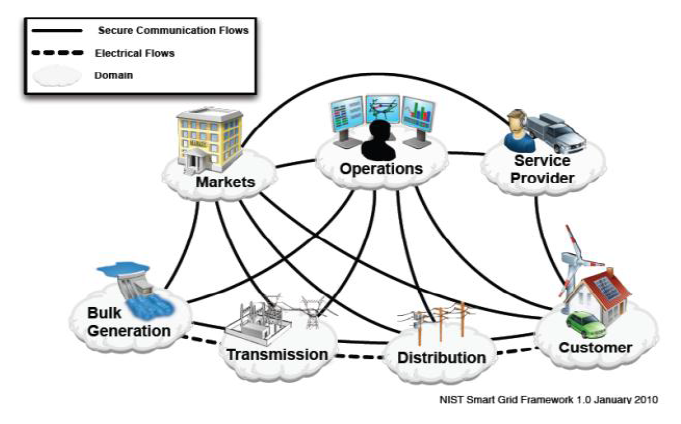
\includegraphics[width=0.95\textwidth]{eikona_000}
\caption[To αφαιρετικό μοντέλο του NIST]{To αφαιρετικό μοντέλο του NIST το οποίο απεικονίζει το Έξυπνο Δίκτυο ως ένα σύνολο οντοτήτων που αλληλεπιδρούν μεταξύ τους\cite{21}}\label{eik00}
\end{figure}

Γενικά οι οντότητες σε κάθε τομέα έχουν κοινούς στόχους και για να τους επιτύχουν πρέπει να συνεργαστούν τόσο μεταξύ τους όσο και με οντότητες άλλων τομέων. Στο σημείο αυτό σημειώνουμε ότι ο διαχωρισμός των οντοτήτων σε τομείς δεν είναι απόλυτος καθότι σε πολλές περιπτώσεις μια οντότητα μπορεί να επιτελεί λειτουργία βασισμένη σε πληροφορία από άλλους τομείς, π.χ. το δίκτυο διανομής αφορά και τον τομέα Διανομής αλλά και τον τομέα Λειτουργιών (αφού εκεί εμπίπτουν τα συστήματα διαχείρισης δικτύων διανομής).
%%%%%%%%%% edw egine merge me to thesen
\section{Προκλήσεις και ανάγκες}

Στην αναφορά \cite{fang} οι προκλήσεις που έχει να αντιμετωπίσει και οι ανάγκες του μελλοντικού έξυπνου δικτύου μεταφοράς συνοψίζονται σε τέσσερις κατηγορίες.
\begin{enumerate}[label=\roman*)]
\item \textbf{Περιβαλλοντικές Προκλήσεις}. Η παραδοσιακή παραγωγή ηλεκτρικής ενέργειας, όντας η μεγαλύτερη δημιουργημένη από τον άνθρωπο πηγή εκπομπής \ce{CO2}, πρέπει να αλλάξει ώστε να αμβλυνθεί η κλιματική αλλαγή. Παράλληλα, έχει προβλεφθεί ανεπάρκεια ορυκτών καυσίμων στις επόμενες δεκαετίες. Φυσικές καταστροφές, όπως θύελλες, σεισμοί και τυφώνες μπορούν εύκολα να καταστρέψουν το δίκτυο μεταφοράς. Τέλος, ο διαθέσιμος και κατάλληλος χώρος για τη μελλοντική επέκταση του δικτύου έχει μειωθεί δραματικά.
\item \textbf{Ανάγκες αγοράς\slash καταναλωτών}. Χρειάζεται να αναπτυχθούν ολοκληρωμένες τεχνολογίες λειτουργίας του συστήματος αλλά και πολιτικές για την αγορά ενέργειας, ώστε να στηρίξουν τη διαφάνεια και την ελευθερία της ανταγωνιστικής αγοράς. Η ικανοποίηση των πελατών από την κατανάλωση ηλεκτρικής ενέργειας θα πρέπει να βελτιωθεί με την παροχή υψηλού λόγου ποιότητας\slash τιμής και με τη δυνατότητα των καταναλωτών να αλληλεπιδρούν με το δίκτυο.
\item \textbf{Προκλήσεις Υποδομής}. Η υπάρχουσα υποδομή μεταφοράς ηλεκτρικής ενέργειας περιέχει στοιχεία που γερνούν γρήγορα. Με την πίεση των αυξανόμενων απαιτήσεων φορτίου, η συμφόρηση του δικτύου γίνεται όλο και χειρότερη. Τα γρήγορα εργαλεία online ανάλυσης, η ευρείας ζώνης παρακολούθηση, οι μετρήσεις και ο έλεγχος, και η γρήγορη και ακριβής προστασία κρίνονται ως απαραίτητα στοιχεία για να βελτιωθεί η αξιοπιστία των δικτύων.
\item \textbf{Καινοτόμες Τεχνολογίες}. Από τη μία πλευρά, οι καινοτόμες τεχνολογίες, συμπεριλαμβανομένων νέων υλικών, προηγμένων ηλεκτρονικών ισχύος και τεχνολογιών επικοινωνιών, δεν είναι ακόμα ώριμες ή εμπορικά διαθέσιμες για την επανάσταση των δικτύων μεταφοράς. Από την άλλη, στο υπάρχον δίκτυο υπάρχει έλλειψη συμβατότητας για να δεχθεί την εφαρμογή spear-point τεχνολογιών στα πρακτικά δίκτυα.
\end{enumerate}
\clearpage
\begin{figure}[tp]
\centering
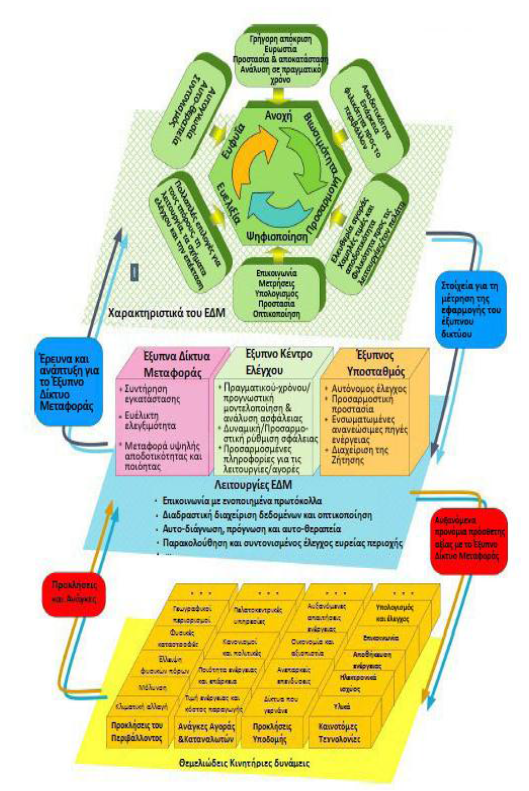
\includegraphics[width=0.95\textwidth]{eikona_02}
\caption[Όραμα ενός έξυπνου δικτύου μεταφοράς]{Όραμα ενός έξυπνου δικτύου μεταφοράς\cite{zwtou}}
\end{figure}
\clearpage

\section{Πλαίσιο και χαρακτηριστικά των έξυπνων δικτύων μεταφοράς}

Στο σχ.~\ref{eik3} παρουσιάζονται τα βασικά χαρακτηριστικά που καλείται να έχει ένα έξυπνο δίκτυο, τα οποία αναλύονται παρακάτω. Όπως φαίνεται, διασυνδέονται με μια στενή σχέση αιτίου-αποτελέσματος το ένα με το άλλο και αποτελούν προκλήσεις που θα πρέπει να ληφθούν σοβαρά υπ'όψη κατά το σχεδιασμό ενός έξυπνου δικτύου.
\begin{figure}[!h]
\centering
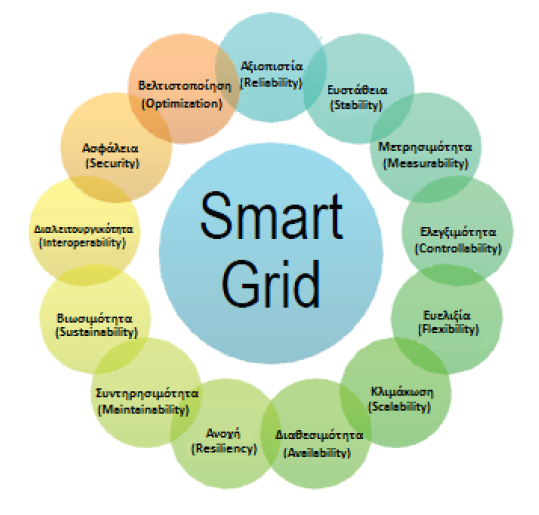
\includegraphics[width=0.76\textwidth]{eikona_03}
\caption[Τα χαρακτηριστικά και οι απαιτήσεις ενός Έξυπνου Δικτύου]{Τα χαρακτηριστικά και οι απαιτήσεις ενός Έξυπνου Δικτύου\cite{zwtou}}\label{eik3}
\end{figure}

\subsection*{Αξιοπιστία και Ευστάθεια (\textenglish{Reliability and Stability})}

Με τον όρο αξιοπιστία αναφερόμαστε στην ικανότητα ενός συστήματος ή και στοιχείων αυτού να εκτελούν τις απαιτούμενες λειτουργίες υπό δεδομένες συνθήκες για καθορισμένο χρονικό διάστημα. Η αξιοπιστία έχει ένα χαρακτηριστικό ανθεκτικότητας. Σε γενικές γραμμές, ερμηνεύει τη λειτουργική υγεία και το βαθμό μεταβλητότητας όλου του συστήματος. Επιπλέον, παρουσιάζει την κατάσταση υψηλής συνοχής, επαναληψιμότητας και φερεγγυότητας που το έξυπνο δίκτυο θα διατηρήσει σύμφωνα με αποτελεσματικές μετρήσεις και εκτιμήσεις. Με την αξιοπιστία απαιτούμε οι βλάβες του συστήματος να συμβαίνουν με μικρή πιθανότητα, ενώ σε περίπτωση που κάτι πάει στραβά, η επίπτωσή του στο συνολικό σύστημα να είναι ελάχιστη και το δυσλειτουργικό στοιχείο να αντικατασταθεί ή να επιδιορθωθεί όσο το δυνατόν συντομότερα. Η αξιοπιστία εξαρτάται από την επίτευξη άλλων καθοριστικών παραγόντων, που περιγράφονται στις παρακάτω υποενότητες.

Η ευστάθεια ενός συστήματος καθορίζει το επίπεδο αξιοπιστίας που το χαρακτηρίζει. Το έξυπνο δίκτυο πρέπει να εγγυάται σταθερότητα της τάσης και του ρεύματος, να περιορίζει τη ζήτηση αιχμής και τη μεταβλητότητα του φορτίου, με την εφαρμογή κατανεμημένης ηλεκτροπαραγωγής (Distributed Generation - DG) και αποθήκευση ενέργειας σε μεγάλες εκτάσεις, και να αποκλείει διάφορα ανεπιθύμητα περιστατικά.

\subsection*{Μετρησιμότητα και Ελεγξιμότητα (\textenglish{Measurability and Controllability})}

Η διακοπή υπηρεσιών και οι βλάβες είναι περιστατικά σοβαρά και υπάρχει μεγάλη πιθανότητα να συμβούν. Είναι σημαντικό να είναι μετρήσιμα και ελέγξιμα με τρόπο ώστε να μπορούν να πραγματοποιηθούν σκόπιμες εκτιμήσεις και αξιολογήσεις. Το έξυπνο δίκτυο είναι σε θέση να εντοπίζει και να διορθώνει λειτουργικές διαταραχές μέσω δυναμικών μετρήσεων και παρακολούθηση πραγματικού χρόνου. Παράλληλα, θα πρέπει να υπάρχει κάποιος βαθμός παρατηρησιμότητας και διαφάνειας με στόχο την αποτελεσματική ανάλυση, διαχείριση, καθώς και την πρόβλεψη και αντίδραση στις μεταβαλλόμενες καταστάσεις του δικτύου. Ο πλούτος πληροφοριών των δεδομένων, που ουσιαστικά καθιστά το δίκτυο έξυπνο πρέπει επίσης να είναι μετρήσιμος, παρατηρήσιμος και διαχειρίσιμος.

\subsection*{Ευελιξία και Κλιμάκωση (\textenglish{Flexibility and Scalability})}

Το δίκτυο κινείται από μια κεντρική δομή σε πολλαπλά αποκεντρωμένα μικροδίκτυα (Microgrids - MGs). Η κλιμάκωση του έξυπνου δικτύου είναι σημαντικό να οριστεί καλά. Μέσω της νησιδοποίησης (islanding), τα μικροδίκτυα προσπαθούν να ενσωματώσουν την κατανεμημένη παραγωγή (DG) και την αποθήκευση ενέργειας για να συνεισφέρουν ενέργεια στις επιχειρήσεις κοινής ωφέλειας σε περιόδους ζήτησης αιχμής. Η λειτουργία της νησίδας εισάγει μια έννοια ενός γιγάντιου έξυπνου δικτύου που αποτελείται από πολλαπλά μικρά έξυπνα δίκτυα. Κάθε τοπικό δίκτυο μπορεί να λειτουργεί αυτόνομα ως προς τη Διαχείριση της Ζήτησης (Demand Side Management - DSM), το μοντέλο ποιότητας και αξιοπιστίας, τη διαχείριση προβλημάτων και τη διαχείριση ασφάλειας.

Η ευελιξία επιτρέπει στο έξυπνο δίκτυο να παρέχει πολλαπλές εναλλακτικές διαδρομές για τη ροή της ενέργειας και των δεδομένων, ενώ επίσης παρέχει επιλογές για να είναι εφικτός ο έλεγχος και η λειτουργία όποτε χρειάζεται. Θα λέγαμε ότι παρουσιάζει τέσσερις πτυχές: \mbox{α) επεκτασιμότητα} για μελλοντική ανάπτυξη με τη διείσδυση καινοτόμων και διαφορετικών τεχνολογιών παραγωγής, β) προσαρμοστικότητα στις ποικίλες γεωγραφικές τοποθεσίες και τα κλίματα, γ) πολλαπλές στρατηγικές ελέγχου για το συντονισμό των αποκεντρωμένων συστημάτων ελέγχου ανάμεσα στους υποσταθμούς και τα κέντρα ελέγχου, \mbox{δ) απρόσκοπτη} συμβατότητα με τα διάφορα στυλ λειτουργίας της αγοράς και plug-and-play ικανότητα να φιλοξενήσει σταδιακή αναβάθμιση, με συστατικά υλικού και λογισμικού, της τεχνολογίας.

Η ευελιξία μπορεί ακόμη να εφαρμοστεί σε ένα σύνολο προτύπων (standards) που λειτουργούν στο δίκτυο, συμπεριλαμβανομένων των ANSI, IEC, PLC, wireless M-Bus και ZigBee, ούτως ώστε να είναι διαθέσιμα και αναβαθμίσιμα σε όλο τον κόσμο.

\subsection*{Διαθεσιμότητα (Availability)}

Η διαθεσιμότητα της ενέργειας και των επικοινωνιών είναι ουσιώδης για τη ζήτηση ενέργειας και πληροφοριών από τους καταναλωτές και βασίζεται στη διαθεσιμότητα των δεδομένων που ανταλλάσσονται στο δίκτυο. Ο βαθμός διαθεσιμότητας πόρων που απαιτείται, ειδικά όταν πρόκειται για θέματα που σχετίζονται με την καθυστέρηση (latency) ή την ασφάλεια, είναι υψηλός. Για παράδειγμα, στα συστήματα προστασίας και ελέγχου της γραμμής η καθυστέρηση χρειάζεται να είναι της τάξης των χιλιοστών του δευτερολέπτου, αλλά μια επίθεση άρνησης υπηρεσίας (Denial of Service - DoS) μπορεί να επιδεινώσει την επίδοση του δικτύου κάνοντας τους servers ή τις υπηρεσίες προσωρινά μη διαθέσιμες. Ο πλεονασμός (redundancy) θα μπορούσε να είναι ένα μέτρο επίλυσης του προβλήματος. Ωστόσο, η αποτελεσματικότητά του θα εξαρτηθεί από το πώς θα σχεδιαστεί το σύστημα για να αποφεύγει παράλληλα το επακόλουθο κόστος της μεγάλης πολυπλοκότητας δικτύου, καθώς και από το θέμα της κλιμάκωσης.

\subsection*{Ανθεκτικότητα (Resiliency)}

O βαθμός της ανθεκτικότητας καθορίζει πόσο πραγματικά αξιόπιστο είναι το έξυπνο δίκτυο όταν συμβαίνουν διάφορα περιστατικά. Γενικά, το δίκτυο θα πρέπει να είναι σε θέση να παρέχει ηλεκτρική ενέργεια στους πελάτες με ασφάλεια και αξιοπιστία παρά τους οποιουσδήποτε εσωτερικούς ή εξωτερικούς κινδύνους. Ειδικά από τη σκοπιά της ασφάλειας, η ανθεκτικότητα αναπαριστά την ικανότητα ανάκτησης και αποκατάστασης μετά από τις οποιεσδήποτε διαταραχές ή δυσλειτουργίες, μέσω μιας εύρωστης διαδικασίας γρήγορης απόκρισης. Η ικανότητα αυτή της αυτό-θεραπείας καθιστά το δίκτυο ικανό να επαναπροσδιορίζεται δυναμικά ώστε να ανακάμψει από επιθέσεις, διακοπές ρεύματος, φυσικές καταστροφές, κακόβουλες δραστηριότητες και βλάβες των κατασκευαστικών στοιχείων του. Τα ευάλωτα ηλεκτρικά στοιχεία είναι πιθανότατα οι γραμμές μεταφοράς και οι σταθμοί, οι μεγάλες μονάδες παραγωγής ενέργειας, καθώς και οι πυρηνικοί σταθμοί με διαρροή. Σχέδια έκτακτης ανάγκης απαιτούνται για την αντιμετώπιση των παραπάνω δυσμενών περιπτώσεων.

\subsection*{Δυνατότητα Συντήρησης (Maintainability)}

Η συντηρησιμότητα αντανακλά ουσιαστικά τη μακροβιότητα και την αξιοπιστία ενός συστήματος. Συνήθως δείχνει την ικανότητά του να εκτελεί αποτελεσματικά και αποδοτικά μια σειρά δράσεων για εργασίες συντήρησης. Οι διαδικασίες που γίνονται ειδικά κατά τη συντήρηση περιλαμβάνουν την επιθεώρηση, την αντιμετώπιση προβλημάτων και την αντικατάσταση. Το έξυπνο δίκτυο θα πρέπει να σχεδιαστεί με τέτοιο τρόπο που να διευκολύνει τη συντήρηση, έτσι ώστε τα διάφορα στοιχεία ενέργειας και επικοινωνιών (π.χ. εγκαταστάσεις, εξοπλισμός, συστήματα, υποσυστήματα, ασφάλεια του δικτύου και διαχείριση) να επιδιορθώνονται γρήγορα και με τρόπο οικονομικά αποδοτικό. Παρομοίως, η υψηλή αποδοτικότητα εργατοώρας, καθώς και των εργαλείων και του εξοπλισμού αποτελεί σημαντικό παράγοντα για το σύστημα συντήρησης του δικτύου.

\subsection*{Βιωσιμότητα (Sustainability)}

Η άνοδος της ανησυχίας για το περιβάλλον αλλά και οι κίνδυνοι από τη ζήτηση αιχμής καθιστούν κρίσιμη απαίτηση για τη λειτουργία του έξυπνου δικτύου μεταφοράς τη βιωσιμότητα, η οποία παρουσιάζεται ως επάρκεια, αποδοτικότητα και φιλικότητα προς το περιβάλλον. Η αύξηση της ζήτησης για ηλεκτρική ενέργεια θα πρέπει να ικανοποιηθεί με την εφαρμογή προσιτών εναλλακτικών ενεργειακών πόρων, την αύξηση εξοικονόμησης ενέργειας μέσω της τεχνολογίας στη λειτουργία του συστήματος παροχής και μετριασμό της συμφόρησης δικτύου. Οι καινοτόμες τεχνολογίες που θα χρησιμοποιηθούν θα πρέπει να προκαλούν λιγότερη μόλυνση ή εκπομπές και να είναι απεξαρτημένες από τον άνθρακα, λαμβάνοντας υπόψη τις περιβαλλοντικές και κλιματικές αλλαγές.

\subsection*{Διαλειτουργικότητα (Interoperability)}

Η αποδοτικότητα και αποτελεσματικότητα της συνολικής επίδοσης του συστήματος θα εξαρτηθεί κατά κύριο λόγο από τη διαλειτουργικότητα που παρουσιάζει η υποδομή. Τα κατασκευαστικά στοιχεία του έξυπνου δικτύου προϋποθέτουν την ύπαρξη ενός συνόλου κοινών και διαλειτουργικών προτύπων για τη διασύνδεση τόσο της ενέργειας όσο και των επικοινωνιών. Αυτή η δυνατότητα απαιτείται κατά την ενσωμάτωση και σύγκλιση διαφόρων τεχνολογιών και πρωτοκόλλων επικοινωνιών, προκειμένου να γίνονται κατανοητά το ένα στο άλλο και να παρέχουν αδιάλειπτη μεταφορά ενέργειας και δεδομένων. Αδέξια αλληλεπίδραση και ενοποίηση μεταξύ των ποικιλόμορφων μερών θα επιβράδυνε το χρόνο απόκρισης και θα υποβάθμιζε τη λειτουργία του συνολικού συστήματος καθώς και την αποδοτικότητα.

\subsection*{Ασφάλεια (Security)}

Η έννοια της ασφάλειας απευθύνεται στις δυσλειτουργίες του συστήματος που οφείλονται σε ανθρώπινα αίτια, όπως εσκεμμένες επιθέσεις και μη εξουσιοδοτημένες τροποποιήσεις. Μια ασφαλής και σίγουρη συνδεσιμότητα μεταξύ προμηθευτών και καταναλωτών παρέχει προστασία για τις κρίσιμες εφαρμογές και τα δεδομένα αλλά και άμυνες ενάντια σε παραβιάσεις της ασφάλειας. Διάφορα υπάρχοντα μέτρα και εργαλεία ασφαλείας αποτελούν στοιχειώδεις απαιτήσεις για το έξυπνο δίκτυο, όπως τα συστήματα Firewall, τα συστήματα ανίχνευσης και αποτροπής εισβολών (IDS/IPS), τα εικονικά ιδιωτικά δίκτυα (virtual private network - VPN), τα εικονικά τοπικά δίκτυα (virtual local area network-VLAN) και ο έλεγχος πρόσβασης.

\subsection*{Βελτιστοποίση (Optimization)}

Η βελτιστοποίηση της λειτουργίας και των στοιχείων ενεργητικού του έξυπνου δικτύου είναι επιτακτική ανάγκη. Μπορεί να επιτευχθεί με τη βοήθεια των προηγμένων τεχνολογιών και των έξυπνων ηλεκτρικών συσκευών (Intelligent electronic devices - IEDs), καθώς και με ευφυή διαχείριση και αυτοματισμό, εξισορροπώντας ταυτόχρονα μια ποικιλομορφία μεταβλητών και tradeoffs. Το έξυπνο δίκτυο καλείται να βελτιστοποιηθεί σύμφωνα με όρους α) αξιοπιστίας της παροχής ηλεκτρικής ενέργειας, β) αποδοτικότητας μετατροπής και χρήσης της ενέργειας, γ)~ποιότητας παραγωγής και διανομής ενέργειας, δ) διαθεσιμότητας για τη μεταφορά ενέργειας και δεδομένων, ε) αποτελεσματικότητας και ακρίβειας των δεδομένων και των επικοινωνιών, στ) χρονικής απόκρισης και διαχείρισης σφαλμάτων, ζ) οικονομικό κέρδος. Εν τω μεταξύ, η μείωση του κόστους κεφαλαίου, η πολυπλοκότητα του δικτύου και η χρήση των πόρων είναι αποφασιστικής σημασίας για το έξυπνο δίκτυο που θα αναπτυχθεί στην πράξη.

Εκτός από όσα απεικονίζονται και αναλύθηκαν παραπάνω, ως επιπλέον ιδιότητες ενός μελλοντικού έξυπνου δικτύου θα μπορούσαμε να σημειώσουμε και τα εξής:

\subsection*{Ψηφιοποίηση (Digitalization)}

Το έξυπνο δίκτυο θα χρησιμοποιεί μια μοναδική, ψηφιακή πλατφόρμα για γρήγορη και αξιόπιστη ανίχνευση, μέτρηση, επικοινωνία, υπολογισμό, έλεγχο, προστασία, απεικόνιση και συντήρηση ολόκληρου του συστήματος μεταφοράς. Πρόκειται για θεμελιώδες χαρακτηριστικό που θα διευκολύνει την υλοποίηση άλλων έξυπνων λειτουργιών. Αυτή η πλατφόρμα χαρακτηρίζεται από φιλική προς το χρήστη απεικόνιση για ενημέρωση ευαίσθητων καταστάσεων αλλά και από υψηλή ανοχή προς ανθρωπογενή λάθη.

\subsection*{Ευφυΐα (Intelligence)}

Ευφυείς τεχνολογίες και ανθρώπινη τεχνογνωσία θα ενσωματωθούν στο έξυπνο δίκτυο μεταφοράς. Αυτό-επίγνωση της κατάστασης λειτουργίας του συστήματος θα είναι διαθέσιμη με τη βοήθεια online ανάλυσης στο πεδίο του χρόνου, όπως ανάλυση της σταθερότητας τάσης\slash γωνίας και της ασφάλειας. Θα υπάρχει, επίσης, αυτό-θεραπεία για να ενισχύσει την ασφάλεια του δικτύου μεταφοράς μέσω συντονισμένων σχημάτων προστασίας και ελέγχου.

\subsection*{Προσαρμογή (Customization)}

Ο σχεδιασμός του έξυπνου δικτύου μεταφοράς θα είναι, για την ευκολία των φορέων εκμετάλλευσης, προσαρμοσμένος στον πελάτη, χωρίς να χάνει τις λειτουργίες του και τη διαλειτουργικότητά του. Επίσης, θα εξυπηρετεί τους πελάτες παρέχοντας περισσότερες επιλογές κατανάλωσης ενέργειας για έναν υψηλότερο λόγο ποιότητας\slash τιμής. Το έξυπνο δίκτυο θα απελευθερώσει περαιτέρω την αγορά ενέργειας με την αύξηση της διαφάνειας και τη βελτίωση του ανταγωνισμού για τους συμμετέχοντες στην αγορά.

\section{Προκλήσεις αξιοπιστίας του δικτύου}

Η αξιοπιστία βρίσκεται στην πρώτη γραμμή του σχεδιασμού και της λειτουργίας του δικτύου λόγω του ιδιαίτερα υψηλού κόστους των απρογραμμάτιστων διακοπών παροχής ηλεκτρικής ενέργειας. Τα σύγχρονα δίκτυα βρίσκονται αντιμέτωπα με πολλούς παράγοντες που επηρεάζουν την αξιοπιστία και γι’ αυτό γίνεται πιο δύσκολο να επιτύχουν τους στόχους για ενίσχυσή της. Έτσι επιτακτική είναι η ανάγκη για αντιμετώπιση των παρακάτω προκλήσεων που δυσχεραίνουν την αξιοπιστία του δικτύου. Για την αντιμετώπιση των προκλήσεων αυτών αναπόφευκτη είναι η ώθηση προς ένα πιο έξυπνο δίκτυο ικανό να μετριάσει τα προβλήματα του σύγχρονου δικτύου. Οι προκλήσεις που ταυτόχρονα αποτελούν κινητήριες δυνάμεις για την ανάπτυξη των έξυπνων δικτύων είναι \cite{39}:
\begin{itemize}
\item[-] Η επιδείνωση της συμφόρησης του δικτύου διανομής, εξαιτίας μεταξύ άλλων της αβεβαιότητας, της ποικιλομορφίας και της αυξημένης ενέργειας που παράγεται από ανανεώσιμες πηγές συνδεδεμένες σ’ αυτό
\item[-] Οι πολυάριθμες και μεγαλύτερου μεγέθους μεταφορές σε πιο μακρινές αποστάσεις που αυξάνουν την αστάθεια και μειώνουν τα περιθώρια αξιόπιστης λειτουργίας
\item[-]Το δίκτυο που λειτουργεί στα όρια του συχνά λόγω:
\begin{itemize}
\item[$\bullet$] Ανεπαρκών επενδύσεων
\item[$\bullet$] Της αυξανόμενης κατανάλωσης ενέργειας και της υψηλότερης μέγιστης ζήτησης ισχύος
\item[$\bullet$] Της γήρανσης της υποδομής
\item[$\bullet$] Της μεγιστοποίησης της χρησιμοποίησης του εξοπλισμού με χρήση σύγχρονων εργαλείων για παρακολούθηση, ανάλυση και έλεγχο
\end{itemize}
\item[-] Η ενοποίηση των φορέων λειτουργίας που δημιουργεί πιο σύνθετα προβλήματα περιορίζοντας τους χρόνους αποφάσεων και τα περιθώρια λάθους
\item[-] Η μαζική διείσδυση της διανεμημένης παραγωγής που καθιστά ασαφή την διάκριση μεταξύ μεταφοράς και διανομής και επιτείνει την πολυπλοκότητα και την αστάθεια του δικτύου
\end{itemize}

\section{Οι επιδράσεις των κυριότερων στοιχείων του έξυπνου δικτύου στην αξιοπιστία}

\subsection{Ανανεώσιμες πηγές}

Οι ταχύτερα αναπτυσσόμενες μορφές ανανεώσιμων πηγών ενέργειας είναι η αιολική και η ηλιακή. Εγγενές πρόβλημα της αιολικής ενέργειας είναι η περιορισμένη προβλεψιμότητά της που υποδεικνύεται από τους χαμηλούς συντελεστές χρησιμοποίησης (20\%-40\%) σε σύγκριση με αυτούς των συμβατικών γεννητριών \cite{40}. Αυτό δημιουργεί προβλήματα στον έλεγχο και την αξιοπιστία του δικτύου \cite{41}. Η μεταβλητότητα της αιολικής ενέργειας δεν συμπίπτει απαραίτητα με την μεταβλητότητα του φορτίου και γι’ αυτό δεν συνεισφέρει πάντα στην κάλυψη της μέγιστης ζήτησης, αφού υπάρχει πιθανότητα στις ώρες αιχμής να μην είναι διαθέσιμη.

Η άφθονη ηλιακή ενέργεια που φτάνει στην επιφάνεια της γης ξεπερνά κατά περίπου 1000 φορές την ενέργεια που παράγεται από τη σημερινή παγκόσμια κατανάλωση ορυκτών καυσίμων κάθε χρόνο \cite{42}. Μέχρι το 2020 η παραγωγή ισχύος από την εκμετάλλευση της ηλιακής ενέργειας αναμένεται να φτάσει τα 16GW \cite{43}.Οι δύο επικρατούσες τεχνολογίες εκμετάλλευσης της ενέργειας αυτής είναι τα φωτοβολταϊκά και τα ηλιοθερμικά συστήματα. Η μεταβλητότητα της ηλιακής ενέργειας εξαρτάται σε μεγάλο βαθμό από το κλίμα και την διαθεσιμότητα ηλιακής ακτινοβολίας. Οι συντελεστές χρησιμοποίησης των φωτοβολταϊκών είναι μεταξύ 10-20\%, ενώ για τα θερμικά ηλιακά συστήματα με δυνατότητα αποθήκευσης μπορεί να φτάσει έως 70\% \cite{44}. Οι μεγάλης κλίμακας ηλιακές πηγές μπορεί να βρίσκονται μακριά από τα φορτία και κατά συνέπεια να αντιμετωπίζουν διάφορους περιορισμούς μεταφοράς. Ωστόσο, η ηλιακή ενέργεια συμπίπτει με την αυξημένη ζήτηση κατά τους θερινούς μήνες οπότε η αυξημένη διαθεσιμότητά της εκείνες τις περιόδους μπορεί να καλύψει τα αυξημένα φορτία των κλιματιστικών.

Από την προσέγγιση της αξιοπιστίας, οι ανανεώσιμες πηγές ενέργειας όπως η γεωθερμία και η βιομάζα συμπεριφέρονται παρόμοια με την συμβατική παραγωγή ενέργειας. Σε αντίθεση με την αιολική και την ηλιακή ενέργεια που γενικά έχουν δυσμενή επίδραση στην αξιοπιστία του δικτύου εξαιτίας:
\begin{itemize}
\item Της μεταβλητότητας και των χαμηλών συντελεστών χρησιμοποίησης
\item Της χαμηλής συσχέτισής τους με τις καμπύλες φορτίου ειδικά για την αιολική ενέργεια
\item Της μεγάλης δυσκολίας πρόβλεψης για μακροχρόνιο διάστημα
\item Της συμφόρησης στη μεταφορά και τη διανομή εξαιτίας της εγκατάστασης μεγάλων και διανεμημένων μονάδων
\item Των ζητημάτων λειτουργικής απόδοσης όπως ο συγχρονισμός και η ρύθμιση τάσης
\end{itemize}

Οι συμβατικοί τρόποι παραγωγής ηλεκτρικής ενέργειας (υδροηλεκτρικοί σταθμοί, ατμοηλεκτρικοί σταθμοί κτλ.) έχουν χρησιμοποιηθεί ως λύση στην κάλυψη της μεταβλητής ζήτησης των καταναλωτών. Όμως η ραγδαία ανάπτυξη των ανανεώσιμων πηγών ενέργειας κάνει επιτακτική την ανάγκη απόκρισης της ζήτησης και εγκατάστασης συστημάτων αποθήκευσης, που μπορούν να συμπληρώσουν τις συμβατικές λύσεις \cite{39}.

\subsection{Διαχείρηση φορτίου - Απόκριση ζήτησης}

Η διαχείριση του φορτίου περιλαμβάνει την μείωση του φορτίου ως απόκριση σε κρίσιμες καταστάσεις και\slash ή σε υψηλές τιμές της ηλεκτρικής ενέργειας. Τέτοιες συνθήκες επικρατούν κυρίως κατά την διάρκεια περιόδων αιχμής ή σε περιπτώσεις κορεσμένης λειτουργίας του δικτύου. Η μείωση του φορτίου ως πρωτοβουλία του καταναλωτή αναφέρεται ως απόκριση της ζήτησης. Η απόκριση της ζήτησης σε καταστάσεις μη έκτακτης ανάγκης εκτιμάται σε εύρος 5\% με 10\% του μέγιστου φορτίου και μπορεί να προσφέρει σημαντικά οφέλη, περιορίζοντας τις ανάγκες για επιπλέον παραγωγή ηλεκτρικής ενέργειας και μειώνοντας τις τιμές του ηλεκτρισμού \cite{45}. Η απόκριση ζήτησης δεν μεταβάλλει σε αξιοσημείωτο βαθμό την συνολική κατανάλωση ενέργειας, αφού μεγάλο τμήμα της ενέργειας που εξοικονομείται κατά την περικοπή του φορτίου καταναλώνεται σε κάποια άλλη χρονική στιγμή. Ως αποτέλεσμα αυτού του χαρακτηριστικού της απόκρισης ζήτησης προκύπτει μια πιο επίπεδη καμπύλη φορτίου.

Η απόρριψη φορτίου (Load Shedding) για προστασία του δικτύου σε επείγουσες καταστάσεις εφαρμόζεται είτε με εντολή από τον διαχειριστή του συστήματος είτε μέσω ρελέ προστασίας σε περιπτώσεις υπότασης ή\slash και μειωμένης συχνότητας. Το έξυπνο δίκτυο μπορεί να ενισχύσει τη διαχείριση του φορτίου ώστε να εκτελείται με περισσότερη ευφυΐα και μεγαλύτερη συμμετοχή από τους καταναλωτές. Η διαφορετική χρέωση της ηλεκτρικής ενέργειας ανάλογα με την χρονική περίοδο, σε ένα έξυπνο δίκτυο, καθιστά δυνατή την αυξημένη εκούσια συμμετοχή των καταναλωτών μέσω αυτοματοποιημένης ή χειρονακτικής απόκρισης και μέσω επικοινωνίας του καταναλωτή με την εταιρία παροχής ή τον διαχειριστή του συστήματος. Η απόκριση της ζήτησης, με την ικανότητά της να συνεισφέρει στη διαμόρφωση μιας πιο επίπεδης καμπύλης φορτίου, μπορεί να χρησιμοποιηθεί και για την παροχή βοηθητικών υπηρεσιών με αποτέλεσμα την βελτίωση της αξιοπιστίας του δικτύου \cite{39}.

\subsection{Συσκευές αποθήκευσης}

Ο κύριος τρόπος αποθήκευσης είναι τα συστήματα άντλησης και αποθήκευσης υδραυλικής ενέργειας \cite{39}. Ωστόσο, η δυνατότητα περαιτέρω ανάπτυξης αυτών των συστημάτων είναι περιορισμένη σε σχέση με την ανάγκη για αποθήκευση ενέργειας που έχει προκύψει, εξαιτίας της μεταβλητότητας της συμπεριφοράς των αναπτυσσόμενων ανανεώσιμων πηγών, της αιολικής και της ηλιακής ενέργειας. Διάφορες τεχνολογίες αποθήκευσης αναδύονται για να συμπληρώσουν το κενό. Η μπαταρία φαίνεται να είναι η πιο υποσχόμενη από αυτές λόγω των πρόσφατων βελτιώσεων στην τεχνολογία της και στην οικονομία χώρου που προσφέρει. Η αποθήκευση γρήγορης απόκρισης, που ουσιαστικά δρα ως <<ανακυκλωτής>> ενέργειας, έχει την τάση να επιδρά στην καμπύλη ζήτησης μετασχηματίζοντάς την σε πιο επίπεδη και ως αναμενόμενο αποτέλεσμα αυτού ενισχύει την αξιοπιστία του δικτύου. Οι μπαταρίες μπορούν να καταστήσουν δυνατή την πραγματοποίηση ταχύτατων ελέγχων σε έξυπνα δίκτυα, καθώς έχουν τη δυνατότητα να αποκρίνονται μέσα σε κλάσματα του δευτερολέπτου. Με διαφορετικού μεγέθους αποθήκευση διανεμημένη κατά μήκος του δικτύου, σε τελικούς καταναλωτές, σε υποσταθμούς αλλά και σε μεγάλους σταθμούς παραγωγής, μπορεί να επιτευχθεί αποσυμφόρηση των δικτύων διανομής και μεταφοράς \cite{39}.

\subsection{Ηλεκτροκίνητα μέσα μεταφοράς}

Τα ηλεκτρικά οχήματα (PEV, eCAR) συνεχίζουν να γίνονται όλο και πιο δημοφιλή όσο οι περιβαλλοντικές ανησυχίες εντείνονται. Αποτελούν ένα σπουδαίο μέσο για να περιοριστεί η εξάρτηση από τα ορυκτά καύσιμα και η εκπομπή αερίων του θερμοκηπίου στην ατμόσφαιρα. Αναμένεται να αποτελέσουν σημαντικό παράγοντα της μελλοντικής αύξησης του φορτίου. Από την πλευρά της αξιοπιστίας, τα ηλεκτρικά οχήματα διακρίνονται από χαρακτηριστικά παρόμοια με αυτά της απόκρισης ζήτησης και της αποθήκευσης ηλεκτρικής ενέργειας \cite{39}. Όμως, δεδομένου ότι θα επιφέρουν ραγδαία αύξηση του φορτίου, τα PEVs μπορούν να επιβαρύνουν την μεταβλητότητα της ζήτησης και τα σχετικά με την αξιοπιστία προβλήματα ανάλογα με τα συστήματα φόρτισης και τις συνήθειες του καταναλωτή. Μεγάλης διάρκειας επαναφόρτιση οδηγεί σε μη διαθεσιμότητα του οχήματος κατά το χρονικό διάστημα αυτό. Κάτι τέτοιο ενδέχεται να μην γίνει αποδεκτό από τον καταναλωτή. Από την άλλη πλευρά, η σύντομη επαναφόρτιση είναι πιθανό να αυξήσει την συμφόρηση στο δίκτυο διανομής \cite{39}.

\section{Η παρούσα εργασία στα Έξυπνα Δίκτυα Ενέργειας}

Σύμφωνα με το μοντέλο που παρουσιάστηκε στην ενότητα~\ref{dipl}, το αντικείμενο της συγκεκριμένης Διπλωματικής Εργασίας εντάσσεται στον τομέα των Πελατών. Οι συσκευές μέτρησης, το expansion board καθώς και το λογισμικό που <<τρέχει>> το BeagleBone που τις ελέγχει, έχουν σχεδιαστεί και υλοποιηθεί από την εταιρεία Meazon Α.Ε.~. Με την προσθήκη του expansion board στο BeagleBone, καταφέραμε να έχουμε συνδεσιμότητα στο Διαδίκτυο μέσω του δικτύου κινητής τηλεφωνίας, έτσι ώστε να μπορούμε να εγκαταστήσουμε μετρητικές συσκευές, τις οποίες θα ελέγχουμε απομακρυσμένα και θα βλέπουμε τα μετρητικά τους δεδομένα,  σε μέρη όπου δεν υπάρχει η δυνατότητα ενσύρματης σύνδεσης στο Διαδίκτυο μέσω του τηλεφωνικού δικτύου, ή απλά σε περιπτώσεις που κρίνεται πιο οικονομικά συμφέρουσα η λύση ενός πλάνου για παροχή Internet από πάροχο κινητής τηλεφωνίας σε σχέση με το κόστος μιας σύνδεσης σταθερού τηλεφώνου.

\chapter[Επικοινωνία μεταξύ συσκευών - Μ2Μ]{Επικοινωνία μεταξύ συσκευών (Machine to Machine Communication - M2M)}

Η Μ2Μ επικοινωνία χρησιμοποιεί τεχνολογίες για να επιτρέψει τόσο σε ασύρματα όσο και σε ενσύρματα συστήματα να συνδεθούν με συσκευές της ίδιας ικανότητας. Επιτρέπει σε συσκευές, όπως υπολογιστές, αισθητήρες, ενσωματωμένα συστήματα, κινητά, να επικοινωνούν μεταξύ τους και να παίρνουν αποφάσεις με ελάχιστη ανθρώπινη παρέμβαση. Οι συσκευές, δηλαδή, διαθέτουν πλέον την ευφυΐα να αποφασίζουν αυτόνομα βάσει των δεδομένων που συλλέγουν οι ίδιες ή άλλες συσκευές. Η τεχνολογία αυτή χρησιμοποιεί μια συσκευή (όπως έναν αισθητήρα ή ένα μετρητή) για να καταγράψει ένα γεγονός (όπως η θερμοκρασία, το επίπεδο αποθεμάτων κλπ.) το οποίο αναμεταδίδεται μέσω ενός δικτύου (ασύρματο, ενσύρματο ή υβριδικό) σε μια εφαρμογή (πρόγραμμα λογισμικού), η οποία μεταφράζει το καταγεγραμμένο γεγονός σε χρήσιμη πληροφορία (για παράδειγμα, αντικείμενα που χρειάζονται ανεφοδιασμό).

Βασικές εφαρμογές είναι:
\begin{itemize}
\item Σύνδεση μηχανών\slash συσκευών με άλλες μηχανές, π.χ. απομακρυσμένα περιβάλλοντα παραγωγής
\item Σύνδεση μηχανών με τα κέντρα υπηρεσιών, π.χ. αυτοκίνητα που ενημερώνουν τα κέντρα εξυπηρέτησης για θέματα συντήρησης
\item Σύνδεση κέντρων υπηρεσιών με τις μηχανές, π.χ. αυτόματοι πωλητές που αναφέρουν την κατάσταση των αποθεμάτων σε ένα κεντρικό σύστημα καταγραφής
\item Σύνδεση οχημάτων με μηχανές, π.χ. διαχείριση και τοποθεσία στόλου
\end{itemize}
Η επικοινωνία μεταξύ συσκευών είναι μια νέα ιδέα, προερχόμενη από την αρχική τεχνολογία της τηλεμετρίας, που χρησιμοποιείται για αυτόματη μετάδοση και μέτρηση των δεδομένων από απομακρυσμένες πηγές, με ενσύρματο, ασύρματο ή άλλο τρόπο. Η ιδέα της τηλεμετρίας –απομακρυσμένες συσκευές και αισθητήρες που συλλέγουν και στέλνουν δεδομένα σε ένα κεντρικό σημείο για ανάλυση, είτε από ανθρώπους είτε από υπολογιστές– σίγουρα δεν είναι καινούρια. Η Μ2Μ τεχνολογία αναβαθμίζει αυτή την ιδέα εφαρμόζοντας σύγχρονη τεχνολογία δικτύωσης. Χρησιμοποιεί, δηλαδή, παρόμοιες τεχνολογίες αλλά πιο σύγχρονες εκδοχές τους. Η κύρια διαφορά μεταξύ τηλεμετρίας και Μ2Μ έγκειται στις επιχειρηματικές και επιχειρησιακές πτυχές, που θα επιτρέψουν στην Μ2Μ να εξαπλωθεί με πολλούς τρόπους.

Τρεις πολύ διαδεδομένες τεχνολογίες –τα ασύρματα δίκτυα αισθητήρων, το Διαδίκτυο και οι προσωπικοί υπολογιστές– ενώνονται για να δημιουργήσουν την επικοινωνία μεταξύ συσκευών, ή για συντομία Μ2Μ. Η ιδέα υπόσχεται να προωθήσει τη χρήση της τηλεμετρίας από επιχειρήσεις, κυβερνήσεις αλλά και ιδιώτες. Οι Μ2Μ επικοινωνίες, για παράδειγμα, μπορούν να χρησιμοποιηθούν για την πιο αποτελεσματική παρακολούθηση της κατάστασης σημαντικών δημοσίων υποδομών, όπως γεφυρών ή εγκαταστάσεων επεξεργασίας του νερού, με μικρότερη ανθρώπινη παρέμβαση. Μπορεί να βοηθήσει τις επιχειρήσεις να διατηρούν αποθέματα ή να διευκολύνει τους επιστήμονες να διεξάγουν έρευνα. Καθώς στηρίζεται σε κοινή τεχνολογία, θα μπορούσε επίσης να βοηθήσει έναν οικιακό χρήστη ακόμα και σε απλές εργασίες, όπως να διατηρήσει το ιδανικό γκαζόν ή να φτιάξει τη λίστα με τα ψώνια απλά με το πάτημα ενός κουμπιού.

\section{Τηλεμετρία εναντίον M2M επικοινωνιών}

Στην επικοινωνία μεταξύ συσκευών, ένας απομακρυσμένος αισθητήρας συλλέγει δεδομένα και τα στέλνει ασύρματα σε ένα δίκτυο, από όπου κατόπιν δρομολογούνται, συχνά μέσω του Διαδικτύου, σε έναν εξυπηρετητή όπως έναν προσωπικό υπολογιστή. Από αυτό το σημείο, τα δεδομένα αναλύονται και αξιοποιούνται, σύμφωνα με το λογισμικό σε ισχύ.

Η τεχνολογία της τηλεμετρίας, με πολλούς τρόπους, ήταν ο πρόδρομος των πιο προηγμένων Μ2Μ συστημάτων επικοινωνιών. Τόσο η τηλεμετρία όσο και οι επικοινωνίες Μ2Μ μεταδίδουν δεδομένα μέσω ενός αισθητήρα. Η σημαντικότερη διαφορά μεταξύ των δύο είναι ότι αντί για ένα τυχαίο ραδιοσήμα, οι Μ2Μ επικοινωνίες χρησιμοποιούν υπάρχοντα δίκτυα, όπως τα ασύρματα δίκτυα που χρησιμοποιούνται από το κοινό, για να μεταδίδουν τα δεδομένα.

Οι αισθητήρες στις παλαιότερες επικοινωνίες τηλεμετρίας, ωστόσο, ήταν άκρως εξειδικευμένοι και συχνά χρειάζονταν ισχυρές πηγές ενέργειας για τη μετάδοση των δεδομένων. Επίσης, η συλλογή των δεδομένων μπορεί να ήταν ανομοιογενής εάν ένας απομακρυσμένος αισθητήρας βρισκόταν σε <<βνκρό σημείο>> και, ασφαλώς, η ανάλυση των δεδομένων υλοποιούνταν από ό,τι σήμερα θεωρούμε απαρχαιωμένους υπολογιστές.

Οι σύγχρονες Μ2Μ επικοινωνίες αποτελούν τεράστια βελτίωση σε αυτά τα συστήματα. Η πρόοδος της τεχνολογίας αισθητήρων προσφέρει αυξημένη ευαισθησία και ακρίβεια. Επίσης, οι υπολογιστές και το λογισμικό που εκτελούν τις αναλύσεις λειτουργούν σε ταχύτερο ρυθμό. Ωστόσο, η εκρηκτική αύξηση των δημοσίων ασύρματων δικτύων είναι πιθανότατα ο μεγαλύτερος λόγος που οι Μ2Μ επικοινωνίες έχουν επεκταθεί προς πολύ περισσότερους τομείς.

\section{Πώς λειτουργεί η τεχνολογία M2M}

Το να δουλέψει ένα σύστημα επικοινωνίας μεταξύ συσκευών είναι μια βήμα-προς-βήμα διαδικασία. Τα κύρια στοιχεία που εμπλέκονται είναι αισθητήρες, ένα ασύρματο\slash ενσύρματο δίκτυο και ένας υπολογιστής, πιθανώς συνδεδεμένος στο Διαδίκτυο.

Πρώτα από όλα, πρέπει να τοποθετηθούν οι αισθητήρες σε στρατηγικής σημασίας σημεία. Από τους αισθητήρες αποστέλλονται δεδομένα πραγματικού χρόνου στο δίκτυο, που συχνά συνδέεται στο διαδίκτυο και τελικά, είτε μηχανικοί είτε αυτοματοποιημένα συστήματα θα παρακολουθούν την εισερχόμενη αυτή ροή δεδομένων χρησιμοποιώντας υπολογιστές με εξειδικευμένο λογισμικό.
\begin{table}[ht]
\centering
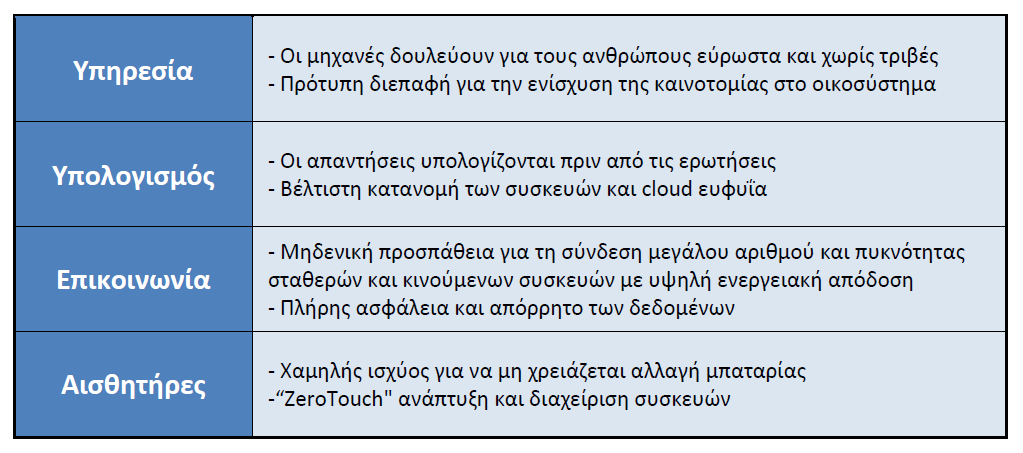
\includegraphics[width=0.95\textwidth]{eikona_04}
\caption[Στοιχεία επικοινωνίας M2M και προκλήσεις]{Κύρια στοιχεία της επικοινωνίας M2M και οι προκλήσεις τους\cite{zwtou}}
\end{table}

Όπως φαίνεται και στον παρακάτω πίνακα, η τεχνολογία Μ2Μ μπορεί να χωριστεί σε τέσσερα κύρια επίπεδα. Οι αισθητήρες συλλέγουν τα δεδομένα, οι μονάδες επικοινωνίας μεταδίδουν τις πληροφορίες που έχουν συγκεντρωθεί, οι υπολογιστικές μονάδες αναλύουν τις πληροφορίες και τα στρώματα υπηρεσιών αναλαμβάνουν δράση.

Ένα Μ2Μ δίκτυο επικοινωνιών αποτελείται από ένα σύνολο Μ2Μ κόμβων και Μ2Μ πυλών. Όπως φαίνεται και στο σχ.~\ref{eik5}(α), ένας Μ2Μ κόμβος διαθέτει πολλαπλούς αισθητήρες για τη συλλογή διαφορετικών τύπων δεδομένων (π.χ. θερμοκρασία, υγρασία) και έναν πομποδέκτη για τη μετάδοση των δεδομένων σε μια Μ2Μ πύλη μέσω επικοινωνιακών πρωτοκόλλων, π.χ. WiFi, ZigBee, UMTS, LTE, WiMAX. Μέσα από ένα σύστημα προσδιορισμού θέσης (π.χ. GPS) ένας κόμβος Μ2Μ μπορεί να λάβει πληροφορίες για τη θέση του. Μια Μ2Μ πύλη, η οποία συνήθως είναι εφοδιασμένη με μόνιμη παροχή ρεύματος, έχει ισχυρή ικανότητα υπολογισμού και μετάδοσης. Βασικό καθήκον της Μ2Μ πύλης είναι να εκτελεί υπολογισμούς επί των συλλεγμένων δεδομένων.
\begin{figure}[!hb]
\centering
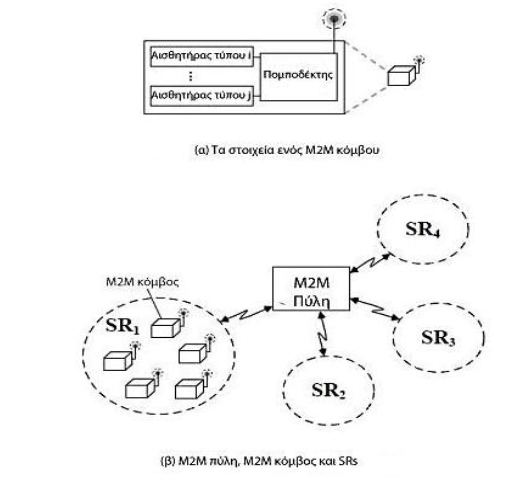
\includegraphics[scale=0.65]{eikona_05}
\caption[Η αρχιτεκτονική του δικτύου ενός συστήματος M2M]{Η αρχιτεκτονική του δικτύου ενός συστήματος M2M\cite{zwtou}}\label{eik5}
\end{figure}
\clearpage

Η πιο πολλά υποσχόμενη Μ2Μ εφαρμογή είναι η πραγματικού χρόνου παρακολούθηση. Σε αυτού του είδους τις εφαρμογές, η περιοχή παρακολούθησης ενός Μ2Μ δικτύου επικοινωνίας διαιρείται σε διάφορες περιοχές ανίχνευσης (Sensing Regions – SRs). Σε κάθε περιοχή μπορεί να υπάρχουν ένας ή περισσότεροι τύποι δεδομένων που πρόκειται να συλλεχθούν και οι τιμές για ένα συγκεκριμένο τύπο από διαφορετικούς Μ2Μ κόμβους είναι πάνω κάτω οι ίδιες σε μια συγκεκριμένη χρονική περίοδο. Το σχ.~\ref{eik5}(β) παρουσιάζει ένα παράδειγμα ενός Μ2Μ δικτύου με τέσσερις SRs. Στο συγκεκριμένο παράδειγμα, υπάρχουν μια Μ2Μ πύλη και πέντε Μ2Μ κόμβοι στην περιοχή SR1.

Κάθε Μ2Μ κόμβος μπορεί να έχει διάφορες ικανότητες ανίχνευσης καθώς κάθε κόμβος μπορεί να διαθέτει διαφορετικού τύπου αισθητήρες ώστε να συλλέγει διαφορετικά είδη δεδομένων. Υπάρχουν δυο καταστάσεις λειτουργίας για έναν Μ2Μ κόμβο: ενεργή λειτουργία (active mode) και λειτουργία αδράνειας (sleep mode). Η περίοδος που ο κόμβος βρίσκεται σε ενεργή κατάσταση (κατάσταση αδράνειας) καλείται ενεργή περίοδος (περίοδος αδράνειας). Κατά την ενεργή περίοδο ο κόμβος συλλέγει τα δεδομένα από τους αισθητήρες του και έπειτα τα μεταδίδει, μαζί με πληροφορίες χρόνου και τοποθεσίας, στην πύλη. Μετά τη μετάδοση ο κόμβος μεταβαίνει σε κατάσταση αδράνειας, στην οποία μένει για κάποιο χρονικό διάστημα, ώστε να ελαχιστοποιεί την κατανάλωση ενέργειας.

Μελλοντικά, ένας τεράστιος αριθμός αισθητήρων πρόκειται να εγκατασταθεί. Το κόστος εξυπηρέτησης τέτοιων αισθητήρων αποτελεί σημαντική ανησυχία. Ως εκ τούτου, αποτελεί πρόκληση μια τεχνολογία αισθητήρων που απαιτεί ελάχιστη ή ακόμα και μηδενική προσπάθεια για την ανάπτυξη και συντήρησή της. Επιπλέον, ένα σημαντικό κόστος της υπηρεσίας αισθητήρων είναι η αντικατάσταση μπαταριών. Είναι συχνά σχεδόν αδύνατο να αντικατασταθούν οι μπαταρίες αισθητήρων από τη στιγμή που αυτοί τοποθετηθούν. Συνεπώς, ακόμα μία πρόκληση είναι ο σχεδιασμός αισθητήρων χαμηλής ισχύος ή σχεδιασμός τέτοιος ώστε να μην απαιτείται αλλαγή μπαταρίας κατά τη διάρκεια ζωής του αισθητήρα.

Αφότου οι αισθητήρες συλλέξουν τα δεδομένα, το επόμενο βήμα είναι να κοινοποιήσουν τις πληροφορίες που συγκέντρωσαν. Πολλοί από τους αισθητήρες θα συνδέονται ασύρματα μέσω συστημάτων όπως Bluetooth, WiFi, ή 3G\slash 4G κυψελωτά δίκτυα. Η σύνδεση του αυξανόμενου αριθμού συσκευών είναι μεγάλη πρόκληση. Οι περισσότεροι σταθμοί βάσης έχουν σχεδιαστεί να παρέχουν ένα ορισμένο επίπεδο ποιότητας υπηρεσίας μέχρι ένα συγκεκριμένο αριθμό χρηστών. Όταν υπάρχουν πάρα πολλοί χρήστες ταυτόχρονα, κάποιοι από αυτούς δε θα λάβουν υπηρεσία. Δεδομένου ότι ο αριθμός των συσκευών θα είναι τάξεις μεγέθους μεγαλύτερος από τον αριθμό των ανθρώπινων χρηστών, το πρόβλημα αυτό θα γίνει ακόμα πιο σοβαρό.

Οι συνδεδεμένες συσκευές (αισθητήρες) μπορούν να παράγουν ωκεανούς δεδομένων. Σύμφωνα με τη Cisco, ο αριθμός των αντικειμένων στο διαδίκτυο υπερέβη τον αριθμό των ανθρώπων το 2008 ή το 2009, μια τάση που επιταχύνει κάθε χρόνο. Έτσι, στο μέλλον η ποσότητα των δεδομένων που παράγονται από συσκευές θα είναι κατά πολύ μεγαλύτερη από αυτή που παράγεται από τους ανθρώπους. Ωστόσο, χρειαζόμαστε επίπεδα ευφυΐας για να μετατρέψουμε αυτά τα δεδομένα σε σοφία (Σχ.~\ref{eik6}). Σε αυτή τη νέα εποχή πληροφορικής, η ανάλυση των δεδομένων και το πλαίσιό της θα διαδραματίσουν ένα σημαντικό ρόλο.

Τελικά, μετά την κατανόηση των πλαισίων, οι μηχανές είτε θα πρέπει να λάβουν κατάλληλη δράση, είτε να παρακινήσουν τους ανθρώπους για κατάλληλη δράση. Ιδανικά, θα πρέπει οι συσκευές να δουλεύουν για τους ανθρώπους.
\begin{figure}[hb]
\centering
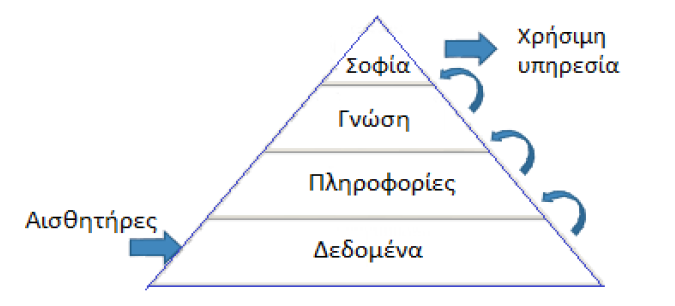
\includegraphics[width=0.9\textwidth]{eikona_06}
\caption[Πυραμίδα της γνώσης]{Διαδικασία μετατροπής των ακατέργαστων πρώτων δεδομένων σε πληροφορίες, γνώση και τελικά χρήσιμη υπηρεσία. (Πυραμίδα της γνώσης)\cite{pyramid}}\label{eik6}
\end{figure}
\clearpage

\section{Εφαρμογές των επικοινωνιών M2M}

Είναι εύκολο να καταλάβει κανείς γιατί οι επικοινωνίες μηχανής-με-μηχανή έχουν τόσες πολλές εφαρμογές. Με καλύτερους αισθητήρες, ασύρματα δίκτυα και αυξημένη υπολογιστική ικανότητα, η ανάπτυξη μιας Μ2Μ επικοινωνίας έχει νόημα για πολλούς τομείς.

Οι \textbf{επιχειρήσεις κοινής ωφελείας}, για παράδειγμα, χρησιμοποιούν Μ2Μ επικοινωνίες τόσο στη συλλογή ενεργειακών προϊόντων, όπως το πετρέλαιο και το φυσικό αέριο, όσο και στην τιμολόγηση των πελατών. Ο \textbf{έλεγχος της κυκλοφορίας} είναι ακόμα ένα δυναμικό περιβάλλον που μπορεί να επωφεληθεί από τις επικοινωνίες Μ2Μ. Σε ένα τυπικό σύστημα, αισθητήρες παρακολουθούν μεταβλητές όπως είναι η ένταση της κίνησης και η ταχύτητα και στέλνουν αυτές τις πληροφορίες σε υπολογιστές που χρησιμοποιούν κατάλληλο λογισμικό, το οποίο ελέγχει συσκευές ελέγχου της κυκλοφορίας, όπως τα φώτα και μεταβλητές ενημερωτικές πινακίδες. Χρησιμοποιώντας τα δεδομένα εισόδου, το λογισμικό χειρίζεται τις συσκευές ελέγχου της κίνησης ώστε να μεγιστοποιείται η ροή της κυκλοφορίας. Η \textbf{τηλεϊατρική} προσφέρει άλλη μία χρήση. Παραδείγματος χάριν, ορισμένοι ασθενείς με καρδιακά προβλήματα φορούν ειδικές συσκευές παρακολούθησης, οι οποίες συλλέγουν πληροφορίες για τον τρόπο που λειτουργεί η καρδιά. Τα δεδομένα στέλνονται σε εμφυτευμένες συσκευές που δημιουργούν ένα σοκ για να διορθώσουν ένα ασταθή ρυθμό. Οι \textbf{επιχειρήσεις} επίσης μπορούν να χρησιμοποιήσουν τις επικοινωνίες Μ2Μ για παρακολούθηση των αποθεμάτων και για ασφάλεια.

Η Μ2Μ έρχεται να βοηθήσει και να καταστήσει ικανή τη ροή δεδομένων μεταξύ μηχανών και μηχανών και, τελικά, μεταξύ μηχανών και ανθρώπων. Ανεξάρτητα από τον τύπο της συσκευής ή των δεδομένων, οι πληροφορίες συνήθως ρέουν με τον ίδιο γενικό τρόπο -από μια συσκευή, μέσω ενός δικτύου και στη συνέχεια μέσω μιας πύλης σε ένα σύστημα όπου μπορούν να επανεξεταστούν ή να εκτελεστούν.

Μέσα σε αυτό το βασικό πλαίσιο, υπάρχουν πολλές διαφορετικές επιλογές να γίνουν όπως πώς η συσκευή είναι συνδεδεμένη, τι τύπος επικοινωνίας χρησιμοποιείται, και πώς τα δεδομένα χρησιμοποιούνται. Ωστόσο, ακόμα κι αν μπορεί να είναι περίπλοκη η διαδικασία, από τη στιγμή που μια εταιρία ξέρει τι θέλει να κάνει με τα δεδομένα, οι επιλογές για την εγκατάσταση της εφαρμογής είναι συνήθως άμεσες.\newpage

Όταν πρόκειται για τα λεπτότερα σημεία της επικοινωνίας μεταξύ συσκευών, κάθε εγκατάσταση είναι μοναδική. Ωστόσο, υπάρχουν τέσσερα βασικά στάδια –συλλογή, μετάδοση και αξιολόγηση των δεδομένων και απόκριση στις διαθέσιμες πληροφορίες– που είναι κοινά σε σχεδόν κάθε εφαρμογή Μ2Μ.

\bigskip
\begin{table}[hbp]
\centering
{\renewcommand{\arraystretch}{1.5}
\renewcommand{\tabcolsep}{0.2cm}
\footnotesize
\begin{tabular}{|C{0.3\textwidth}|C{0.7\textwidth}|}
\hline
Κατηγορία & Παραδείγματα\\ \hline
Ασφάλεια & Συστήματα συναγερμού, Παρακολούθηση συμφόρησης και κίνησης, Έλεγχος πρόσβασης, Αντίγραφα ασφαλείας για την προσγείωση, Ασφάλεια οδηγού\slash αυτοκινήτου\\ \hline
Μεταφορές & Βελτιστοποίηση της κυκλοφορίας, Διαχείριση της τάξης, Σχεδιασμός/Υπολογισμός διαδρομής, Έλεγχος της θερμοκρασίας, Διαχείριση στόλου, Πληροφορίες κίνησης, Πλοήγηση\\ \hline
Ιατρική Φροντίδα & Διαχείριση ασθενειών, Προσωπική άσκηση, Τηλεδιάγνωση, Προγραμματισμός ραντεβού, Διατροφικές συμβουλές, on-line ιατρικός φάκελος, Παρακολούθηση ζωτικών σημάτων, Υποστήριξη των ηλικιωμένων ή των ανάπηρων\\ \hline
Γεωργία & Άρδευση, Δοσολογία λιπασμάτων\\ \hline
Συσκευές Καταναλωτών & Ψηφιακή κάμερα, Ψηφιακή κορνίζα\\ \hline
Μετρήσεις & Ενέργειας, Μετρητές στάθμευσης, Νερού, Αερίου\slash βενζίνης, Έλεγχος του ηλεκτρικού δικτύου, Βιομηχανικές μετρήσεις\\ \hline
Οικονομικές Υπηρεσίες & Μηχανήματα αυτόματης πώλησης, Σημεία Πώλησης, Μηχανήματα τυχερών παιχνιδιών\\
\hline
\end{tabular}
}
\caption{Εφαρμογές των M2M επικοινωνιών}
\end{table}

\chapter{Διαδίκτυο των Πραγμάτων (Internet of Things - IoT)}

Από τις πολλές νεοεμφανιζόμενες τεχνολογίες, το Διαδίκτυο των Πραγμάτων (Internet of Things - IoT) είναι από τις πιο υποσχόμενες και έρχεται να προσφέρει σημαντικές ευκαιρίες αλλά και προκλήσεις. Πρόκειται για μια μελλοντική κατάσταση, κατά την οποία καθημερινά αντικείμενα, όπως κινητά τηλέφωνα, αυτοκίνητα, οικιακές συσκευές, ρούχα, ακόμη και τρόφιμα, θα συνδέονται ασύρματα στο διαδίκτυο μέσω έξυπνων μικροκυκλωμάτων και θα μπορούν να συλλέγουν και να ανταλλάσσουν δεδομένα.

Το <<Διαδίκτυο των Πραγμάτων>> περιγράφει ένα όραμα όπου τα αντικείμενα γίνονται μέρος του Διαδικτύου: όπου κάθε αντικείμενο είναι μονοσήμαντα προσδιορισμένο και προσβάσιμο στο δίκτυο, η θέση και η κατάστασή του είναι γνωστή, όπου υπηρεσίες και ευφυΐα έχουν προστεθεί σε αυτό το διευρυμένο Διαδίκτυο, συνδυάζοντας τον ψηφιακό και φυσικό κόσμο, επηρεάζοντας τελικά το επαγγελματικό, προσωπικό και κοινωνικό μας περιβάλλον.

Πριν την αναλυτικότερη παρουσίασή του, κρίνεται σκόπιμο να ξεκαθαριστεί πως ενώ ορισμένοι εξισώνουν τη νέα αυτή τεχνολογία με την επικοινωνία μηχανής με μηχανή (Μ2Μ), μια τέτοια ταύτιση δεν είναι σωστή.

Η επικοινωνία μεταξύ συσκευών ορίζεται ως οι τεχνολογίες που επιτρέπουν σε μηχανές, τυπικά (μικρούς) υπολογιστικούς αισθητήρες που εκτελούν ειδικά καθήκοντα (ευφυΐα) να επικοινωνούν ή να αναμεταδίδουν πληροφορίες που απαιτούνται, συνήθως μέσω απλών πρωτοκόλλων, αλλά πιο πρόσφατα πάνω από το Πρωτόκολλο Διαδικτύου (ΙΡ) μέσω ασύρματης ή ενσύρματης επικοινωνίας, ακόμα και μέσω Υπηρεσίας Σύντομου Μηνύματος (SMS).

Όμως το Διαδίκτυο των Πραγμάτων είναι πολύ περισσότερα από την Μ2Μ τεχνολογία. Αφορά την αλληλεπίδραση με τα αντικείμενα γύρω μας, ακόμη και με στατικά μη-έξυπνα αντικείμενα, και την αύξηση τέτοιων αλληλεπιδράσεων σε πλαίσια που παρέχονται από τη γεωγραφική θέση, το χρόνο και ούτω καθ'εξής. Ακόμα και μη-ευφυείς\slash μη-συνδεδεμένες συσκευές μπορούν να ενταχθούν στο ΙοΤ μέσω π.χ. ενός έξυπνου τηλεφώνου που λειτουργεί ως πύλη για το Διαδίκτυο. Έχει να κάνει, για παράδειγμα, με την αλληλεπίδραση μέσω barcode (γραμμικού κώδικα) με το βιβλίο που διαβάζουμε, μέσω NFC (Near Field Communication – Επικοινωνία κοντινού πεδίου) με μια αφίσα, ή με μια διαφήμιση σε εφημερίδα μέσω μικρού κώδικα.

Έτσι, η Μ2Μ τεχνολογία δεν συνιστά το Διαδίκτυο των Πραγμάτων, αλλά είναι υποσύνολό του.

Σε μια έκθεση του 2005 η Διεθνής Ένωση Τηλεπικοινωνιών (\textenglish{International Telecommunications Union - ITU}) πρότεινε ότι <<Το Διαδίκτυο των Πραγμάτων θα συνδέσει τα αντικείμενα του κόσμου τόσο με αισθητηριακό όσο και έξυπνο τρόπο>>. Συνδυάζοντας διάφορες τεχνολογικές εξελίξεις, η ITU περιγράφει τέσσερις διαστάσεις στο Διαδίκτυο των Πραγμάτων: προσδιορισμός των στοιχείων (τοποθέτηση ετικετών - ``tagging things''), αισθητήρες και ασύρματα δίκτυα αισθητήρων (αίσθηση των πραγμάτων - ``feeling things''), ενσωματωμένα συστήματα (``thinking things'') και νανοτεχνολογία (``shrinking things'').

Ο ορισμός των <<πραγμάτων>> στο όραμα του ΙοΤ είναι πολύ ευρύς και περιλαμβάνει μια ποικιλία φυσικών στοιχείων. Αυτά περιλαμβάνουν προσωπικά αντικείμενα που κουβαλάμε, όπως έξυπνα τηλέφωνα ή ψηφιακές φωτογραφικές μηχανές. Επίσης περιλαμβάνει στοιχεία του περιβάλλοντός μας (είτε πρόκειται για το σπίτι, το αυτοκίνητο ή την εργασία μας), καθώς και πράγματα που είναι εφοδιασμένα με ετικέτες (RFID ή άλλες) που διασυνδέονται μέσω συσκευής-πύλης (π.χ. ένα έξυπνο τηλέφωνο). Με βάση την παραπάνω θεώρηση των <<πραγμάτων>>, ένας τεράστιος αριθμός συσκευών και πραγμάτων θα συνδέεται στο Διαδίκτυο, παρέχοντας το καθένα δεδομένα και πληροφορίες και ορισμένα, ακόμα και υπηρεσίες.

Το όραμα αυτό ενισχύει τη συνδεσιμότητα από το <<κάθε-στιγμή, σε κάθε-θέση>> για <<κάθε-έναν>> στο <<κάθε-στιγμή, σε κάθε-θέση>> για <<κάθε-τι>>.
\clearpage
\begin{figure}[t]
\centering
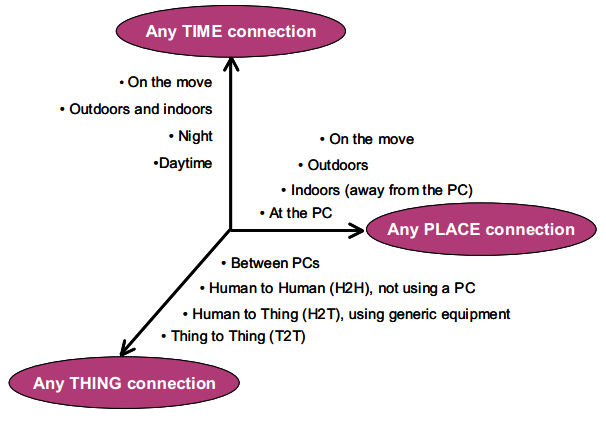
\includegraphics[width=0.85\textwidth]{eikona_07}
\caption[Μια νέα διάσταση]{Μια νέα διάσταση\cite{iot}}
\end{figure}

Το Διαδίκτυο των Πραγμάτων διαφέρει, επίσης, από τα δίκτυα αισθητήρων ή το Διαδίκτυο, αλλά είναι <<υλικά αντικείμενα που συνδέονται στο διαδίκτυο>>, που σημαίνει: πρώτον, ο πυρήνας και το θεμέλιο του ΙοΤ είναι ακόμα το Διαδίκτυο –βασίζεται στο Διαδίκτυο ως μια διεύρυνση και επέκταση του δικτύου– και δεύτερον, γίνεται διεύρυνση των πελατών του σε οποιαδήποτε πράγματα, ώστε να επιτευχθεί ανταλλαγή πληροφοριών και επικοινωνία. Ως εκ τούτου, αν και δεν υπάρχει αυστηρός ορισμός, μπορούμε να ορίσουμε το Διαδίκτυο των Πραγμάτων ως το δίκτυο που χρησιμοποιεί συσκευές ραδιοσυχνοτικής αναγνώρισης (RFID - radio frequency identification), υπέρυθρους αισθητήρες, συστήματα παγκόσμιου εντοπισμού θέσης, σαρωτές λέιζερ και άλλες αισθητήριες διατάξεις πληροφοριών, σύμφωνα με το συμφωνημένο πρωτόκολλο σε κάθε στοιχείο συνδεδεμένο στο Διαδίκτυο, για ανταλλαγή πληροφοριών και επικοινωνία, προκειμένου να επιτευχθούν έξυπνες λειτουργίες αναγνώρισης, εντοπισμού θέσης, παρακολούθησης και διαχείρισης.
\medskip

Το Διαδίκτυο των Πραγμάτων έχει τρία σημαντικά χαρακτηριστικά:
\begin{enumerate}
\item Ολοκληρωμένη αίσθηση χρησιμοποιώντας RFID τεχνολογία, αισθητήρες και δύο διαστάσεων κώδικα για τη συλλογή πληροφοριών από αντικείμενα οπουδήποτε και οποιαδήποτε στιγμή
\item Αξιόπιστη μετάδοση. Ακριβής και σε πραγματικό χρόνο παροχή πληροφοριών από τα αντικείμενα, εμπλέκοντας διάφορα τηλεπικοινωνιακά δίκτυα και το Διαδίκτυο
\item Έξυπνη επεξεργασία χρησιμοποιώντας έξυπνους τρόπους όπως το cloud computing και η ασαφής αναγνώριση (fuzzy identification) για να αναλύσει και να επεξεργαστεί τεράστιες ποσότητες δεδομένων και πληροφοριών, με σκοπό την εφαρμογή ευφυούς ελέγχου στα αντικείμενα
\end{enumerate}

\section{Κύριες Τεχνολογίες για το Διαδίκτυο των Πραγμάτων}

Το Διαδίκτυο των πραγμάτων είναι μια τεχνολογική επανάσταση που αντιπροσωπεύει το μέλλον της πληροφορικής και των επικοινωνιών και η ανάπτυξή του χρειάζεται υποστήριξη από κάποιες καινοτόμες τεχνολογίες. Μπορεί να επιτευχθεί μέσω της αλληλεπίδρασης και τελειοποίησης της τεχνολογίας ανίχνευσης σήματος, των επικοινωνιών μικρής εμβέλειας, τη μετάδοση σε μεγάλες αποστάσεις, την έξυπνη ανάλυση και τη διαχείριση. Οι μείζονος σημασίας τεχνολογίες που θα κυριαρχήσουν στις ΙοΤ εφαρμογές είναι τα ασύρματα δίκτυα αισθητήρων (WSN), η ταυτοποίηση μέσω ραδιοσυχνοτήτων (RFID) και οι κινητές επικοινωνίες μαζί με τα υπάρχοντα LAN\slash WAN δίκτυα, όπως παρουσιάζει και το σχ.~\ref{eik8}. Στην έκθεση της ΙΤU, αναφέρονται τέσσερεις καθοριστικής σημασίας εφαρμοσμένες τεχνολογίες: η RFID, οι τεχνολογίες αισθητήρων, οι έξυπνες τεχνολογίες και η νανοτεχνολογία.
\begin{figure}[!hbt]
\centering
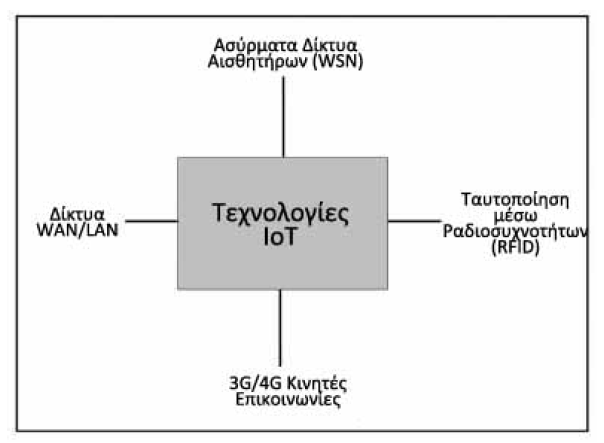
\includegraphics[height=6cm,width=10cm]{eikona_08}
\caption[Κύριες Τεχνολογίες στο IoT]{Κύριες Τεχνολογίες στο IoT\cite{zwtou}}\label{eik8}
\end{figure}

\subsection{Ταυτοποίηση μέσω ραδιoσυχνοτήτων (RFID)}

Η ταυτοποίηση μέσω ραδιοσυχνοτήτων θεωρείται από τους βασικούς μοχλούς της ανάπτυξης του Διαδικτύου των Πραγμάτων. Τα αντικείμενα θα πρέπει να προσδιορίζονται έτσι ώστε να μπορούν να συνδεθούν. Η RFID τεχνολογία, που χρησιμοποιεί ραδιοκύματα για τον προσδιορισμό των στοιχείων, μπορεί να παρέχει αυτή τη λειτουργία.

Το RFID σύστημα καλύπτει διάφορες ζώνες συχνοτήτων από τα 124 kHz ως τα 5.8 GHz, όπως 124 kHz, 135 kHz, 13.56 ΜHz, 470 ΜHz, 900 ΜHz, 2.4 GHz και 5.8 GHz. Διαφορετικές συχνότητες μπορούν να χρησιμοποιηθούν σε ποικίλες περιπτώσεις εφαρμογών. Το χαμηλής συχνότητας σύστημα RFID έχει ισχυρή δυνατότητα διείσδυσης και μπορεί να διαπεράσει σχεδόν κάθε αντικείμενο, εκτός από μέταλλο, χωρίς να επηρεάσει τη λειτουργία ανάγνωσης και γραφής. Αντίθετα, η ικανότητα διείσδυσης του RFID συστήματος υψηλής συχνότητας είναι μικρή, αλλά το εύρος μετάδοσης είναι μεγαλύτερο από το αντίστοιχο του συστήματος χαμηλής συχνότητας.

Η τεχνολογία αποτελείται από ετικέτες\slash αναμεταδότες, ένα πρόγραμμα ανάγνωσης και ένα υπολογιστικό σύστημα υποστήριξης. Η ετικέτα έχει ένα μοναδικό αναγνωριστικό (ID) και μια κεραία για να μεταδίδει\slash λαμβάνει ραδιοκύματα από τον αναγνώστη που βρίσκεται σε κοντινή απόσταση. Ο αναγνώστης διαβιβάζει πληροφορίες που έλαβε από τις ετικέτες στο σύστημα υποστήριξης για επικύρωση και το σύστημα υποστήριξης εκτελεί τις εφαρμογές σύμφωνα με τα δεδομένα που έλαβε από τον αναγνώστη. Οι RFID ετικέτες μπορεί να είναι ενεργητικές ή παθητικές. Οι ενεργητικές ετικέτες έχουν onboard παροχή ισχύος και έχουν μεγάλη εμβέλεια ανάγνωσης με ρυθμό ραδιοφάρου (beacon rate), τυπικά, από 1 ως 15 δευτερόλεπτα. Από την άλλη, οι παθητικές ετικέτες είναι φθηνές και μικρές με μικρό εύρος ανάγνωσης. Μια παθητική ετικέτα δεν έχει τροφοδοσία από μόνη της και απορροφά ενέργεια από το ηλεκτρομαγνητικό πεδίο που δημιουργεί η κεραία της συσκευής ανάγνωσης. Επίσης, υπάρχουν ημι-παθητικές και ημι-ενεργητικές ετικέτες. Μερικές φορές η τεχνολογία RFID έχει επισημανθεί ως αντικατάσταση του bar code, αλλά το RFID σύστημα μπορεί να κάνει πολύ περισσότερα από αυτό. Επιπλέον του προσδιορισμού στοιχείων, μπορεί να παρακολουθεί τα στοιχεία σε πραγματικό χρόνο για να πάρει σημαντικές πληροφορίες για την τοποθεσία και την κατάστασή τους.

Με λίγα λόγια, ένας από τους κρίσιμους παράγοντες της IoT υποδομής είναι ο προσδιορισμός τρισεκατομμυρίων αντικειμένων και η RFID παρέχει μια σημαντική τεχνολογική υποστήριξη για την απαίτηση αυτή. Συνεπώς, μια ώριμη τεχνολογία RFID παρέχει μια ισχυρή στήριξη για το Διαδίκτυο των Πραγμάτων.

\subsection{Τεχνολογία αισθητήρων}

Τα δίκτυα αισθητήρων αποτελούνται από ένα μεγάλο αριθμό μικροσκοπικών κόμβων αισθητήρων, με δυνατότητα ανίχνευσης των αντικειμένων και του περιβάλλοντος στο φυσικό κόσμο, καθώς και δυνατότητα επικοινωνίας στον ψηφιακό κόσμο των συστημάτων υπολογιστών για τη λήψη τεκμηριωμένων αποφάσεων. Οι αισθητήρες μπορούν να θεωρηθούν τα <<αισθητήρια όργανα>> του υλικού κόσμου και παρέχουν τις ακατέργαστες πληροφορίες για την επεξεργασία, τη μετάδοση, την ανάλυση και την ανατροφοδότηση πληροφοριών. Οι κόμβοι συλλέγουν και προωθούν τα δεδομένα στο σταθμό βάσης για την από κοινού παρακολούθηση των φυσικών αντικειμένων ή των περιβαλλοντικών συνθηκών, όπως η θερμοκρασία, η πίεση και η κίνηση. Στα Ασύρματα Δίκτυα Αισθητήρων (Wireless Sensor Netwroks - WSN) υπάρχουν, συνήθως, ένας ή περισσότεροι σταθμοί βάσης και αρκετοί κόμβοι αισθητήρων. Ο σταθμός βάσης λειτουργεί ως η αξιόπιστη κεντρική αρχή και, επίσης, χρησιμεύει ως επεξεργαστής δεδομένων που συνδέει το δίκτυο αισθητήρων με τον εξωτερικό κόσμο.

\subsection{Έξυπνη Τεχνολογία}

Οι έξυπνες τεχνολογίες είναι οι μέθοδοι που χρησιμοποιούνται για να επιτευχθεί συγκεκριμένος σκοπός, χρησιμοποιώντας γνώση εκ των προτέρων. Τα αντικείμενα που καθίστανται έξυπνα μετά την εμφύτευση έξυπνων τεχνολογιών μπορούν να επικοινωνούν με τους χρήστες ενεργά ή παθητικά. Το περιεχόμενο και η κατεύθυνση των σημαντικότερων ερευνών περιλαμβάνουν θεωρία τεχνητής νοημοσύνης, προηγμένες τεχνολογίες και συστήματα αλληλεπίδρασης ανθρώπου-μηχανής, έξυπνα συστήματα και τεχνολογία ελέγχου, ευφυή επεξεργασία σήματος.

\subsection{Νανοτεχνολογία}

Η νανοτεχνολογία χρησιμοποιείται για τη βελτίωση των προϊόντων σε πολλές βιομηχανίες και κλάδους, μεταξύ των οποίων η ιατρική, η ενέργεια και οι μεταφορές. Η χρήση νανοτεχνολογίας σημαίνει ότι τα αντικείμενα που αλληλεπιδρούν και συνδέονται το ένα με το άλλο μπορεί να είναι ολοένα και μικρότερα.

Πρόσφατα, η νανοτεχνολογία έχει χρησιμοποιηθεί για την ανάπτυξη ευαίσθητων υλικών υψηλής επίδοσης και νέων μεθόδων παραγωγής αισθητήρων, όπως η τεχνολογία μικροηλεκτρονικομηχανικών συστημάτων (MEMS – MicroElectroMechanical Systems) που επεκτείνει σημαντικά το πεδίο εφαρμογής των αισθητήρων στα συστήματα ηλεκτρικής ενέργειας και προωθεί την ανάπτυξη της βιομηχανίας αισθητήρων.

\section{Η Αρχιτεκτονική του Διαδικτύου των Πραγμάτων}

Το Διαδίκτυο των Πραγμάτων μπορεί να διαιρεθεί σε τρία επίπεδα: το στρώμα αντίληψης (perception layer), το στρώμα δικτύου (network layer) και το στρώμα εφαρμογής (application layer).

Το στρώμα αντίληψης αποτελείται από δύο-διαστάσεων κωδικό ετικέτας και αναγνώστη κωδικού, RFID ετικέτα και αναγνώστη, κάμερα, GPS, όλα τα είδη των αισθητήρων, δίκτυο αισθητήρων, Μ2Μ τερματικά, πύλη αισθητήρα (gateway) κ.ά. Η κύρια λειτουργία του στρώματος αντίληψης είναι η αντίληψη και ταυτοποίηση των αντικειμένων και η συλλογή πληροφοριών.

Το στρώμα δικτύου αποτελεί ένα συγκλίνον δίκτυο το οποίο σχηματίζεται από όλα τα είδη δικτύων επικοινωνιών και το διαδίκτυο. Έχει γίνει ευρέως αποδεκτό ότι αυτό το τμήμα είναι το πιο ώριμο κομμάτι. Εξάλλου, τα κέντρα διαχείρισης και πληροφοριών του ΙοΤ είναι τμήματα του στρώματος δικτύου. Το στρώμα δικτύου, δηλαδή, όχι μόνο έχει την ικανότητα της λειτουργίας δικτύου, αλλά θα πρέπει να βελτιώνει την ικανότητα της λειτουργίας πληροφοριών. Παρέχει και επεξεργάζεται πληροφορίες από τα στρώματα αντίληψης, σαν να είναι το νευρικό κέντρο και ο εγκέφαλος της δομής, ολοκληρώνοντας τη μεταφορά πληροφοριών και δεδομένων μεταξύ του στρώματος αντίληψης και του στρώματος εφαρμογής. Το στρώμα δικτύου είναι η υποδομή ώστε να γίνει το ΙοΤ καθολική υπηρεσία.

Το στρώμα εφαρμογής αποτελείται κυρίως από είδη συστημάτων εφαρμογών, με κύριες λειτουργίες τη σύγκλιση, τη μετατροπή, την ανάλυση και την ανταλλαγή δεδομένων, καθώς και τη σχετική πλατφόρμα υποστήριξης για τους χρήστες. Παράλληλα, το στρώμα αυτό προσφέρει επίσης διεπαφή εφαρμογής του διαδικτύου των πραγμάτων και υπηρεσίες εφαρμογής για τις συσκευές και τα τερματικά των χρηστών. Το στρώμα εφαρμογής είναι η τεχνολογία του Διαδικτύου των Πραγμάτων σε συνδυασμό με την τεχνογνωσία της βιομηχανίας για να επιτευχθεί μια ευρεία σειρά ευφυών λύσεων εφαρμογών. Μέσω του στρώματος αυτού, το Διαδίκτυο των Πραγμάτων μπορεί να επιτύχει, τελικά, την ενσωμάτωση της τεχνολογίας πληροφοριών με τη βιομηχανία. Θα έχει μεγάλη επίδραση στην οικονομική και κοινωνική ανάπτυξη. Το κεντρικό στοιχείο του στρώματος εφαρμογής είναι η ανταλλαγή πληροφοριών και η ασφάλεια των πληροφοριών.

Πρέπει να σημειωθεί ωστόσο, πως, επί του παρόντος, δεν υπάρχει κάποια ευρέως αποδεκτή αρχιτεκτονική του Διαδικτύου των Πραγμάτων. Η πιο αντιπροσωπευτική δομή είναι αυτή της EPC Global που υποστηρίζεται από την Ευρώπη και τις Η.Π.Α και το ιαπωνικό UID (Ubiquitous ID) IoT σύστημα.

\section{Οι γενικές εφαρμογές του IoT}

Παρότι η εφαρμογή του ΙοΤ είναι ακόμα σε πρώιμο στάδιο, έχει σημειώσει επιτυχία σε ορισμένους τομείς. Προς το παρόν, η εφαρμογή του επικεντρώνεται κυρίως στην υλικοτεχνική υποδομή, σε στρατιωτικά θέματα, στην παρακολούθηση και τη διαχείριση, στην ιατρική φροντίδα κ.ά.

Σύμφωνα με τα ίδια τα χαρακτηριστικά του, θα πρέπει να παρέχονται οι ακόλουθες κατηγορίες υπηρεσιών:
\begin{enumerate}
\item Υπηρεσία Δικτύωσης: αναγνώριση\slash ταυτοποίηση, επικοινωνία και τοποθέτηση αγαθών
\item Πληροφοριακή Υπηρεσία: συλλογή, αποθήκευση και αναζήτηση πληροφοριών
\item Υπηρεσία Λειτουργίας: απομακρυσμένη ρύθμιση παραμέτρων, παρακολούθηση, λειτουργία και έλεγχος
\item Υπηρεσία Ασφάλειας: διαχείριση χρηστών, έλεγχος πρόσβασης, εκδήλωση συναγερμού, ανίχνευση εισβολής, πρόληψη επιθέσεων
\item Υπηρεσία Διαχείρισης: διάγνωση βλαβών, βελτιστοποίηση απόδοσης, αναβαθμίσεις του συστήματος, υπηρεσίες διαχείρισης της τιμολόγησης
\end{enumerate}
\clearpage
Ο γενικός τύπος υπηρεσιών του IoT που αναφέρθηκαν μπορούν να επεκταθούν βάσει των απαιτήσεων της εκάστοτε εφαρμογής του στους διάφορους τομείς. Στο σχ.~\ref{eik9} φαίνονται τα μελλοντικά πλαίσια χρήσης του ΙοΤ.
\begin{figure}[!ht]
\centering
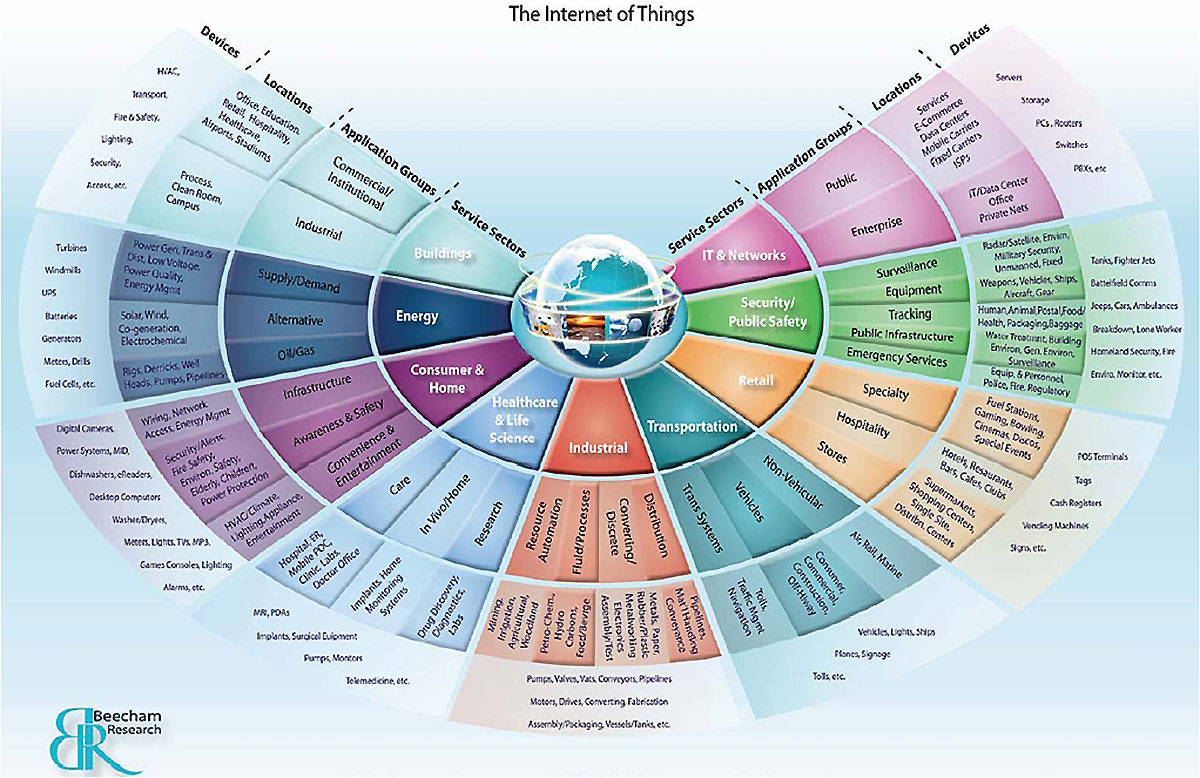
\includegraphics[width=\textwidth]{eikona_09}
\caption[Σενάρια εφαρμογής του IoT]{Σενάρια εφαρμογής του IoT\cite{cisco}}\label{eik9}
\end{figure}

\section{Οι εφαρμογές του IoT στο Έξυπνο Δίκτυο}

Τα συστήματα ηλεκτρικής ενέργειας περιλαμβάνουν τρία σημαντικά υποσυστήματα, την παραγωγή ηλεκτρικής ενέργειας, τη διανομή ενέργειας και τη χρησιμοποίησή της. Πρόσφατα, το Διαδίκτυο των πραγμάτων έχει ευρέως αναγνωριστεί ως μια υποσχόμενη τεχνολογία που μπορεί να ενισχύσει όλα αυτά τα υποσυστήματα, γεγονός που το καθιστά βασική συνιστώσα των επόμενης γενιάς συστημάτων ηλεκτρικής ενέργειας, των έξυπνων δικτύων.

Τα κύρια σενάρια εφαρμογής του IoT στα έξυπνα δίκτυα είναι:
\begin{itemize}
\item Στον τομέα της παραγωγής ενέργειας , το ΙοΤ μπορεί να χρησιμοποιηθεί για την παρακολούθηση της μονάδας, των κατανεμημένων σταθμών ηλεκτροπαραγωγής, της περιοχής των σταθμών παραγωγής, των ρύπων και των εκπομπών αερίων, της ενεργειακής κατανάλωσης, του υλικού του άνθρακα, της αιολικής μονάδας παραγωγής, των φωτοβολταϊκών σταθμών παραγωγής, της παραγωγής ηλεκτρικής ενέργειας από βιομάζα, της αποθήκευσης ενέργειας, της διασύνδεσης ηλεκτρικής ενέργειας κτλ.
\item Το ΙοΤ επίσης χρησιμοποιείται ευρέως για την παρακολούθηση των γραμμών μεταφοράς, για την προστασία των πύργων, για έξυπνους υποσταθμούς, για την αυτοματοποίηση της διανομής, για την παρακολούθηση της κατάστασης διανομής, για τη διαχείριση της λειτουργίας και του εξοπλισμού.
\item Το ΙοΤ χρησιμοποιείται κυρίως για τους έξυπνους μετρητές και τη μέτρηση κατανάλωσης ενέργειας, τη σύγκλιση του πολύ-δικτύου, για τα ηλεκτρικά οχήματα και τη φόρτισή τους, για την παρακολούθηση και διαχείριση της ενεργειακής απόδοσης, για τη διαχείριση ζήτησης (DSM), κ.ά.
\end{itemize}

\begin{figure}[!hb]
\centering
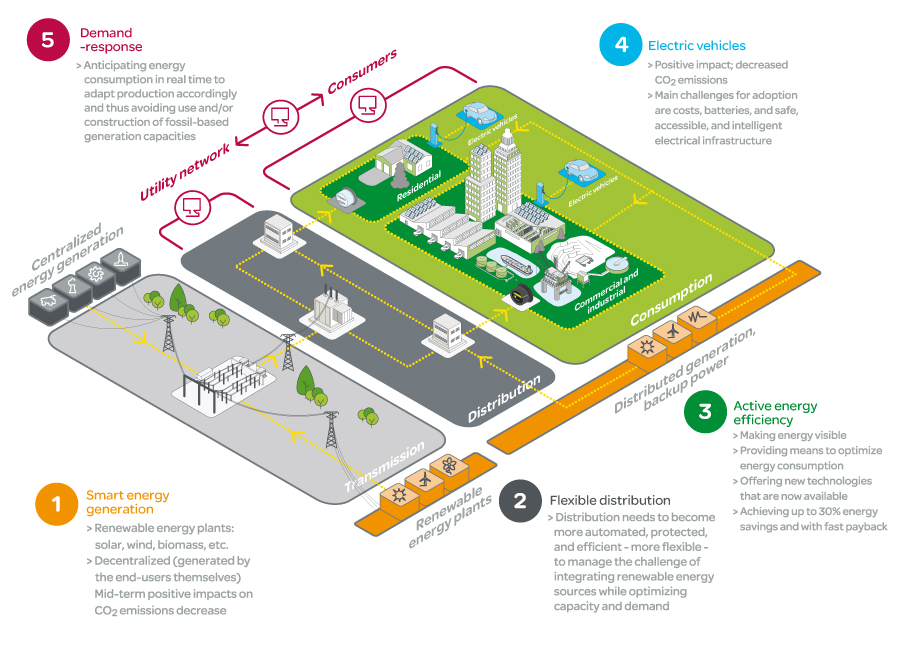
\includegraphics[width=0.9\textwidth]{eikona_10}
\caption[Η δομή του ΙοΤ εφαρμοσμένη στο Έξυπνο Δίκτυο]{Η δομή του ΙοΤ εφαρμοσμένη στο Έξυπνο Δίκτυο\cite{schneider}}
\end{figure}

\chapter{Συσκευές μέτρησης και δίκτυο ZigBee}
\section{Συσκευές Μέτρησης}

H Meazon Α.Ε. παράγει δύο ειδών μετρητικές συσκευές, οι οποίες συνδέονται σε δίκτυο ZigBee για τη μεταφορά των μετρητικών τους δεδομένων. Υπάρχει ο μονοφασικός μετρητής που ονομάζεται Bizy Plug (σχ.~\ref{eik11}) και ο τριφασικός μετρητής που ονομάζεται DinRail Basic (σχ.~\ref{eik12}). 
\begin{figure}[!ht]
\centering
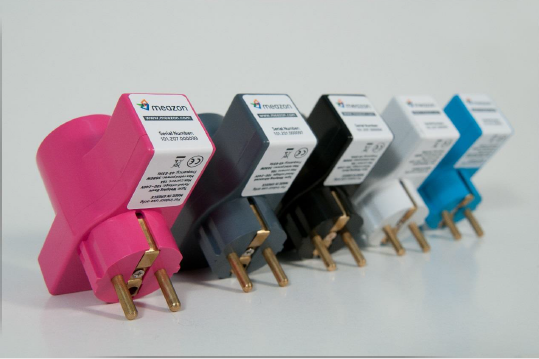
\includegraphics[width=0.88\textwidth]{eikona_11}
\caption[Μονοφασικός μετρητής - Bizy Plug]{Μονοφασικός μετρητής - Bizy Plug\cite{biz}}\label{eik11}
\end{figure}

\begin{figure}[!tb]
\centering
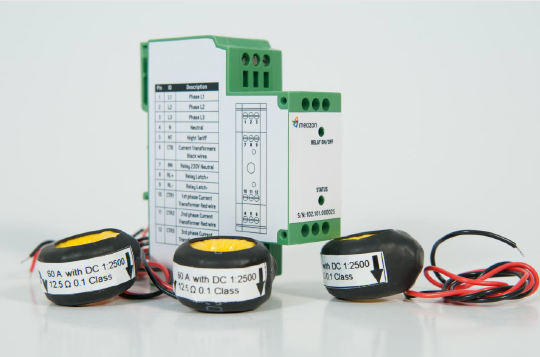
\includegraphics[width=0.88\textwidth]{eikona_12}
\caption[Τριφασικός μετρητής - DinRail Basic]{Τριφασικός μετρητής - DinRail Basic\cite{din}}\label{eik12}
\end{figure}

Ο τριφασικός μετρητής συνδέεται απευθείας στον ηλεκτρικό πίνακα του κτιρίου και μετρά την κατανάλωση ενέργειας τριών φάσεων ή τριών ηλεκτρικών γραμμών, ενώ ο μονοφασικός μετρητής συνδέεται μεταξύ της πρίζας και της ηλεκτρικής συσκευής που θέλουμε να μετρήσουμε και μετρά την κατανάλωση της συσκευής που έχουμε συνδέσει. Ο μονοφασικός μετρητής έχει και ενσωματωμένο ρελέ, οπότε μπορούμε να ελέγχουμε και την κατάσταση στην οποία θα βρίσκεται η συσκευή που έχουμε συνδέσει (on\slash of\mbox{}f). Επίσης, διαθέτει και αισθητήρα μέτρησης θερμοκρασίας για να μας παρέχει πληροφορία για τη θερμοκρασία του χώρου που βρίσκεται. Το μέγιστο ρεύμα φορτίου που μπορούν να δεχθούν οι μετρητές είναι 60~A ανά φάση\slash γραμμή για τον τριφασικό μετρητή και 16~A για το μονοφασικό. Σύμφωνα με τα στοιχεία της εταιρείας, η ακρίβεια των μετρητών είναι μικρότερη του 1\% \cite{biz,din}.

Οι μετρητές παίρνουν μέτρηση σε μικρά διαστήματα (μέχρι και ένα δευτερόλεπτο) και μέσω μιας συσκευής USB (PAN Coordinator) στέλνουν στο BeagleBone ένα πακέτο με πληροφορίες. Το πακέτο αυτό είναι της μορφής JSON και περιέχει τα κατάλληλα δεδομένα ώστε να μπορέσει το BeagleBone να εξάγει αποτελέσματα για τις εξής ποσότητες μεταξύ άλλων: στιγμιαία κατανάλωση ενέργειας, θερμοκρασία του χώρου της πρίζας (για το μονοφασικό μετρητή), ID του μετρητή, καθώς και τη συνολική μέτρηση ενέργειας από την πρώτη χρήση του μετρητή. Η προκαθορισμένη επιλογή είναι, ανά διαστήματα των 5 λεπτών, να στέλνονται τα μετρητικά δεδομένα μέσω του BeagleBone στο Cloud της Meazon. Για την αποστολή των μετρήσεων θα πρέπει το BeagleBone να έχει πρόσβαση στο Internet. Εάν για κάποιο λόγο δεν είναι δυνατή η πρόσβαση τη χρονική στιγμή που είναι προγραμματισμένη η αποστολή των δεδομένων στο Cloud, το BeagleBone έχει τη δυνατότητα να στείλει ετεροχρονισμένα τις μετρήσεις που δεν έχουν σταλεί, καθώς μπορεί και κρατά ιστορικό.

\section{Το πρωτόκολλο ZigBee}

\subsection{Τι είναι το ZigBee}

Το ZigBee είναι ένα πρότυπο που καθορίζει ένα σύνολο από πρωτόκολλα επικοινωνίας για χαμηλού ρυθμού μετάδοση δεδομένων, μικρής εμβέλειας ασύρματων δικτύων. Οι ασύρματες συσκευές βασισμένες στο πρότυπο του ZigBee λειτουργούν στις ζώνες συχνοτήτων 868 MHz, 915 MHz και 2.4 GHz. Ο μέγιστος ρυθμός μετάδοσης δεδομένων είναι 250 Kbits ανά δευτερόλεπτο. Το ZigBee χρησιμοποιείται ως επί το πλείστον σε εφαρμογές όπου απαιτούνται μπαταρίες για τη λειτουργία τους και μερικές από τις κύριες απαιτήσεις είναι ο χαμηλός ρυθμός μετάδοσης δεδομένων, το χαμηλό κόστος, και η μεγάλη διάρκεια ζωής της μπαταρίας. Σε πολλές εφαρμογές του ZigBee, ο συνολικός χρόνος που κάθε μία από τις ασύρματες συσκευές συμμετέχει σε κάθε είδους δραστηριότητα στο δίκτυο είναι πολύ περιορισμένος. Η συσκευή καταναλώνει το μεγαλύτερο διάστημά της βρισκόμενη σε κατάσταση αδράνειας (power-saving mode), που είναι γνωστή και ως ``sleep mode''. Ως εκ τούτου, παρουσιάζει πολύ μικρή κατανάλωση ενέργειας.

Το πρότυπο του ZigBee (ZigBee standard) αναπτύσσεται από τη ``συμμαχία'' ZigBee (the ZigBee Alliance), που συμπεριλαμβάνει εκατοντάδες επιχειρήσεις, από παραγωγούς ημιαγωγών έως και κατασκευαστές λογισμικού για παραγωγή πρωτότυπου εξοπλισμού (OEMs) και εγκαταστάτες. Η ZigBee Alliance σχηματίστηκε το 2002 σαν ένας μη κερδοσκοπικός οργανισμός, ανοιχτή σε οποιονδήποτε επιθυμεί να συμμετάσχει στο εγχείρημα. Το πρότυπο ZigBee υιοθέτησε το πρότυπο του IEEE 802.15.4 σαν το φυσικό επίπεδο διεπαφής (Physical Layer, PHY) και σαν Μέσο Πρόσβασης Ελέγχου (Medium Access Control, MAC). Όπως γίνεται κατανοητό από τα παραπάνω, κάθε συσκευή συμβατή με το ZigBee είναι συμβατή επίσης και με το πρότυπο IEEE 802.15.4.

Το πρότυπο ZigBee συμβάλλει στη μείωση του κόστους εγκατάστασης, με την απλοποίηση των πρωτοκόλλων επικοινωνίας και με τη μείωση του ρυθμού δεδομένων. Οι ελάχιστες απαιτήσεις που ικανοποιούν τα πρότυπα ZigBee και IEEE 802.15.4 είναι σχετικά ``χαλαρές'' αν τις συγκρίνουμε με άλλα πρότυπα, όπως το IEEE 802.11, με αποτέλεσμα να μειώνεται η πολυπλοκότητα και το κόστος εγκατάστασης πομποδεκτών συμβατών με το ZigBee.

Ο ``κύκλος καθηκόντων'' (duty cycle) είναι ο λόγος του χρόνου που μια συσκευή είναι ενεργή στο δίκτυο, προς το συνολικό χρόνο που αυτή λειτουργεί, είτε αυτή είναι ενεργή είτε σε ``sleep mode''. Για παράδειγμα, αν μια συσκευή ενεργοποιείται κάθε λεπτό και μένει ενεργή για 60ms, τότε ο ``κύκλος καθηκόντων'' της συγκεκριμένης συσκευής είναι 0.001, ή 0.1\%. Στις περισσότερες εφαρμογές τύπου ZigBee, οι συσκευές έχουν ``κύκλους καθηκόντων'' μικρότερους από 1\%, ώστε να εξασφαλίσουν πολύ μικρή κατανάλωση ενέργειας.

\subsection{ZigBee εναντίον Bluetooth και IEEE 802.11}

Συγκρίνοντας το πρότυπο του ZigBee με αυτά των Bluetooth και IEEE 802.11 WLAN, μας βοηθάει στο να κατανοήσουμε πώς το ZigBee διαφοροποιείται από τα ήδη υπάρχοντα αυτά πρότυπα. Το σχ.~\ref{eik13} συγκεντρώνει τα βασικά χαρακτηριστικά αυτών των τριών προτύπων.
%\clearpage
%\begin{figure}[ht]
%\centering
%\includegraphics[height=10cm]{graph}
%\caption{Συγκρίνοντας το ZigBee με το Bluetooth και το IEEE 802.11}\label{eik13}
%\end{figure}

\begin{table}[!hb]
\centering
%{\renewcommand{\arraystretch}{1.5}
%\renewcommand{\tabcolsep}{0.2cm}
\begin{tabular}{!{\vrule width .1em} C{3cm}| C{4cm}| C{2cm}| C{2.5cm}!{\vrule width .1em}}
\specialrule{.1em}{.05em}{0em}
 & \textbf{ZigBee} & \textbf{IEEE 802.11\newline(wi-f\mbox{}i)} & \textbf{Bluetooth}\\ \specialrule{.1em}{0em}{0em}
\textbf{Ρυθμός μετάδοσης} & 20,40 και 250 Kbps & 11 \& 54 Mbps & 1 Mbps\\ \hline
\textbf{Εμβέλεια} & 10-100 m & 50-100 m & 10 m\\ \hline
\textbf{Συχνότητα λειτουργίας} & 868 MHz(EU),\newline 900-928 MHz(NA),\newline2.4 GHz(παγκόσμια) & 2.4 και 5 GHz & 2.4 GHz\\ \hline
\textbf{Πολυπλοκότητα} & Χαμηλή & Υψηλή & Υψηλή\\ \hline
\textbf{Κατανάλωση ενέργειας} & Πολύ χαμηλή (στόχος σχεδιασμού) & Υψηλή & Μέση\\ \hline
\textbf{Μια συσκευή συνδέεται στο δίκτυο σε..} & Λιγότερο από 30ms & 3-5s & Μέχρι και 10s\\ 
\specialrule{.1em}{0em}{.05em}
\end{tabular}
%}
\caption[Συγκρίνοντας ZigBee, Bluetooth και IEEE 802.11]{Συγκρίνοντας το ZigBee με το Bluetooth και το IEEE 802.11}\label{eik13}
\end{table}
\clearpage
Το πρότυπο IEE 802.11 είναι μια ``οικογένεια'' προτύπων. Το IEEE 802.11 επιλέγεται εδώ επειδή λειτουργεί στη ζώνη συχνοτήτων 2.4GHz, που είναι και η συνήθης ζώνη για το Bluetooth και το ZigBee. Το ΙΕΕΕ 802.11 έχει έναν υψηλό ρυθμό μετάδοσης δεδομένων (μέχρι 54Mbps), και η παροχή μίας ασύρματης σύνδεσης στο διαδίκτυο είναι μία από τις τυπικές εφαρμογές του. Η περιοχή εμβέλειάς του είναι τυπικά γύρω στα 50 με 100 μέτρα. Το Bluetooth, από την άλλη μεριά, έχει μικρότερο ρυθμό μετάδοσης δεδομένων και η περιοχή εμβέλειάς του είναι τυπικά γύρω στα 2 με 10 μέτρα. Μια διάσημη εφαρμογή του Bluetooth είναι η επικοινωνία μεταξύ ενός κινητού τηλεφώνου και ενός σετ από ``hands-free''. Το ZigBee έχει το μικρότερο ρυθμό μετάδοσης δεδομένων αλλά και τη μικρότερη πολυπλοκότητα μεταξύ αυτών των τριών προτύπων και παρέχει σημαντικά μεγαλύτερη διάρκεια ζωής στη μπαταρία.

Ο χαμηλός ρυθμός μετάδοσης δεδομένων του ZigBee σημαίνει ότι δεν είναι η βέλτιστη επιλογή για την υλοποίηση μιας ασύρματης σύνδεσης στο διαδίκτυο ή ενός ασύρματου ``hands-free'' με ποιότητα φωνής αντίστοιχη αυτής του CD όπου ταχύτητες μεγαλύτερες από 1Mbps απαιτούνται. Ωστόσο, αν ο στόχος της ασύρματης επικοινωνίας είναι να στέλνονται και να λαμβάνονται απλές εντολές ή συγκέντρωση πληροφοριών από αισθητήρες όπως θερμοκρασίας, υγρασίας, κ.λπ., τότε το ZigBee είναι αυτό που προσφέρει τη μεγαλύτερη ισχύ και την πιο οικονομική λύση συγκριτικά με το Bluetooth και το IEEE 802.11.

\subsection[IEEE 802.15.15 και Τεχνολογία ZigBee]{Το πρότυπο IEEE 802.15.14 και η τεχνολογία ZigBee}

Η στοίβα πρωτοκόλλων του ZigBee αποτελείται από 4 επίπεδα. Κάθε επίπεδο εκτελεί ένα συγκεκριμένο σύνολο λειτουργιών και παρέχει τις υπηρεσίες του στο ανώτερο επίπεδο μέσω μιας διεπαφής που ονομάζεται σημείο πρόσβασης υπηρεσιών ( service access point, SAP). Τα 4 επίπεδα της στοίβας πρωτοκόλλων του ZigBee είναι τα παρακάτω: 
\begin{enumerate}
\item \textbf{Το φυσικό επίπεδο (Physical layer, PHY)}. Είναι υπεύθυνο για την ενεργοποίηση και απενεργοποίηση του πομποδέκτη, μετάδοση και λήψη δεδομένων, ανίχνευση ενέργειας στο κανάλι, εκτίμηση της κατάστασης των καναλιών για την πολλαπλή πρόσβαση με ανίχνευση φέροντος και με αποφυγή συγκρούσεων (CSMA-CA) και τη μέτρηση της ποιότητας των λαμβανόμενων πακέτων.
\item \textbf{Το επίπεδο ελέγχου πρόσβασης στο μέσο (Medium Access Control layer, MAC)}. Παρέχει υπηρεσίες μεταφοράς δεδομένων και διαχείρισης. Είναι υπεύθυνο για την πρόσβαση στο κανάλι, για τη διαχείριση των χρονοσχισμών και για την παροχή μιας αξιόπιστης σύνδεσης μεταξύ δύο επιπέδων MAC. Επιπρόσθετα παρέχει τα μέσα για την εφαρμογή διαφόρων μηχανισμών ασφάλειας.
\item \textbf{Το επίπεδο δικτύου (Network layer, NWK)}. Είναι υπεύθυνο για τη δημιουργία του δικτύου, για την είσοδο και την έξοδο μιας συσκευής από ένα δίκτυο, για την ασφάλεια και για τη δρομολόγηση των μεταδιδόμενων πακέτων.
\item \textbf{Το επίπεδο εφαρμογών (Application layer, APL)}. Περιλαμβάνει το υποεπίπεδο υποστήριξης εφαρμογών (Application support sublayer, APS), το πλαίσιο εφαρμογών (Application framework, AF), τα αντικείμενα συσκευής ZigBee (ZigBee Device Objects, ZDO) και τις καθορισμένες από τον κατασκευαστή εφαρμογές. Το υποεπίπεδο APS είναι υπεύθυνο για τη σύνδεση δύο συσκευών βάσει των αναγκών και των υπηρεσιών τους και για την αποστολή δεδομένων μεταξύ τους. Τα ZDO είναι αυτά που καθορίζουν το ρόλο της κάθε συσκευής στο δίκτυο και το επίπεδο ασφάλειας. Επίσης συμβάλλουν στην ανίχνευση των συσκευών σε ένα δίκτυο και στον προσδιορισμό των υπηρεσιών που αυτές παρέχουν. Το πλαίσιο εφαρμογών είναι το περιβάλλον στο οποίο φιλοξενούνται οι εφαρμογές μέσα σε μία συσκευή ZigBee.
\end{enumerate}

Όπως φαίνεται και στο σχ.~\ref{eik14}, τα πρώτα δύο επίπεδα καθορίζονται από το πρότυπο IEEE 802.15.4. Αυτό το πρότυπο αναπτύχθηκε από την επιτροπή IEEE 802 και ξεκίνησε επισήμως το 2003. Το IEEE 802.15.4 ορίζει τις απαιτήσεις για τα επίπεδα PHY και MAC της ασύρματης δικτύωσης, αλλά δεν καθορίζει τις απαιτήσεις για τα πρωτόκολλα που βρίσκονται σε υψηλότερο επίπεδο. Το πρότυπο ZigBee ορίζει μόνο τα επίπεδα της δικτύωσης, της εφαρμογής, και της ασφάλειας, ενώ υιοθετεί τα επίπεδα IEEE 802.15.4 PHY και MAC σαν υποσύνολο του ευρύτερου δικτυακού πρωτόκολλου.
\begin{figure}[!ht]
\centering
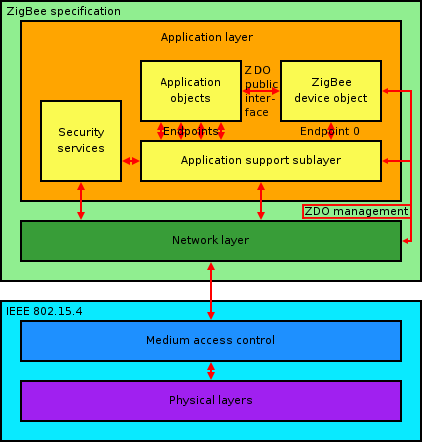
\includegraphics{eikona_14}
\caption[Επίπεδα δικτύου του ZigBee (networking layers)]{Επίπεδα δικτύου του ZigBee (networking layers)\cite{zigbee}}\label{eik14}
\end{figure}

\subsection{Συχνότητα λειτουργίας και ρυθμός μετάδοσης δεδομένων}

Υπάρχουν τρεις ζώνες συχνοτήτων στην τελευταία έκδοση του IEEE 802.15.4, που εκδόθηκε το Σεπτέμβριο του 2006:
\begin{itemize}
\item 868-868.6MHz (868MHz band)
\item 902-928MHz (915MHz band)
\item 2400-2483.5MHz (2.4GHz band)
\end{itemize}

Η ζώνη των 868 MHz χρησιμοποιείται στην Ευρώπη για μια σειρά από εφαρμογές, όπως αυτές των ασύρματων δικτύων μικρής εμβέλειας. Οι άλλες δύο ζώνες (915 MHz και 2.4 GHz) είναι μέρος των βιομηχανικών, επιστημονικών και ιατρικών (ISM) συχνοτήτων. Η ζώνη των 915 MHz χρησιμοποιείται κυρίως στη Βόρεια Αμερική, ενώ η ζώνη των 2.4 GHz χρησιμοποιείται παγκοσμίως.

Οι μετρητικές συσκευές της Meazon χρησιμοποιούν τη ζώνη των 2.4 GHz και ο ρυθμός μετάδοσης φθάνει τα 250 Kbits/sec.

\subsection{Τύποι και ρόλοι συσκευών}

Σε ένα ασύρματο δίκτυο βασισμένο στο πρωτόκολλο IEEE 802.15.4, υπάρχουν δύο τύποι συσκευών: οι συσκευές πλήρους λειτουργίας (full-function devices, FFDs) και οι συσκευές περιορισμένης λειτουργίας (re\-duced-function devices, RFDs). 

Οι συσκευές FFD υλοποιούν κόμβους αυξημένων αρμοδιοτήτων με μεγαλύτερη υπολογιστική ικανότητα. Είναι δυνατό να χρησιμοποιούνται ως συντονιστές (coordinators) ή δρομολογητές (routers) του δικτύου καθώς έχουν τη δυνατότητα να ``μιλούν'' με όλους τους τύπους διατάξεων στο δίκτυο.

Οι συσκευές RFD, σε αντίθεση με τις FFD εμφανίζουν περιορισμένες υπολογιστικές ικανότητες και ως εκ τούτου αναλαμβάνουν απλές λειτουργίες, για τις οποίες δεν απαιτείται διακίνηση μεγάλου όγκου δεδομένων. Οι συσκευές αυτές έχουν τη δυνατότητα να ``μιλήσουν'' μόνο με συσκευές FFD.

Σε ένα δίκτυο IEEE 802.15.4, μία συσκευή FFD μπορεί να έχει τρεις διαφορετικούς ρόλους: συντονιστή, PAN (Personal Area Network) συντονιστή, και συσκευής. Ο συντονιστής (coordinator) είναι μια FFD συσκευή που έχει τη δυνατότητα να αναμεταδίδει μηνύματα. Εάν ο συντονιστής είναι επίσης ο κύριος ελεγκτής ενός προσωπικού δικτύου (PAN), τότε αποκαλείται PAN συντονιστής (PAN coordinator). Εάν μία συσκευή δε λειτουργεί ως συντονιστής, τότε απλώς καλείται συσκευή.

Το πρότυπο ZigBee χρησιμοποιεί ελαχίστως διαφοροποιημένη ορολογία, η οποία παρουσιάζεται στο σχ.~\ref{eik15}. 
\begin{figure}[!ht]
\centering
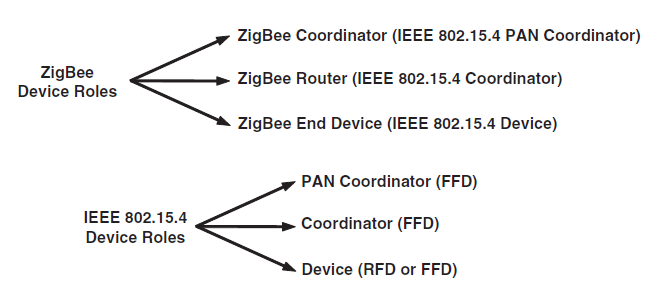
\includegraphics[width=0.93\textwidth]{eikona_15}
\caption[Ρόλοι συσκευών στα IEEE 802.15.4 και ZigBee]{Ρόλοι συσκευών στα πρότυπα IEEE 802.15.4 και ZigBee\cite{zigarrows}}\label{eik15}
\end{figure}

Ένας συντονιστής ZigBee είναι ο αντίστοιχος IEEE 802.15.4 PAN coordinator. Αναλόγως, ένας δρομολογητής ZigBee (ZigBee router) είναι μια συσκευή που μπορεί να λειτουργήσει ως ένας IEEE 802.15.4 συντονιστής. Τελικώς, μία τερματική συσκευή ZigBee (ZigBee end device), είναι μια συσκευή που δεν είναι ούτε συντονιστής ούτε δρομολογητής.

\subsection{Τοπολογίες δικτύου}

Το επίπεδο δικτύου του ZigBee υποστηρίζει τις εξής τρεις τοπολογίες δικτύου: τοπολογία αστέρα (star), πλέγματος (mesh) και συστάδας δένδρου (cluster tree).
\begin{figure}[hb]
\centering
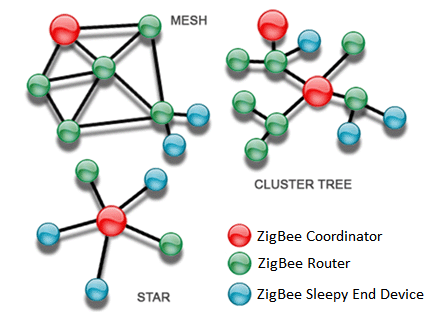
\includegraphics[width=0.8\textwidth]{eikona_16}
\caption[Υποστηριζόμενες τοπολογίες τεχνολογίας ZigBee]{Υποστηριζόμενες τοπολογίες τεχνολογίας ZigBee\cite{zig2}}\label{eik16}
\end{figure}

Η τοπολογία που χρησιμοποιείται από τη Meazon είναι αυτή του πλέγματος. Σε αυτήν την τοπολογία, που αναφέρεται και σαν peer-to-peer, υπάρχει ένας συντονιστής ΡΑΝ. Σε αντίθεση με την τοπολογία αστέρα, κάθε τερματική συσκευή μπορεί να επικοινωνήσει με κάθε άλλη συσκευή, αρκεί να είναι η μία στην εμβέλεια της άλλης. Ένα δίκτυο πλέγματος μπορεί να είναι ad hoc, να αυτο-οργανώνεται (self-organizing) και να αυτο-επουλώνεται
(self-healing). Επίσης, επιτρέπει πολλαπλά άλματα (multi-hops) για τη
δρομολόγηση μηνυμάτων από οποιαδήποτε συσκευή σε οποιαδήποτε άλλη
συσκευή στο δίκτυο. Παρέχει μεγάλη αξιοπιστία λόγω της δρομολόγησης πολλαπλής διαδρομής.\clearpage

Η τοπολογία πλέγματος έχει τα ακόλουθα χαρακτηριστικά:
\begin{itemize}
\item Τα πακέτα πραγματοποιούν πολλαπλά άλματα προκειμένου να φτάσουν στον προορισμό τους.
\item Η περιοχή του δικτύου μπορεί να αυξηθεί προσθέτοντας επιπλέον συσκευές στο δίκτυο.
\item Ελαχιστοποιεί τις νεκρές ζώνες.
\item Προσφέρει αυτο-επούλωση, που σημαίνει πως εάν κατά τη διάρκεια της μετάδοσης δε μπορεί να επιτευχθεί κάποιο μονοπάτι, ο κόμβος θα βρει εναλλακτικό μονοπάτι προς τον προορισμό.
\item Οι συσκευές μπορούν να είναι κοντά η μία στην άλλη, οπότε χρησιμοποιούν λιγότερη ισχύ.
\item Εύκολη προσθήκη και αφαίρεση συσκευών.
\item Κάθε συσκευή προέλευσης μπορεί να επικοινωνήσει με κάθε συσκευή
προορισμού.
\end{itemize}

Στο σχ.~\ref{eik17} απεικονίζεται ο USB PAN Coordinator που χρησιμοποιείται από τη Meazon για τον έλεγχο των μετρητών.
\begin{figure}[!hb]
\centering
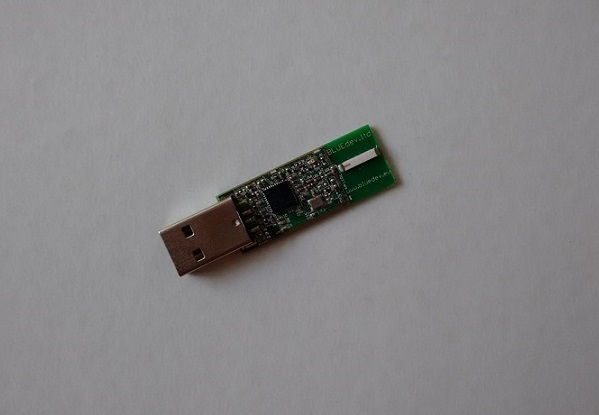
\includegraphics[scale=0.5]{eikona_17}
\caption{Φωτογραφία του PAN Coordinator}\label{eik17}
\end{figure}

\chapter{Το BeagleBone Black}

\section{Ο ρόλος του BeagleBone}

Στη θύρα USB του BeagleBone συνδέεται ο PAN Coordinator της Meazon που ``μιλά'' με τους μετρητές. Το BeagleBone τρέχει το λογισμικό που έχει γραφτεί στη Meazon και είναι υπεύθυνο για τον προγραμματισμό (scheduling) και τον έλεγχο (control) των μετρητών, καθώς και για την αποστολή των μετρητικών τους δεδομένων στο Cloud.
Το BeagleBone είναι η πύλη (gateway) για να επικοινωνήσει ο τελικός χρήστης και το cloud με τους μετρητές και τα δεδομένα που αυτοί καταγράφουν, επομένως είναι ένα νευραλγικό στοιχείο του πακέτου που προσφέρει η Meazon.
\begin{figure}[!h]
\centering
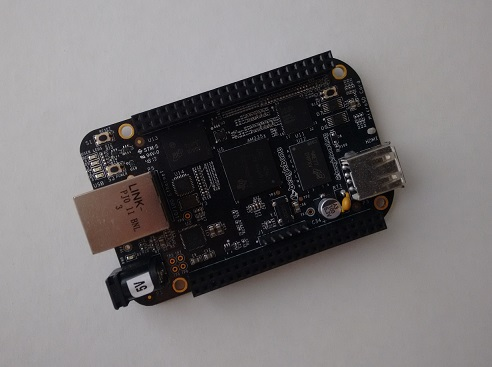
\includegraphics[scale=0.54]{eikona_18}
\caption{Φωτογραφία του BeagleBone που χρησιμοποιήθηκε}
\end{figure}

\section{Εισαγωγή στην πλατφόρμα}

Το BeagleBone Black είναι μια συμπαγής, χαμηλού κόστους υπολογιστική πλατφόρμα ανοικτού κώδικα Linux η οποία μπορεί να χρησιμοποιηθεί για να κατασκευάσουμε πολύπλοκες εφαρμογές που διασυνδέουν λογισμικό υψηλού επιπέδου με ηλεκτρονικά κυκλώματα χαμηλού επιπέδου. Είναι μια ιδανική πλατφόρμα για να κατασκευάσουμε πρωτότυπα από projects ή σχέδια προϊόντων που εκμεταλλεύονται τη δύναμη και την ελευθερία του Linux, συνδυασμένη με την άμεση πρόσβαση σε pins και διαύλους (buses) εισόδου\slash εξόδου (input\slash output), δίνοντάς μας τη δυνατότητα να αλληλεπιδράσουμε με ηλεκτρονικά εξαρτήματα, μονάδες και συσκευές USB. Τα χαρακτηριστικά της πλατφόρμας BeagleBone Black είναι ότι
\begin{itemize}
\item[\textbf{--}] είναι ισχυρή, καθώς περιέχει έναν επεξεργαστή ο οποίος μπορεί να πραγματοποιήσει μέχρι και 2 δισεκατομμύρια εντολές ανά δευτερόλεπτο,
\item[\textbf{--}] είναι χαμηλού κόστους, διαθέσιμη από \$45-\$55,
\item[\textbf{--}] υποστηρίζει πολλά τυποποιημένα interfaces για ηλεκτρονικές συσκευές,
\item[\textbf{--}] καταναλώνει λίγη ενέργεια, κυμαινόμενη μεταξύ 1~W (σε αδράνεια) και 2.3~W (μέγιστο),
\item[\textbf{--}] είναι επεκτάσιμη μέσω της χρήσης θυγατρικών πλακετών και συσκευών USB,
\item[\textbf{--}] υποστηρίζεται από μια τεράστια κοινότητα καινοτομιστών και θιασωτών, και 
\item[\textbf{--}] είναι ανοικτού υλικού και υποστηρίζει εργαλεία και εφαρμογές ανοικτού κώδικα.
\end{itemize}

Το BeagleBone ``τρέχει'' το λειτουργικό σύστημα Linux, πράγμα που σημαίνει πως μπορούμε να χρησιμοποιήσουμε πολλές βιβλιοθήκες και εφαρμογές ανοικτού κώδικα απευθείας μαζί του. Έρχεται με προεγκατεστημένη τη διανομή \textenglish{Linux \AA ngstr\"om}, αλλά στη Meazon του εγκαθιστούμε μια διανομή Ubuntu. Η διαθεσιμότητα οδηγών λογισμικού ανοικτού κώδικα μας δίνει επίσης τη δυνατότητα να διασυνδέσουμε συσκευές όπως USB κάμερες, πληκτρολόγια και προσαρμογείς Wi-Fi με το project μας, χωρίς να πρέπει να προμηθευτούμε ιδιόκτητες εναλλακτικές. Έτσι, έχουμε πρόσβαση σε εκτενείς βιβλιοθήκες κώδικα που έχουν κατασκευασθεί από μια ταλαντούχα κοινότητα ανοικτού κώδικα. Είναι όμως σημαντικό να τονίσουμε πως ο κώδικας αυτός συνήθως δεν παρέχει κάποιου είδους ασφάλεια ή εγγύηση. Εάν υπάρξουν προβλήματα, θα πρέπει να βασιστούμε στην καλή θέληση της κοινότητας για την επίλυσή τους.

Η πλατφόρμα BeagleBone σχηματίζεται από την ενσωμάτωση ενός μικροεπεξεργαστή υψηλών επιδόσεων σε μια πλακέτα τυπωμένου κυκλώματος (PCB) και σε ένα εκτενές οικοσύστημα λογισμικού. Το ίδιο το PCB δεν είναι ένα ολοκληρωμένο προϊόν, είναι περισσότερο ένα σχέδιο αναφοράς πρωτοτύπου το οποίο μπορούμε να χρησιμοποιήσουμε για να φτιάξουμε ένα ολοκληρωμένο προϊόν. Είναι μια πλατφόρμα ανοικτού υλικού, που σημαίνει πως μπορούμε να κατεβάσουμε και να χρησιμοποιήσουμε τις σχηματικές αναπαραστάσεις του υλικού και του σχεδίου του BeagleBone απευθείας μέσα στο σχέδιο του προϊόντος μας. Στην πραγματικότητα, παρά την εντυπωσιακή της ικανότητα, η πλατφόρμα BeagleBone δεν εκθέτει πλήρως όλα τα χαρακτηριστικά και τις διασυνδέσεις του μικροεπεξεργαστή Sitara AM335x της Texas Instruments.

Ένα εντυπωσιακό χαρακτηριστικό του BeagleBone είναι πως η λειτουργικότητά του μπορεί να επεκταθεί με τη χρήση θυγατρικών πλακετών (daughterboards), τις όνομαζόμενες ``capes'' (κάπες), που συνδέονται στους headers P8 και P9 (οι δύο μαύρες σειρές από υποδοχές 2$\times$23 στο σχ.~\ref{eik19}). Μπορούμε να σχεδιάσουμε τα δικά μας capes και να τα συνδέσουμε με ασφάλεια στο BeagleBone χρησιμοποιώτας αυτούς τους headers. Επιπρόσθετα, πολλά capes που μπορούν να χρησιμοποιηθούν για να επεκτείνουμε τη λειτουργικότητα του BeagleBone, είναι διαθέσιμα προς αγορά.

\begin{figure}[!ht]
\centering
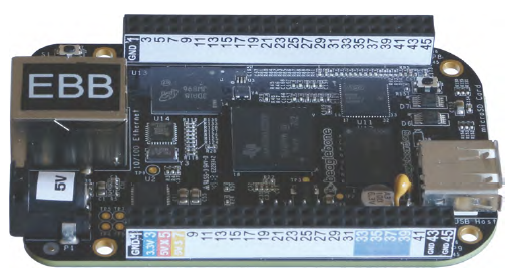
\includegraphics[width=0.82\textwidth]{eikona_19}
\caption[Η υπολογιστική πλατφόρμα BeagleBone Black]{Η υπολογιστική πλατφόρμα BeagleBone Black (έκδοση πλακέτας C με τυπωμένες ετικέτες των pins)\cite{46}}\label{eik19}
\end{figure}

Το BeagleBone Black κατασκευάζεται από την CircuitCo LLC στο Richardson του Τέξας προς όφελος της κοινότητας και των υποστηρικτών. Η CircuitCo παρέχει το RMA Support (εγγύηση επιστροφής) για το BeagleBone Black. O Jason Kridner της TexasInstruments χειρίζεται την προώθηση της κοινότητας και είναι ο εκπρόσωπος για την BeagleBoard.org. Το board σχεδιάστηκε από τον Gerald Coley, υπάλληλο της Texas Instruments και συνιδρυτή του BeagleBoard.org Foundation.

To PCB (Printed Circuit Board) έγινε από την CircuitCo και αυτή είναι η μόνη που χρηματοδοτεί την παραγωγή του προϊόντος. Το λογισμικό έχει γραφτεί και υποστηρίζεται από τους χιλιάδες υποστηρικτές-μέλη της κοινότητας, συμπεριλαμβανομένου του Jason Kridner, υπαλλήλους της Texas Instruments, Digi-Key και CircuitCo.

\section{Το υλικό (hardware) του BeagleBone Black}

Τα σχ.~\ref{eik20} και~\ref{eik21} δείχνουν λεπτομερώς τα κύρια συστήματα του BBB. Το πρώτο σετ των επεξηγήσεων, από 1 ως 8, ταυτοποιούν και περιγράφουν τα βασικά συστήματα πάνω στο BBB. Ο μικροεπεξεργαστής στο BBB είναι ένας Sitara AM335x Cortex A8 ARM από την Texas Instruments. Είναι ένας επεξεργαστής μειωμένου συνόλου οδηγιών υπολογισμού (RISC - Reduced Instruction Set Computing), έτσι στα 1000 MHz πραγματοποιεί 2000 εκατομμύρια εντολές ανά δευτερόλεπτο (MIPS - million instructions per second). Ο επεξεργαστής καταναλώνει περίπου 1~W όταν είναι σε αδράνεια (idle) και 2.3~W σε βαρύ φόρτο επεξεργασίας.

Το επόμενο σετ επεξηγήσεων, 9 ως 19, ταυτοποιεί διάφορους συνδέσμους πάνω στο BBB, τα φυσικά χαρακτηριστικά τους και τη λειτουργία τους.

\begin{enumerate}
\item {\large\textbf{Επεξεργαστής.}} AM335x:~ Ένας ισχυρός επεξεργαστής Sitara 1 GHz ARM-A8 της Texas Instruments που είναι ικανός για 2 δισεκατομμύρια εντολές ανά δευτερόλεπτο.
\item {\large\textbf{Γραφικά.}} HDMI Framer: Ο Framer μετατρέπει την LCD διεπαφή που είναι διαθέσιμη στον επεξεργαστή, σε ένα σήμα HDMI.
\item {\large\textbf{Μνήμη.}} 512 MB DDR3: Το ποσό της μνήμης του συστήματος επηρεάζει την απόδοση και τον τύπο των εφαρμογών που μπορούν να εκτελεστούν.
\item {\large\textbf{Αποθήκευση.}}~\phantom{k}eMMC (MMC1): Μια ενσωματωμένη on-board κάρτα πολυμέσων 2 GB(eMMC)--μια κάρτα SD σε τσιπ.
\item {\large\textbf{Διαχείριση ισχύος.}} TPS65217C: Ολοκληρωμένο κύκλωμα διαχείρισης ισχύος (PMIC). Ένα εξελιγμένο ολοκληρωμένο κύκλωμα διαχείρισης ισχύος που διαθέτει 4 LDO ρυθμιστές τάσης. Ελέγχεται μέσω I$^2$C.
\item {\large\textbf{Επεξεργαστής Ethernet.}} Ethernet PHY(10\slash100): Μπορεί να συνδεθεί απευθείας σε ένα δίκτυο (υποστηρίζει DHCP). Η φυσική διεπαφή LAN8710A συνδέει το φυσικό σύνδεσμο RJ45 με τον μικροεπεξεργαστή ARM.
\item {\large\textbf{LEDs.}} 7$\times$LEDs: LED παροχής(μπλε), 4 LEDs χρήστη (μπλε), και δύο LEDs στην υποδοχή RJ45 Ethernet (κίτρινο=σύνδεση 100M ενεργή, πράσινο=κίνηση).
\item {\large\textbf{Κουμπιά.}} 3 κουμπιά: Κουμπί εκκίνησης (on\slash off). Κουμπί επανεκκίνησης (reset) και διακόπτης επιλογής εκκίνησης για να διαλέξουμε αν θα εκκινήσει από την κάρτα SD ή από το eMMC.
\item {\large\textbf{Video out.}} micro-HDMI (HDMI-D): Για σύνδεση σε οθόνη.
\item {\large\textbf{Δίκτυο.}} Ethernet (RJ45): 10\slash100 Ethernet μέσω ενός συνδέσμου RJ45. Δεν υπάρχει on-board Wi-Fi.
\item {\large\textbf{DC παροχή.}} Παροχή 5~V DC (5.5mm): Για σύνδεση τροφοδοτικών 5~V στο BBB.
\item {\large\textbf{Κάρτα SD.}} Υποδοχή κάρτας (MMC0) (micro-SD): Μια υποδοχή κάρτας micro-SD 3.3~V. Το BBB μπορεί να εκκινήσει από αυτή την υποδοχή, μπορούμε να το φλασάρουμε μέσω αυτής ή μπορεί να χρησιμοποιηθεί για επιπλέον αποθηκευτικό χώρο όταν εκκινούμε από το eMMC.
\item {\large\textbf{Σειριακό Debug.}} Σύνδεσμος 6 pin (6$\times$0.1"):~(UART0) Χρησιμοποιείται με ένα σειριακό καλώδιο TTL3V3 για να συνδεθούμε στη σειριακή κονσόλα του BBB.\label{deb}
\item {\large\textbf{USB.}} 1$\times$USB 2.0 Client (mini-USB):~(USB0)Συνδέεται με τον υπολογιστή μας και μπορεί να τροφοδοτήσει απευθείας το BBB και\slash ή να επικοινωνήσει μαζί του.
\item {\large\textbf{USB.}} 1$\times$USB 2.0 Host (USB-A):~(USB1)Μπορούμε να συνδέσουμε USB περιφερειακά (π.χ. προσαρμογέα Wi-Fi, πληκτρολόγιο, κάμερα) στο BBB με αυτό το σύνδεσμο. Μπορούμε να χρησιμοποιήσουμε USB hub για να συνδέσουμε περισσότερες από μία συσκευή.
\itemrange{1} {\large\textbf{Headers επέκτασης P8 και P9.}} Δύο 2$\times$23 pin 0.1" θυληκοί headers: 92 pins σε δύο headers που πολυπλέκονται για να δώσουν πρόσβαση στα χαρακτηριστικά που περιγράφονται στον πίνακα~\ref{pinakas}. Δεν είναι όλες οι λειτουργίες διαθέσιμες ταυτόχρονα. Μπορούν να χρησιμοποιηθούν για να συνδέσουμε capes.
\item {\large\textbf{Άλλο Debug.}}~JTAG: Υπάρχει χώρος για ένα σύνδεσμο JTAG στη βάση του board.
\item {\large\textbf{Άλλη παροχή.}} Σύνδεσμοι μπαταρίας: Είναι δυνατό να συγκολλήσουμε pins και να τα χρησιμοποιήσουμε για να συνδέσουμε παροχή μπαταρίας.
\end{enumerate}

\begin{figure}[p]
\centering
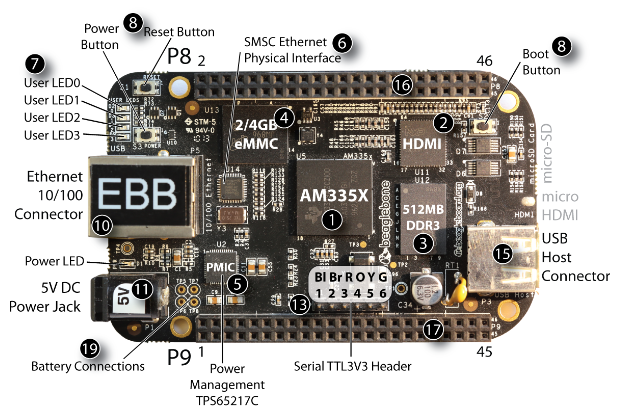
\includegraphics[width=\textwidth]{eikona_20}
\caption[Επάνω άποψη του BeagleBone Black]{Επάνω άποψη του BeagleBone Black\cite{46}}\label{eik20}
\end{figure}

\begin{figure}[p]
\centering
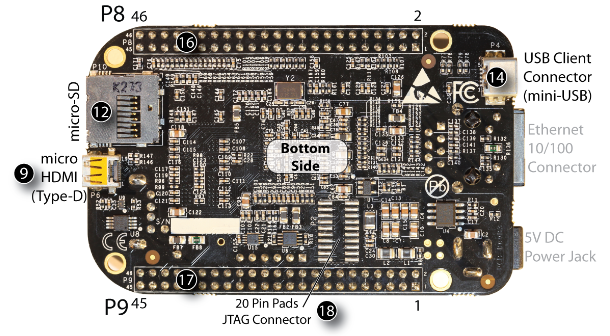
\includegraphics[width=\textwidth]{eikona_21}
\caption[Κάτω άποψη του BeagleBone Black]{Κάτω άποψη του BeagleBone Black\cite{46}}\label{eik21}
\end{figure}
\clearpage

Ο πίνακας~\ref{pinakas} περιγράφει τις διάφορες εισόδους και εξόδους που είναι διαθέσιμες στους headers P8 και P9. Υπάρχουν συνολικά 92 pins σε αυτούς τους headers (2$\times$46), όμως δεν είναι όλα διαθέσιμα για γενικού σκοπού εισόδους\slash εξόδους (\textenglish{general purpose input\slash outputs - GPIOs}). Πολλές από αυτές τις συνδέσεις έχουν μια προκαθορισμένη διαμόρφωση:
\begin{itemize}
\item[\textbf{--}] Οκτώ pins είναι συνδεδεμένα με ``ψηφιακή'' γη.
\item[\textbf{--}] Εννιά pins χρειάζονται για τις αναλογικές εισόδους (εφτά είσοδοι, γείωση και τάση αναφοράς 1.8~V).
\item[\textbf{--}] Έξι pins είναι κατανεμημένα σε παροχή τάσεων: 3.3V (έως 250mA) και 5V $V_{DD}$ (έως 1A εάν τροφοδοτείται από την DC υποδοχή -- η τροφοδοσία μπορεί να παρέχεται στο board μέσω των pins VDD\_5V.)
\item[\textbf{--}] Δύο είναι κατανεμημένα στους διαύλους I$^2$C.
\item[\textbf{--}] Δύο είναι κατανεμημένα στα κουμπιά εκκίνησης και επανεκκίνησης.
\end{itemize}

Οι υπόλοιποι 65 σύνδεσμοι είναι διαθέσιμοι να πολυπλεχθούν σε πολλές διαφορετικές λειτουργίες, μερικές εκ των οποίων αναφέρονται στον πίνακα~\ref{pinakas}.

\begin{table}
\centering
\footnotesize
{\renewcommand{\arraystretch}{1.5}
\renewcommand{\tabcolsep}{0.2cm}
\begin{tabular}{|C{1.5cm}|C{2cm}|L{10cm}|}
\hline
\textbf{GPIO} & 65$\times$GPIOs & Ο μέγιστος αριθμός των GPIOs είναι 65. Όλα τα GPIOs αντέχουν έως 3.3 V. Χρησιμοποιώντας τους διαύλους και τα interfaces που αναφέρονται παρακάτω, μειώνεται ο αριθμός των διαθέσιμων GPIOs.\\ \hline
\textbf{Αναλογική Έξοδος} & 8$\times$PWM & Έξοδοι διαμορφωμένες κατά PWM μας επιτρέπουν να στείλουμε ένα είδος μεταβλητής αναλογικής εξόδου (0 V έως 3.3 V). Το PWM μπορεί να χρησιμοποιηθεί για τον έλεγχο σερβοκινητήρων. Υπάρχουν οκτώ pins που μπορούν να δώσουν τέτοια έξοδο.\\ \hline
\textbf{Παροχή Τροφοδοσίας} & 5V, 3.3V, 1.8V & Παροχές των 5 και 3.3 V και μια παροχή αναφοράς 1.8 V για τις αναλογικές εισόδους. Οκτώ pins στους headers οδηγούν στην ``κανονική'' γη.\\ \hline
\textbf{Χρονιστές} & 4$\times$Χρονιστές & Μπορούν να χρησιμοποιηθούν για να κατασκευάσουν εξωτερικά ρολόγια για τη διασύνδεση με συσκευές.\\ \hline
\textbf{Δίαυλοι} & 2$\times$I$^2$C & Το I$^2$C είναι ένας ψηφιακός δίαυλος που μας επιτρέπει να συνδέσουμε διάφορες μονάδες (modules) σε καθέναν από αυτούς τους διαύλους των δύο καλωδίων ταυτόχρονα.\\ \cline{2-3}
 & 4$\times$UART & Χρησιμοποιούνται για σειριακή επικοινωνία μεταξύ δύο συσκευών. Το UART0 είναι ο σύνδεσμος για το σειριακό Debug που περιγράφεται στο \ref{deb}(σελ.~\pageref{deb}).\\ \cline{2-3}
 & 2$\times$CAN & Ο δίαυλος CAN χρησιμοποιείται για δίκτυα περιοχής ελεγκτών (Controller Area Networks), συνήθως σε βιομηχανικές διαδικασίες ή οχήματα για να επικοινωνούν μέσω διαφόρων δικτυωμένων συστημάτων.\\ \cline{2-3}
 & 2$\times$SPI & Η σειριακή περιφεριακή διεπαφή (Serial Peripheral Interface) παρέχει μια σύγχρονη σύνδεση σειριακών δεδομένων για μικρές αποστάσεις. Χρησιμοποιεί μια διαμόρφωση αφέντη\slash σκλάβου και απαιτεί τέσσερα καλώδια για την επικοινωνία με το BBB.\\ \cline{2-3}
 & GPMC & Ο ελεγκτής μνήμης γενικού σκοπού (General Purpose Memory Controller) χρησιμοποιείται για να συνδεόμαστε σε εξωτερικές συσκευές μνήμης όπως FPGAs ή ASICs.\\ \cline{2-3}
 & 2$\times$MMC & Δίαυλοι διεπαφής που χρησιμοποιούνται για να συνδέσουμε την κάρτα micro-SD και το eMMC στον επεξεργαστή.\\ \cline{2-3}
 & LCD & Χρήσιμος για οθόνες LCD (π.χ. για LCD capes). Αυτή η διεπαφή συγκρούεται με τον HDMI Framer (μόνο ένα από τα δύο μπορεί να χρησιμοποιηθεί ταυτόχρονα).\\ \cline{2-3}
 & 2$\times$McASP & Σειρακή θύρα ήχου γενικού σκοπού -- πολυκαναλική σειριακή θύρα ήχου (McASP), συνδεδεμένη στον HDMI Framer.\\
\hline
\end{tabular}
}
\caption{Διαθέσιμη λειτουργικότητα στους headers P8 και P9}\label{pinakas}
\end{table}
\clearpage

\begin{figure}
\centering
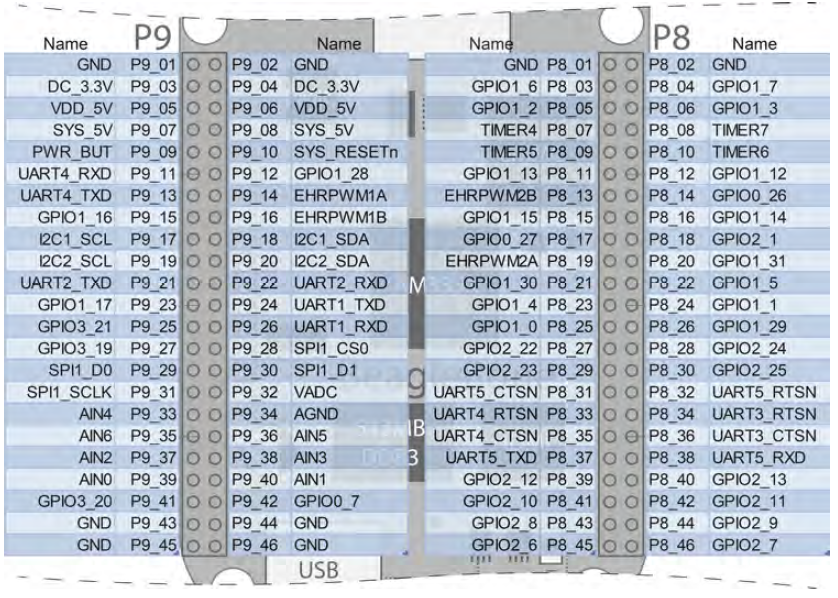
\includegraphics[width=0.95\textwidth]{eikona_22}
\caption[Οι headers P8\slash P9 του BBB]{Οι headers P8\slash P9 του BBB με ονόματα στα pins, που περιγράφουν την προκαθορισμένη λειτουργικότητά τους\cite{46}}\label{eik22}
\end{figure}

\section{Η αρχιτεκτονική ARM}

Η ARM είναι μια αρχιτεκτονική συνόλου οδηγιών για επεξεργαστές υπολογιστών βασισμένη στην αρχιτεκτονική μειωμένου συνόλου οδηγιών υπολογιστών (RISC) που αναπτύχθηκε από την Βρετανική εταιρεία ARM Holdings. Μια προσέγγιση σχεδιασμού υπολογιστών βασισμένη στην RISC σημαίνει ότι οι επεξεργαστές ARM απαιτούν εξαιρετικά λιγότερα τρανζίστορ από ότι οι τυπικοί επεξεργαστές CISC x86 που χρησιμοποιούνται στους περισσότερους προσωπικούς υπολογιστές.

Αυτή η προσέγγιση μειώνει το κόστος και τη χρήση ενέργειας. Τέτοιες μειώσεις είναι επιθυμητά χαρακτηριστικά για τις ελαφρές, φορητές, -που λειτουργούν με μπαταρία- συσκευές, συμπεριλαμβανομένων των έξυπνων τηλεφώνων, φορητών υπολογιστών, tablet και notepad υπολογιστών, καθώς και άλλων ενσωματωμένων συστημάτων.

Η εταιρεία ARM Holdings αναπτύσσει το σύνολο οδηγιών και αρχιτεκτονικής για προϊόντα βασισμένα στην ARM αλλά δεν κατασκευάζει προϊόντα.

Η εταιρεία κατά καιρούς εκδίδει ενημερώσεις για τους πυρήνες της. Οι τρέχοντες πυρήνες από την ARM Holdings υποστηρίζουν ένα χώρο διεύθυνσης 32-bit και αριθμητική 32-bit. Η αρχιτεκτονική ARM v8-A, που ανακοινώθηκε τον Οκτώβριο 2011, προσθέτει στήριξη για 64- bit χώρο διεύθυνσης και αριθμητική 64-bit. Οι οδηγίες για τους πυρήνες ARM Holdings έχουν οδηγίες 32 bits εύρους, σταθερού μήκους, αλλά οι μετέπειτα εκδόσεις της αρχιτεκτονικής υποστηρίζουν επίσης ένα σύνολο οδηγιών μεταβλητού μήκους που προσφέρει οδηγίες τόσο 32 όσο και 16 bits εύρους για βελτιωμένη πυκνότητα πυρήνα. Μερικοί πυρήνες μπορούν επίσης να προσφέρουν εκτέλεση υλικού των Java byte codes.

H ARM Holdings δίνει την άδεια χρήσης των σχεδίων chip και των ARM αρχιτεκτονικών συνόλων οδηγιών σε τρίτα μέρη, οι οποίοι σχεδιάζουν τα δικά τους προϊόντα που εφαρμόζουν μια από αυτές τις αρχιτεκτονικές συμπεριλαμβανομένων συστημάτων-on-chip(SoC), που ενσωματώνουν μνήμη, interfaces, ραδιόφωνα, κ.α. Οι εταιρείες που φτιάχνουν chips τα οποία εφαρμόζουν την ARM αρχιτεκτονική περιλαμβάνουν τις: Apple, Applied Micro, Atmel, Broadcom, Freescale Semiconductor, Nvidia, NXP, Qualcomm, Samsung Electronics, ST Microelectronics και Texas Instruments.

Παγκοσμίως, η ARM είναι η πιο ευρέως χρησιμοποιούμενη αρχιτεκτονική συνόλου οδηγιών όσον αφορά την παραγόμενη ποσότητα. Η χαμηλή κατανάλωση ενέργειας των επεξεργαστών ARM τους έχει κάνει πολύ δημοφιλείς: πάνω από 50 δισεκατομμύρια ARM επεξεργαστές έχουν παραχθεί μέχρι το 2014, εκ των οποίων τα 10 δις μέσα στο 2013 και τα chips που βασίζονται στην ARM βρίσκονται σχεδόν στο 60\%{} των κινητών συσκευών στον κόσμο.

\section{UART}

Ένας καθολικός ασύγχρονος παραλήπτης\slash εκπομπός (\textenglish{universal asynchronous receiver\slash transmitter - UART}) είναι μια περιφερειακή συσκευή μικροεπεξεργαστή που χρησιμοποιείται για τη σειριακή μεταφορά δεδομένων, ένα bit τη φορά, μεταξύ δύο ηλεκτρονικών συσκευών. Αρχικά τα UART ήταν αυτόνομα ολοκληρωμένα κυκλώματα (IC), αλλά τώρα είναι συχνά ενσωματωμένα στον μικροεπεξεργαστή\slash μικροελεγκτή. Ένα UART δεν είναι, αυστηρά μιλώντας, ένας δίαυλος, αλλά η ικανότητά του να πραγματοποιεί επικοινωνίες σειριακών δεδομένων συμπίπτει με τις παρόμοιες ικανότητες των διαύλων I$^2$C και SPI. Το UART περιγράφεται ως ασύγχρονο γιατί ο αποστολέας δεν χρειάζεται να στείλει ένα σήμα ρολογιού στον παραλήπτη για να συγχρονίσει τη μετάδοση, αλλά έχει συμφωνηθεί μια δομή επικοινωνίας που χρησιμοποιεί bits εκκίνησης και τερματισμού για να συγχρονίζει τη μετάδοση δεδομένων. Επειδή δεν απαιτείται ρολόι, τα δεδομένα συνήθως στέλνονται χρησιμοποιώντας μόνο δύο γραμμές σήματος. Όπως σε μια συνηθισμένη γραμμή τηλεφώνου, η σύνδεση αποστολής δεδομένων (\textenglish{transmit data connection - TXD}) από το ένα άκρο συνδέεται στη σύνδεση λήψης δεδομένων (\textenglish{receive data connection - RXD}) στο άλλο άκρο της σύνδεσης, και το αντίστροφο.

Παραδοσιακά, τα UART χρησιμοποιούνταν με μετατροπείς επιπέδου\slash οδηγούς γραμμής για να πραγματοποιήσουν διεπαφές όπως RS-232 ή rs-485, αλλά για επικοινωνίες μικρής απόστασης, είναι δυνατό να χρησιμοποιθεί το αρχικό λογικό επίπεδο για τις εξόδους και εισόδους του UART για να δοθεί η δυνατότητα σε δύο UART να επικοινωνήσουν μεταξύ τους.

Ο αριθμός των συμβόλων ανά δευτερόλεπτο είναι γνωστός ως baud rate ή ρυθμός διαμόρφωσης. Με συγκεκριμένες μεθόδους διαμόρφωσης ένα σύμβολο μπορεί να χρησιμοποιηθεί για να αναπαριστά δύο bits (π.χ. τέσσερις καταστάσεις, αν χρησιμοποιηθεί QPSK). Έτσι, το bit rate θα ήταν διπλάσιο του baud rate. Ωστόσο, για μια απλή σύνδεση δύο επιπέδων, το baud rate είναι το ίδιο με το bit rate.

Ο εκπομπός και ο παραλήπτης συμφωνούν για το bit rate προτού ξεκινήσει η επικοινωνία. Το byte rate είναι κατάτι μικρότερο από το $1/8$ του bit rate, καθώς υπάρχουν επικεφαλής bits που σχετίζονται με τη σειριακή μετάδοση δεδομένων. Η μετάδοση ξεκινά όταν ο εκπομπός στείλει ένα bit εκκίνησης (λογικό μηδέν), όπως δείχνεται στο σχ.~\ref{eik23}. Στο άκρο του παραλήπτη, ανιχνεύεται η πίπτουσα παρυφή του bit εκκίνησης και μετά από μιάμιση περίοδο bit, δειγματοληπτείται η τιμή του πρώτου bit. Κάθε ακόλουθο bit δειγματοληπτείται μετά από περιόδους ενός bit, μέχρι να μεταφερθεί ο συμφωνηθείς αριθμός από bits (συνήθως 7 ή 8). Το bit ισοτιμίας είναι προαιρετικό (αν και πρέπει και οι δύο συσκευές να είναι ρυθμισμένες ώστε να το χρησιμοποιύν ή όχι) και αν χρησιμοποιηθεί, μπορεί να αναγνωρίσει εάν έχει συμβεί κάποιο λάθος κατά τη μετάδοση. Θα είναι λογικό ένα ή μηδέν, ανάλογα με το είδος της ισοτιμίας που έχει συμφωνηθεί (άρτια ή περιττή). Στο τέλος, ένα bit τερματισμού στέλνεται (ή προαιρετικά δύο bits τερματισμού), που η τιμή του είναι πάντα λογικό ένα.

\begin{figure}
\centering
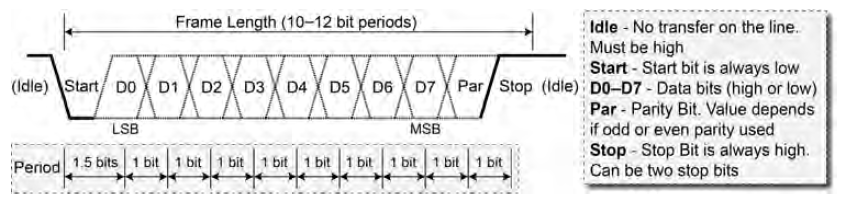
\includegraphics[width=\textwidth]{eikona_23}
\caption[Πρότυπο μετάδοσης UART για τη μεταφορά ενός byte]{Πρότυπο μετάδοσης UART για τη μεταφορά ενός byte\cite{46}}\label{eik23}
\end{figure}

\paragraph{UARTs πάνω στο BBB}

Το BeagleBone Black έχει πάνω του τέσσερα UART που είναι προσβάσιμα μέσω των headers P8 και P9, στις τοποθεσίες των υποδοχών που αναγράφονται στον πίνακα~\ref{pinakas2}

\begin{table}
\centering
\caption[Τοποθεσίες στους headers για πρόσβαση στα UART]{Τοποθεσίες των pins στους headers του BBB για πρόσβαση στα UART (κατάσταση πολυπλεξίας σε παρένθεση)}\label{pinakas2}
\vspace*{1em}
\footnotesize
{\renewcommand{\arraystretch}{1.5}
\renewcommand{\tabcolsep}{0.2cm}
\begin{tabular}{|C{2cm} L{2cm} L{2cm} L{2.5cm} L{2cm} L{2cm}|}
\hline
 & \textbf{UART1} & \textbf{UART2} & \textbf{UART3} & \textbf{UART4} & \textbf{UART5}\\ \hline
TXD & P9\_24(0) & P9\_21(1) & Δεν εκτίθεται & P9\_13(6) & P8\_37(4)\\ \hline
RXD & P9\_26(0) & P9\_22(1) & Δεν εκτίθεται & P9\_11(6) & P8\_38(4)\\
\hline
\end{tabular}
}
\end{table}
\clearpage

\section{Αντίστοιχες πλατφόρμες με το BeagleBone Black}

Καθώς υπάρχουν και άλλες πλατφόρμες παρόμοιες με το BeagleBone διαθέσιμες στην αγορά, θεωρήσαμε σκόπιμο να κάνουμε μια συνοπτική παρουσίαση των χαρακτηριστικών τους, και επίσης να γίνει και μια σύγκριση μεταξύ των δημοφιλέστερων από αυτές με το Beaglebone, σε αυτήν την υποενότητα. Θα αναλύσουμε τα πλεονεκτήματα και τα μειονεκτήματα της κάθε πλατφόρμας και θα παρουσιάσουμε τους λόγους που μας οδήγησαν τελικά στην επιλογή χρήσης του BeagleBone έναντι των άλλων.

\subsection{Χαρακτηριστικά πλατφόρμας}

\subsubsection{Arduino}

Το Arduino είναι μια open source πλατφόρμα η οποία έχει ενσωματωμένο ένα μικροελεγκτή. Η πλατφόρμα αυτή έχει εισόδους και εξόδους τις οποίες μπορούμε να προγραμματίσουμε μέσω ενός φιλικού περιβάλλοντος το οποίο διατίθεται δωρεάν. Κατασκευάστηκε για εκπαιδευτικούς λόγους από τους Massimo Banzi και David Cuartielles.

Η γλώσσα προγραμματισμού που χρησιμοποιεί είναι η Wiring, η οποία ουσιαστικά πρόκειται για τη C++ με κάποιες μικρές αλλαγές. Έχει την δυνατότητα να χρησιμοποιηθεί για την ανάπτυξη ανεξάρτητων διαδραστικών αντικειμένων, αλλά και να συνδεθεί με υπολογιστή μέσω προγραμμάτων σε Processing, Max\slash MSP, PureData, SuperCollider.

Το σχέδιο του Arduino είναι ελεύθερο και δωρεάν και έτσι μπορεί να κατασκευασθεί από τον καθένα. Για αυτόν τον λόγο έχουν δημιουργηθεί και διάφορες εκδόσεις, μερικές από τις οποίες είναι οι εξής: Decimila, Due, Duemilanove, Uno, Leonardo, Mega, Mega 2560, Fio, Nano.

Οι εφαρμογές που μπορεί να χρησιμοποιηθεί το Arduino είναι πάρα πολλές λόγω και των διαφόρων shields (Περιφερειακές συσκευές) που μπορούν να συνδεθούν, όπως αισθητήρες, συνδέσεις με άλλες ηλεκτρονικές συσκευές μέσω των αντίστοιχων shields (wireless, Ethernet, usb) καθώς και πολλά ακόμα περιφερειακά.
\clearpage
\begin{figure}[!htb]
\centering
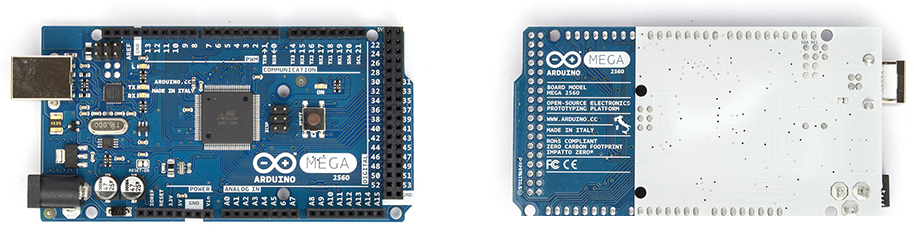
\includegraphics[width=\textwidth]{img_arduino}
\caption[Μπροστινή και πίσω άποψη του Arduino Mega 2560]{Μπροστινή και πίσω άποψη του Arduino Mega 2560\cite{arduino}}
\end{figure}

Τα τεχνικά χαρακτηριστικά του Arduino είναι τα εξής:

\begin{table}[!hb]
\centering
{\renewcommand{\arraystretch}{1.5}
\renewcommand{\tabcolsep}{0.2cm}
\footnotesize
\begin{tabular}{L{0.4\textwidth} L{0.6\textwidth}}
\hline
\textbf{Μικροελεγκτής:} & ATmega2560\\ \hline
\textbf{Τάση λειτουργίας:} & 5~V\\ \hline
\textbf{Τάση εισόδου(προτεινόμενη):} & 7-12~V\\ \hline
\textbf{Τάση εισόδου(όρια):} & 6-20~V\\ \hline
\textbf{Ψηφιακές Είσοδοι\slash Έξοδοι:} & 54 pins(εκ των οποίων οι 15 παρέχουν PWM έξοδο)\\ \hline
\textbf{Αναλογικές Είσοδοι:} & 16 pins\\ \hline
\textbf{Συνεχές ρεύμα ανά I\slash O pin:} & 40~mA\\ \hline
\textbf{Συνεχές ρεύμα για το pin 3.3~V:} & 50~mA\\ \hline
\textbf{Μνήμη Flash:} & 256~KB από τα οποία τα 8 χρησιμοποιούνται από τον bootloader\\ \hline
\textbf{SRAM:} & 8~KB\\ \hline
\textbf{EEPROM:} & 4~KB\\ \hline
\textbf{Συχνότητα ρολογιού:} & 16~MHz\\ \hline
\end{tabular}
}
\end{table}
%\clearpage

\subsubsection{Raspberry Pi~(Model B)}

Το Raspberry Pi είναι μια πλακέτα μεγέθους πιστωτικής κάρτας που συνδέεται στην τηλεόραση και σε ένα πληκτρολόγιο. Είναι μια μικρογραφία ενός ARM-based υπολογιστή που μπορεί να χρησιμοποιηθεί για πολλές από τις εργασίες που χρησιμοιποιείται και ένας κανονικός υπολογιστής, όπως τα λογιστικά φύλλα, επεξεργασία κειμένου και παιχνίδια. Έχει τη δυνατότητα να αναπαράγει βίντεο υψηλής ανάλυσης (HD).
\clearpage
\begin{figure}[!htb]
\centering
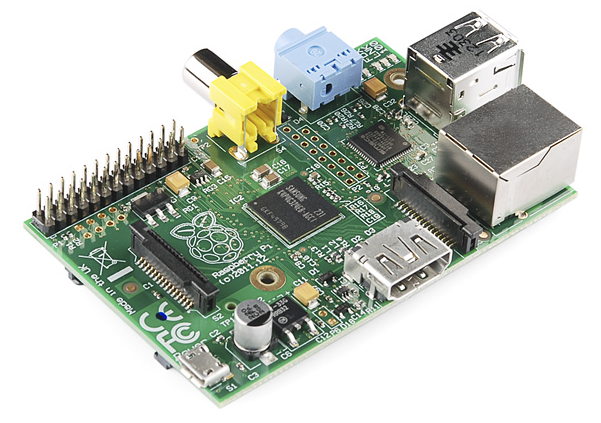
\includegraphics[scale=0.6]{img_rasp}
\caption[Το Raspberry Pi Model B]{Το Raspberry Pi Model B\cite{raspberry}}
\end{figure}

Το Raspberry Pi Model B 512MB RAM έχει τα ακόλουθα τεχνικά χαρακτηριστικά:
\begin{table}[!hb]
\centering
{\renewcommand{\arraystretch}{1.5}
\renewcommand{\tabcolsep}{0.2cm}
\footnotesize
\begin{tabular}{L{0.3\textwidth} L{0.65\textwidth}}
\hline
\textbf{SoC:} & Broadcom BCM2835\\ \hline
\textbf{Επεξεργαστής:} &  ARM1176JZF-S στα 700~MHz\\ \hline
\textbf{GPU:} & Broadcom VideoCore IV. Η GPU παρέχει OpenGLES 2.0 και 1080p30 H.264 high-profile αποκωδικοποίηση.\\ \hline
\textbf{RAM:} & 512~MB\\ \hline
\textbf{Συνδεσιμότητα:} & 2$\times$USB 2.0 Θύρες\\ \hline
\textbf{Έξοδος βίντεο:} & Σύνθετο (PAL και NTSC), HDMI ή Raw LCD(DSI)\\ \hline
\textbf{Έξοδος ήχου:} & Μέσω υποδοχής 3.5~mm ή ήχος μέσω HDMI\\ \hline
\textbf{Αποθήκευση:} & SD\slash MMC\slash SDIO\\ \hline
\textbf{Δίκτυο:} & 10\slash 100 Ethernet (RJ 45)\\ \hline
\textbf{Περιφερειακά χαμηλού επιπέδου:} & \begin{itemize} 
\item 8$\times$GPIO
\item UART
\item δίαυλος I$^2$C
\item δίαυλος SPI με δύο chip select
\item +3.3 V, +5 V και γείωση
\end{itemize}\\ \hline
\end{tabular}
}
\end{table}
\clearpage
\subsubsection{Bif\mbox{}ferboard}

To Bif\mbox{}ferboard είναι μια πλατφόρμα η οποία <<τρέχει>> Linux, καταναλώνει μόλις 1~W και χάρη στη μικρή κατανάλωση ισχύος μπορεί να τροφοδοτηθεί μέσω USB. Έχει όλες τις απαραίτητες συνδέσεις τις οποίες μπορεί να χρειαστούμε σε ένα τέτοιο σύστημα.

Παρακάτω παραθέτουμε τα τεχνικά χαρακτηρικά:
\begin{table}[!hb]
\centering
{\renewcommand{\arraystretch}{1.5}
\renewcommand{\tabcolsep}{0.2cm}
\footnotesize
\begin{tabular}{L{0.3\textwidth} L{0.65\textwidth}}
\hline
\textbf{Επεξεργαστής:} & 150MHz RDC, συμβατός με Intel 486SX\\ \hline
\textbf{Κατανάλωση:} & 1 Watt (200~mA στα 5~V)\\ \hline
\textbf{Διαστάσεις:} & 68mm$\times$28mm$\times$19mm\\ \hline
\textbf{Μνήμη:} & 32~MB SDRAM\slash 1~MB Flash\\ \hline
\textbf{Συνδεσιμότητα:} & OHCI\slash EHCI USB 2.0\\ \hline
\textbf{Δίκτυο:} & 10\slash 100 Ethernet\\ \hline
\textbf{Debug:} & 4-pin JTAG (μπορεί να χρησιμοποιηθεί και σαν GPIO)\\ \hline
\textbf{Είσοδος\slash Έξοδος:} & 2 GPIO (1 LED, 1 κουμπί)\\ \hline
\textbf{Λειτουργικό Σύστημα:} & Linux 2.6.27.5 και OpenWrt\\ \hline
\end{tabular}
}
\end{table}

\begin{figure}[!hbt]
\centering
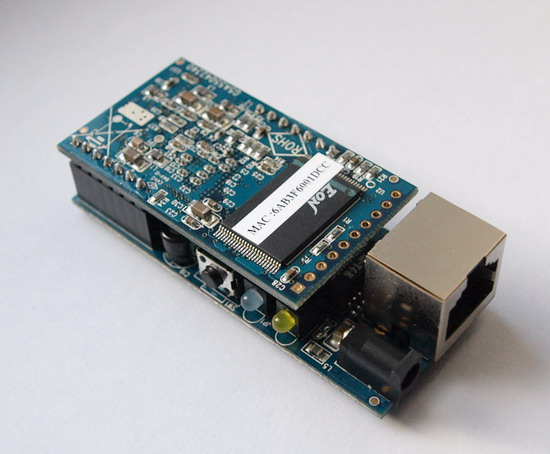
\includegraphics[width=0.75\textwidth]{img_bifferboard2}
\caption[Το Bif\mbox{}ferboard]{Το Bif\mbox{}ferboard\cite{bifferboard}}
\end{figure}
%\clearpage

Το Bif\mbox{}ferboard έχει δυο μέρη από τα οποία αποτελείται: την πλακέτα του επεξεργαστή και την πλακέτα των συσκευών εισόδου\slash εξόδου όπου παρέχεται δυνατότητα δικτύωσης μέσω Ethernet και σύνδεσης usb.
\begin{figure}[!h]
\centering
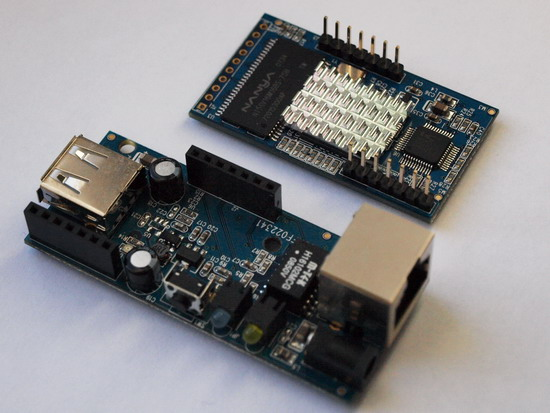
\includegraphics[width=0.85\textwidth]{img_bifferboard}
\caption[Τα δύο μέρη του Bif\mbox{}ferboard]{Τα δύο μέρη του Bif\mbox{}ferboard\cite{bifferboard}}
\end{figure}

\subsubsection{Parallela}

Η πλατφόρμα Parallella είναι ένας μικρός υπολογιστής σε μέγεθος πιστωτικής κάρτας, ο οποίος βασίζεται στα τσιπ πολλαπλών πυρήνων Epiphany, που αναπτύχθηκαν από την Adapteva. Αυτή η προσιτή πλατφόρμα έχει σχεδιαστεί για την ανάπτυξη και πραγματοποίηση εφαρμογών υψηλής απόδοσης, παράλληλης επεξεργασίας που έχουν αναπτυχθεί για να επωφεληθούν από το ενσωματωμένο τσιπ Epiphany. Τα τσιπ Epiphany 16 ή 64 πυρήνων αποτελούνται από μια κλιμακούμενη διάταξη από απλούς RISC επεξεργαστές προγραμματιζόμενους σε C\slash C++, συνδεδεμένους μεταξύ τους με ένα γρήγορο on chip δίκτυο μέσα σε μια αρχιτεκτονική μιας μοναδικής κοινόχρηστης μνήμης.

Τα χαρακτηριστικά της Parallela είναι τα παρακάτω:
\begin{table}[t]
\centering
{\renewcommand{\arraystretch}{1.5}
\renewcommand{\tabcolsep}{0.2cm}
\footnotesize
\begin{tabular}{L{0.3\textwidth} L{0.65\textwidth}}
\hline
\textbf{Επεξεργαστής:} & Zynq-7000 Series Dual-core ARM A9 (Z-7010 ή Z-7020)\\ \hline
\textbf{Onboard Chip:} & 16 ή 64-πύρηνος επιταχυντής πολλαπλών πυρήνων Epiphany\\ \hline
\textbf{Μνήμη:} & 1 GB RAM\\ \hline
\textbf{Αποθήκευση:} & Κάρτα MicroSD\\ \hline
\textbf{Συνδεσιμότητα:} & 2$\times$USB 2.0\\ \hline
\textbf{Είσοδος\slash Έξοδος:} & 4 συνδέσεις επέκτασης γενικού σκοπού\\ \hline
\textbf{Δίκτυο:} & 10\slash 100\slash 1000 Ethernet\\ \hline
\textbf{Έξοδος βίντεο:} & Θύρα HDMI\\ \hline
\textbf{Λειτουργικό σύστημα:} & Linux\\ \hline
\end{tabular}
}
\end{table}

\begin{figure}[!hb]
\centering
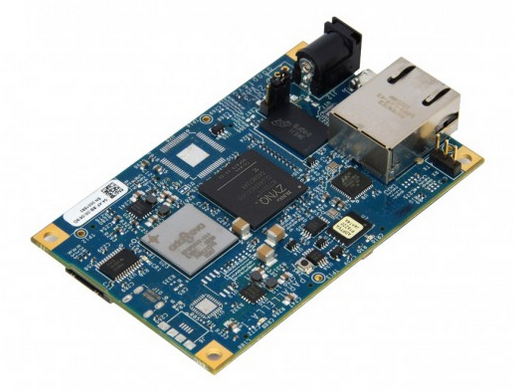
\includegraphics[width=0.85\textwidth]{img_parallela}
\caption[Η πλατφόρμα Parallela]{Η πλατφόρμα Parallela\cite{parallela}}
\end{figure}
\clearpage

\subsection{Σύγκριση πλατφορμών}

Παρακάτω πρόκειται να αναλύσουμε τις διαφορές, τα πλεονεκτήματα και τα μειονεκτήματα από τις τρεις πιο δημοφιλείς πλατφόρμες προγραμματισμού που αναφέραμε προηγουμένως, καθώς και να εξηγήσουμε τους λόγους που συνέβαλαν ώστε να επιλέξουμε το BeagleBone Black ως την πλατφόρμα προγραμματισμού στην οποία στηρίχθηκε και υλοποιήθηκε η συγκεκριμένη διπλωματική εργασία.

\begin{table}[!hp]
\centering
{\renewcommand{\arraystretch}{1.5}
\renewcommand{\tabcolsep}{0.2cm}
\footnotesize
\begin{tabular}{L{0.25\textwidth} R{0.2\textwidth} R{0.2\textwidth} R{0.25\textwidth}}
\hline
 & \textbf{Arduino} & \textbf{Raspberry Pi} & \textbf{BeagleBone Black}\\ \hline
\textbf{Επεξεργαστής} & ATmega2560 & ARM 11 & ARM Cortex A-8\\ \hline
\textbf{Συχνότητα} & 16 MHz & 700 MHz & 1 GHz\\ \hline
\textbf{RAM} & 256 KB & 512 MB & 512 MB\\ \hline
\textbf{USB} & 1 & 2 & 1\\ \hline
\textbf{Audio} & N\slash A & HDMI, Analog & MiniHDMI\\ \hline
\textbf{Video} & N\slash A & HDMI, Analog & MiniHDMI\\ \hline
\textbf{Ethernet} & N\slash A & 10\slash 100 & 10\slash 100\\ \hline
\textbf{I\slash O} & 54 Digital, 14 Analog & 8 GPIO & GPIO, GPMC, MMC1, AIN, Serial Ports, CAN0\\ \hline
\textbf{Μέγεθος} & 108$\times$53$\times$15 mm & 85.6$\times$53.98$\times$17 mm & 88.98$\times$54.63$\times$18.84 mm\\ \hline
\textbf{Λειτουργικό Σύστημα} & Linux, Windows & Linux & Android, Linux, Windows κ.ά.\\ \hline
\textbf{Προγραμματιστικό Περιβάλλον} & Arduino IDE & Linux, IDLE, OpenEmbedded, QEMU, Scratchbox, Eclipse & Python, Scratch, Linux, Eclipse, Android SDK, Cloud9, Bonescript\\ \hline
\textbf{Κόστος} & 47.5~\euro & 41~\euro & 55~\euro\\ \hline
\end{tabular}
}
\caption{Σύγκριση Arduino, Raspberry Pi και BeagleBone Black}
\end{table}
\clearpage

\subsubsection{Arduino}

To Arduino είναι βασικό για την κοινότητα του <<Κάν'το-μόνος-σου>> επειδή είναι ανοιχτό, εύκολο στην ανάπτυξη εφαρμογών, καταναλώνει ελάχιστη ενέργεια και είναι εύκολο στη συναρμολόγηση. Επίσης, είναι σχεδιασμένο ειδικά για αρχάριους, οπότε όλοι μπορούν να ``παίξουν'' και να το συνδέσουν με εξωτερικές συσκευές. Βασικά το Αrduino είναι ένα μικρό motherboard το οποίο δέχεται και αποθηκεύει κώδικες από τον υπολογιστή. Μπορεί να κάνει απλά αλλά ενδιαφέροντα πράγματα, όπως να ελέγχει το φωτισμό ή να προγραμματίζει ποτιστικά και άλλα πολλά.

\paragraph{Πλεονεκτήματα:} Εκτός του απλού Arduino, υπάρχουν πολλές παραλλαγές του για να επιλέξει κανείς. Επίσης το Arduino καταναλώνει ελάχιστη ενέργεια, οπότε είναι ιδανικό για project που χρειάζονται πολύ χρόνο ή που χρησιμοποιούν μπαταρίες. Το πιο σημαντικό είναι ότι το Arduino είναι εξαιρετικά δημοφιλές, οπότε μπορεί κανείς εύκολα να βρει υποστήριξη και υλικό. Τέλος, το Arduino μπορεί να συνδεθεί σχεδόν με τα πάντα.

\paragraph{Μειονεκτήματα:} Το Arduino είναι για αρχάριους αλλά χρειάζεται κάποιος χρόνος για να συνηθίσει ο χρήστης κάτι που δεν έχει γραφικό περιβάλλον. Επίσης, δεν μπορεί να διαχειριστεί πολλές διαφορετικές διεργασίες ταυτόχρονα, οπότε δεν είναι κατάλληλο για project που χρειάζονται μεγάλη υπολογιστική ισχύ.

\paragraph{Σε τι εργασίες είναι χρήσιμο:} Το Arduino είναι καλύτερο για εργασίες που αφορούν ένα και μόνο αντικείμενο, για παράδειγμα, ένα σύστημα στο οποίο το στεγνωτήριο μας στέλνει μήνυμα όταν είναι έτοιμα τα ρούχα ή ένα θυροτηλέφωνο. Επίσης είναι καλό στο να χειρίζεται αντικείμενα, δηλαδή είναι κατάλληλο αν θέλει κάποιος να χρησιμοποιήσει τα στόρια του παραθύρου ή μια κλειδαριά. Οπότε, αν σχεδιάζουμε κάτι απλό, όπως έναν πίνακα ελέγχου για τον κήπο, το Arduino είναι ιδανικό. Αν όμως θέλουμε να συνδέσουμε αυτόν τον πίνακα με το Internet και να έχουμε πλήρη αυτοματισμό, τότε πιθανότατα θα συναντήσουμε δυσκολίες.

\subsubsection{Raspberry Pi Model B}

Το Raspberry Pi είναι ένας μικροϋπολογιστής ο οποίος τρέχει Linux μέσω κάρτας SD και μπορεί να εκτελέσει πολλές διαφορετικές εντολές. Στην ουσία, είναι ένας μικρός υπολογιστής με Linux ο οποίος μπορεί να κάνει ό,τι και ένας μεγάλος, με μόνο 35\$. Διαθέτει 2 θύρες USB και μία HDMI, οπότε μπορούμε να το χρησιμοποιήσουμε για οποιαδήποτε εργασία απαιτεί Linux. Σε γενικές γραμμές, το Raspberry είναι καλό όταν χρειαζόμαστε απεικόνιση ή σύνδεση στο Διαδίκτυο.

\paragraph{Πλεονεκτήματα:} Η θύρα HDMI του δίνει τη δυνατότητα να συνδεθεί με τηλεόραση και στις δυο USB μπορούμε να συνδέσουμε πληκτρολόγιο και ποντίκι πολύ εύκολα. Επίσης, μέσω της θύρας Ethernet μπορούμε να συνδεθούμε στο διαδίκτυο. Τέλος, επειδή το λειτουργικό τρέχει μέσω SD κάρτας, μπορούμε να τρέξουμε διαφορετικά λειτουργικά συστήματα αλλάζοντας απλά την κάρτα.

\paragraph{Μειονεκτήματα:} Αν και είναι καλό για κάθε εργασία στην οποία θα χρησιμοποιούσαμε υπολογιστή, δεν έχει τόσες δυνατότητες στη σύνδεση με εξωτερικούς αισθητήρες ή διακόπτες (όπως το Arduino ή το BeagleBone). Οπότε αν θέλουμε να συνδεθούμε με τις ηλεκτρικές συσκευές του σπιτιού ή με τον φωτισμό, το Raspberry δεν είναι πολύ καλή επιλογή.

\paragraph{Σε τι εργασίες είναι χρήσιμο:} Είναι χρήσιμο για εργασίες στις οποίες απαιτείται γραφικό περιβάλλον ή σύνδεση με το διαδίκτυο. Είναι καλό για αρχάριους ως εκπαιδευτικό project, προτιμάται όμως και ως Media Center και all-in-one retro game center.

\subsubsection{BeagleBone Black}

To BeagleBone Black είναι ένας συνδυασμός Arduino και Raspberry Pi. Έχει την ισχύ του Raspberry και τις επιλογές για εξωτερική σύνδεση που έχει το Arduino. Επειδή δε χρειάζεται απεικόνιση όπως το Raspberry Pi για να ξεκινήσει, το BeagleBoard αφορά περισσότερο προχωρημένους χρήστες και προγραμματιστές. Έχει και αυτό Linux, οπότε μπορεί να χρησιμοποιηθεί ως υπολογιστής από μόνο του. Επίσης, μπορούμε να εγκαταστήσουμε πολλά διαφορετικά λειτουργικά, όπως το Android, Windows Embedded. Είναι πιο δύσκολο στο χειρισμό από το Raspberry, αλλά μπορούμε να κάνουμε περισσότερα πράγματα με το συγκεκριμένο.

\paragraph{Πλεονεκτήματα:} Έχει ήδη εγκατεστημένο λειτουργικό καθώς και flash memory, οπότε μπορεί να χρησιμοποιηθεί κατευθείαν απ' το κουτί. Μπορεί να χρησιμοποιηθεί και χωρίς οθόνη πολύ εύκολα. Το μεγάλο πλεονέκτημα του BeagleBone Black σε σχέση με το Raspberry είναι ότι έχει 92 GPIO pins σε αντίθεση με τα 8 του Raspberry, οπότε μπορεί να συνδεθεί εύκολα με εξωτερικές συσκευές.

\paragraph{Μειονεκτήματα:} Δεν έχει αρκετές USB θύρες ούτε υποστηρίζει βίντεο, οπότε δε μπορεί να χρησιμοποιηθεί ως entertainment center ή αυτόνομος υπολογιστής χωρίς τη χρήση USB hub. Επίσης, έχει λιγότερες πληροφορίες διαθέσιμες σε σχέση με το Raspberry, λόγω του ότι είναι λιγότερο δημοφιλές και αρκετά πιο καινούργιο από αυτό (γεγονός που όμως αλλάζει όσο περνάει ο καιρός καθώς η κοινότητά του διευρύνεται).

\paragraph{Σε τι εργασίες είναι χρήσιμο:} Το BeagleBone Black είναι κατάλληλο για πολύπλοκα project που απαιτούν κάτι καλύτερο από το Arduino, αλλά δε χρειάζονται τα γραφικά του Raspberry. Επίσης, επειδή μπορεί να συνδεθεί στο διαδίκτυο κατευθείαν, είναι πιο πρακτικό στη χρήση από το Arduino και έχει πολλούς τρόπους να συνδέσουμε εξωτερικούς αισθητήρες, οπότε είναι πολύ καλό για project τα οποία απαιτούν σύνδεση με άλλες συσκευές.

\subsubsection{Επιλογή του BeagleBone}

Υπάρχουν πολλές άλλες υπολογιστικές πλατφόρμες πέρα από το BeagleBone, εμείς όμως αποφασίσαμε να χρησιμοποιήσουμε αυτό επειδή έχει τα καλύτερα τεχνικά χαρακτηριστικά για την εργασία που το χρειαζόμαστε, δηλαδή την ταυτόχρονη επικοινωνία με τις μετρητικές συσκευές, εκτέλεση της εφαρμογής της Meazon, αποστολή δεδομένων, σύνδεση στο διαδίκτυο. Επιπρόσθετα, τρέχει με Windows, Mac OSx και Linux λειτουργικά, πράγμα που το κάνει πολύ ευέλικτο. Με τη χρήση SecureShell μπορούμε να το χειριστούμε από τον υπολογιστή μας χωρίς τη χρήση επιπρόσθετης οθόνης, πληκτρολογίου και ποντικιού. Το περιβάλλον του BeagleBone είναι εύκολο σε χρήση για αρχάριους αφού έρχεται με προεγκατεστημένο λειτουργικό και προεγκατεστημένο interface για να μπορεί να προγραμματιστεί με το Bonescript. Είναι αρκετά ευέλικτο για προχωρημένους χρήστες γιατί μπορεί να προγραμματιστεί ακριβώς όπως και ένας κανονικός υπολογιστής. Τέλος, το BeagleBone Black παρέχει αρκετά GPIO ports που είναι αναγκαία για τη συγκεκριμένη εργασία λόγω της χρήσης του expansion board.


\chapter{Υλοποίηση}

\section{Η πλακέτα επέκτασης}

Για να δώσουν τη δυνατότητα στο BBB να συνδέεται στο Διαδίκτυο μέσω GPRS, έτσι ώστε να μπορεί να χρησιμοποιηθεί σε περιπτώσεις που δεν υπάρχει πρόσβαση στο δίκτυο σταθερής τηλεφωνίας, οι μηχανικοί της Meazon σχεδίασαν και κατασκεύασαν μία πλακέτα επέκτασης (cape) τυπωμένου κυκλώματος, η οποία συνδέεται στη μία σειρά των υποδοχών επέκτασης του BBB. Αυτή η πλακέτα έχει ενσωματωμένο το GPRS module Sara \mbox{G350} της εταιρείας u-blox \cite{sara}, καθώς και μια υποδοχή κάρτας SIM και μπαταρία. Η κάρτα SIM χρειάζεται για να γίνει η ταυτοποίηση με το δίκτυο κινητής τηλεφωνίας που θα παρέχει τη σύνδεση στο διαδίκτυο. Η μπαταρία τοποθετήθηκε για να μπορεί το BBB να κρατά την ημερομηνία και ώρα ακόμα και αν απενεργοποιηθεί (από μόνο του δεν έχει τέτοια δυνατότητα καθώς δε διαθέτει μπαταρία), ώστε να μη χρειάζεται να συγχρονίζει με κάποιον NTP server μετά από κάθε επανεκκίνηση ή μετά από απώλεια τροφοδοσίας, προκειμένου να ενημερωθεί για την ώρα.

Η πλακέτα επέκτασης έχει επίσης ενσωματωμένο έναν ZigBee πομποδέκτη (transceiver) και έναν επεξεργαστή CC2531 της \textenglish{Texas Instruments}, ο οποίος χρησιμοποιείται ως coordinator σε ZigBee δίκτυα. Με τον κώδικα που ``καίνε'' πάνω στην πλακέτα στην εταιρεία, η εφαρμογή που τρέχει στο BeagleBone χρησιμοποιεί το expansion για να στέλνει και να λαμβάνει ZigBee μηνύματα για την επικοινωνία με τις μετρητικές συσκευές. Έτσι, δε χρειάζεται να συνδέσουμε τον USB Coordinator στο BeagleBone, γιατί το ρόλο του PAN Coordinator τον αναλαμβάνει το expansion PCB. Στα σχ.~\ref{eik24} και~\ref{eik25} φαίνονται οι δύο όψεις της πλακέτας επέκτασης.

Τέλος, το board διαθέτει το DS1307, ένα Real Time Clock που με τη βοήθεια της εξωτερικής μπαταρίας μπορεί να διατηρήσει τη σωστή ώρα για πολλούς μήνες. Η σύνδεση με το BeagleBone Black γίνεται μέσω του header P9 και χρησιμοποιούνται interfaces όπως Serial και I$^2$C.

\begin{figure}[!hb]
\centering
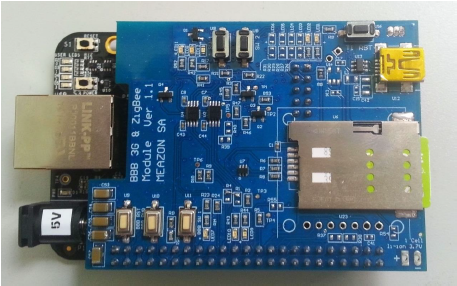
\includegraphics[width=0.7\textwidth]{eikona_24}
\caption{Μπροστινή άποψη του PCB επέκτασης, συνδεδεμένο στο BBB}\label{eik24}
\end{figure}

\begin{figure}[!hb]
\centering
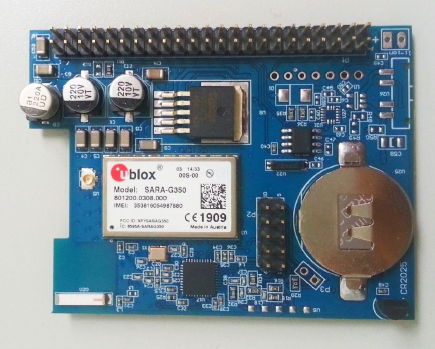
\includegraphics[width=0.7\textwidth]{eikona_25}
\caption{Πίσω άποψη του PCB επέκτασης}\label{eik25}
\end{figure}
\clearpage

\section{Εγκατάσταση Ubuntu στο BeagleBone Black}

Όπως αναφέραμε και στο προηγούμενο κεφάλαιο, το BBB έρχεται με προεγκατεστημένη τη διανομή \textenglish{Linux \AA ngstr\"om}, αλλά στη Meazon του εγκαθιστούμε μια διανομή Ubuntu. Σε υπολογιστή με λειτουργικό σύστημα Linux, στον οποίο έχουμε συνδέσει μια κάρτα micro-SD μέσω ενός card reader, με τη χρήση terminal κατεβάζουμε την έκδοση Ubuntu Saucy 13.10 από τη διεύθυνση 
\begin{code}
http://s3.armhf.com/debian/saucy/bone/ubuntu-saucy-13.10-armhf-3.8.13-bone30.img.xz
\end{code}
με την εντολή
\begin{code}
wget http://s3.armhf.com/debian/saucy/bone/ubuntu-saucy-13.10-armhf-3.8.13-bone30.img.xz
\end{code}
Αφού τελειώσει το download, επαληθεύουμε το md5 hash της εικόνας για να είμαστε σίγουροι πως δεν έχει πάθει κάποια αλλοίωση:
\begin{code}
md5sum ubuntu-saucy-13.10-armhf-3.8.13-bone30.img.xz
8173dffeaae12421a5542c3578afdd82 ubuntu-saucy-13.10-armhf-3.8.13-bone30.img.xz
\end{code}
Γινόμαστε superuser με την εντολή 
\begin{code}
sudo -i
\end{code}
επειδή οι εντολές που ακολουθούν χρειάζονται δικαιώματα superuser για να εκτελεσθούν.

Γράφουμε
\begin{code}
fdisk -l
\end{code}
για να δούμε ποιό όνομα του τύπου \slash dev\slash sdX έχει το αποθηκευτικό μέσο (κάρτα SD) που θα περιέχει το λειτουργικό. Στη δική μας περίπτωση ήταν \slash dev\slash sd1. Το επόμενο βήμα είναι να μεταβούμε στο directory που κατεβάσαμε την εικόνα και να τρέξουμε το script \emph{setup\_sdcard} με την εντολή:
\begin{code}
sudo ./setup_sdcard.sh --mmc /dev/sd1 --uboot bone_dtb
\end{code}
Αυτή η εντολή ξεκινά τη διαδικασία της αποσυμπίεσης και της αντιγραφής της εικόνας στην κάρτα, η οποία μπορεί να διαρκέσει και μέχρι μια ώρα. Μόλις αυτό τελειώσει, έχουμε αντίγραφο του λειτουργικού που θέλουμε να εγκαταστήσουμε στο BeagleBone μέσα στην κάρτα micro-SD.

Το επόμενο στάδιο είναι να φλασάρουμε την onboard κάρτα μνήμης (eMMC) του BeagleBone με την εικόνα που έχουμε στην κάρτα. Αυτό γίνεται με τα εξής βήματα:
\begin{enumerate}
\item Εισάγουμε την κάρτα στο BeagleBone. 
\item Κρατώντας το κουμπί εκκίνησης πατημένο (βρίσκεται πάνω από τη θύρα micro-SD) τροφοδοτούμε το board είτε συνδέοντάς το μέσω καλωδίου USB με τον υπολογιστή μας, είτε μέσω μετασχηματιστή. 
\item Κρατάμε το κουμπί πατημένο για περίπου 15 δευτερόλεπτα. Αυτό εξασφαλίζει πως το board θα εκκινήσει από την SD κάρτα και όχι από την εσωτερική του μνήμη. Μετά από δύο-τρία λεπτά η διαδικασία εκκίνησης έχει ολοκληρωθεί.
\item Γράφουμε στο terminal την εντολή 
\begin{code}
xz -cd ubuntu-saucy-13.10-armhf-3.8.13-bone30.img.xz > dev/mmcblk1
\end{code}
\item Όταν η διαδικασία του flash στη μνήμη eMMC (\emph{dev/mmcblk1}) ολοκληρωθεί, τα 4 LED του board θα είναι αναμμένα σταθερά.
\item Αφαιρούμε την τροφοδοσία του board.
\item Αφαιρούμε την κάρτα SD.
\end{enumerate}
Όταν ανάψουμε ξανά το board, θα εκκινήσει από την onboard κάρτα μνήμης.

%\begin{figure}
%\centering
%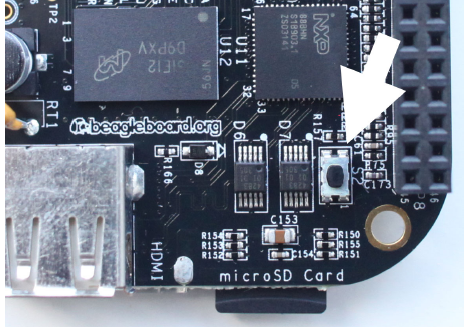
\includegraphics[width=0.8\textwidth]{eikona_boot}
%\caption{Το κουμπί εκκίνησης του BeagleBone Black}
%\end{figure}

\section{Εγκατάσταση οδηγών του BBB στον υπολογιστή}

Μετά την εγκατάσταση του λειτουργικού συστήματος στο BeagleBone Black και για τον καλύτερο χειρισμό του, θέλουμε να το συνδέσουμε τοπικά με έναν υπολογιστή μέσω της USB θύρας του. Για να αναγνωριστεί από τον υπολογιστή χρειάζεται προηγουμένως να εγκαταστήσουμε σε αυτόν τους ακόλουθους drivers. Με την εγκατάσταση των drivers o υπολογιστής επικοινωνεί με το BeagleBone Black μέσω ενός τοπικού interface, του usb0, και τη δημιουργία ενός υποδικτύου με διευθύνσεις 192.168.7.1 για τον υπολογιστή και 192.168.7.2 για το BeagleBone Black.

Σε υπολογιστή με λειτουργικό σύστημα Linux, κατεβάζουμε το αρχείο
\begin{code}
http://beagleboard.org/static/Drivers/Linux/FTDI/mkudevrule.sh
\end{code}
Το κάνουμε εκτελέσιμο με την εντολή
\begin{code}
chmod +x mkudevrule.sh
\end{code}
και το εκτελούμε με την εντολή
\begin{code}
./mkudevrule.sh
\end{code}

Σε υπολογιστή με λειτουργικό σύστημα Windows, κατεβάζουμε τους αντίστοιχους οδηγούς, ανάλογα με την έκδοση των Windows που διαθέτουμε
\begin{itemize}
\item[$\textbf{64bit:}$] \begin{code}
http://beagleboard.org/static/Drivers/Windows/BONE_D64.exe
\end{code}

\item[$\textbf{32bit:}$] \begin{code}
http://beagleboard.org/static/Drivers/Windows/BONE_DRV.exe
\end{code}
\end{itemize}

Εγκαθιστούμε τους οδηγούς βάσει των οδηγιών του προγράμματος εγκατάστασης.

\section{Επικοινωνία με το BeagleBone}

Γενικά υπάρχουν πολλοί τρόποι για να συνδεθούμε με το BeagleBone και να έχουμε πρόσβαση στη γραμμή εντολών του. Αν δεν χρησιμοποιούμε οθόνη, πληκτρολόγιο και ποντίκι, ο εναλλακτικός τρόπος χρήσης του είναι με το πρωτόκολλο SSH (Secure Shell). Σε λειτουργικό σύστημα Windows, είναι απαραίτητη η εγκατάσταση ενός τρίτου προγράμματος π.χ. putty, ενώ σε λειτουργικό Linux η σύνδεση γίνεται απλά μέσα από ένα terminal. Ο υπολογιστής που χρησιμοποιήσαμε είχε μια διανομή Linux Mint οπότε δε χρειάστηκε να εγκαταστήσουμε κάποιο επιπλέον πρόγραμμα.

Το SSH είναι ένα ασφαλές δικτυακό πρωτόκολλο το οποίο επιτρέπει τη μεταφορά δεδομένων μεταξύ δύο υπολογιστών. Το SSH κρυπτογραφεί τα δεδομένα που ανταλλάσσονται κατά τη συνεδρία και επιπλέον προσφέρει ένα ασφαλές σύστημα αναγνώρισης καθώς και άλλα χαρακτηριστικά όπως ασφαλή μεταφορά αρχείων (SSH File Transfer Protocol, SFTP).

Αν γίνεται χρήση USB καλωδίου και σύνδεση του board με τον υπολογιστή μας, τότε έχει δημιουργηθεί ένα τοπικό δίκτυο ανάμεσά τους, όπου πάντα το BeagleBone Black έχει τη διεύθυνση 192.168.7.2 και ο υπολογιστής την 192.168.7.1. Αυτός ήταν και ο τρόπος που διαλέξαμε.

Συνδέουμε το BBB με το καλώδιο USB to Mini-USB στον υπολογιστή μας και ανοίγουμε μια γραμμή εντολών (command prompt\slash terminal) όπου γράφουμε την εξής εντολή: 
\begin{code}
ssh ubuntu@192.168.7.2
\end{code} 
και μετά πατάμε enter. Θα μας ζητηθεί να εισάγουμε τον κωδικό του BeagleBone, τον οποίο έχει ορίσει η Meazon για τη συσκευή που διαθέτουμε. Mετά την επιτυχή εισαγωγή του, αποκτάμε πρόσβαση στο BeagleBone(σχ~\ref{eik27}).

\begin{figure}[!ht]
\centering
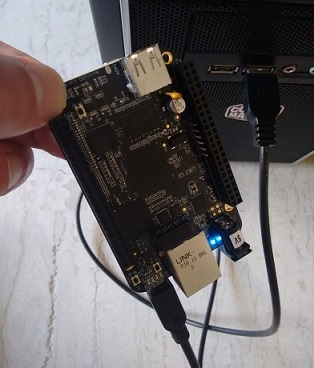
\includegraphics[scale=0.72]{eikona_26}
\caption{Σύνδεση του BeagleBone στον υπολογιστή}
\end{figure}

\begin{figure}[t]
\centering
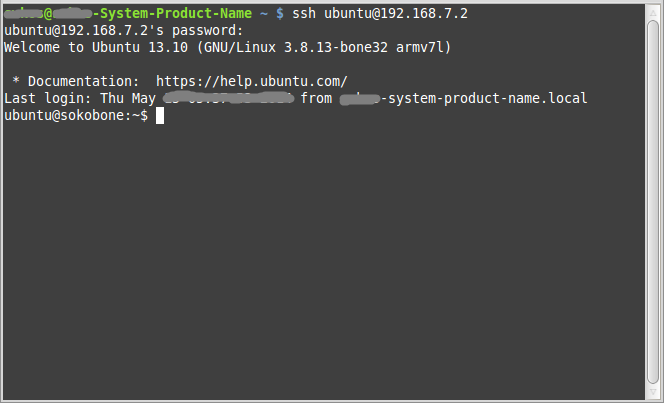
\includegraphics[width=0.97\textwidth]{eikona_27}
\caption{Επιτυχής σύνδεση στο σύστημα του BeagleBone}\label{eik27}
\end{figure}

Σε περίπτωση που δε χρησιμοποιείται καλώδιο USB για τη σύνδεση του BeagleBone Black με υπολογιστή, μπορεί να αποκτηθεί πρόσβαση μέσω δικτύου. Για να γίνει γνωστή η διεύθυνση ip του BeagleBone Black θα πρέπει να χρησιμοποιηθεί ένα πρόγραμμα σάρωσης δικτύου. Στα αποτελέσματα σάρωσης θα αναφέρεται ο κατασκευαστής θύρας δικτύου που στην προκειμένη περίπτωση θα είναι η ``Texas Instruments''.

Το όνομα που είχαμε δώσει στη συσκευή που χρησιμοποιήσαμε ήταν sokobone, για αυτό και στο path που φαίνεται στο terminal βλέπουμε να γράφει \verb+ubuntu@sokobone:~$+ όταν συνδεόμαστε σε αυτήν.

\section[Βιβλιοθήκη για έλεγχο GPIOs]{Εγκατάσταση βιβλιοθήκης σε Python για έλεγχο των GPIO pins}

Για την επεξεργασία των GPIO pins του BeagleBone θα χρειαστεί η εγκατάσταση των βιβλιοθηκών για τη γλώσσα Python. Οι βιβλιοθήκες αυτές μας δίνουν την δυνατότητα να ορίσουμε τα pin σαν εισόδους ή εξόδους, να μιλήσουμε στα διάφορα interfaces που μας παρέχει το BeagleBone, όπως η σειριακή και το I$^2$C. Πριν την εγκατάσταση των βιβλιοθηκών θα πρέπει να εγκαταστήσουμε κάποια εργαλεία που είναι απαραίτητα για την Python όπως το setuptools. Το setuptools είναι ένα πακέτο βιβλιοθήκης για προγραμματιστικές διαδικασίες, σχεδιασμένο να οργανώνει τα Python projects ενσωματώνοντας τα βασικά εργαλεία βιβλιοθηκών. Η εγκατάσταση γίνεται με την παρακάτω εντολή.
\begin{code}
sudo apt-get install build-essential python-dev python-setuptools python-pip python-smbus –y
\end{code}

Η εντολή για την εγκατάσταση της βιβλιοθήκης για τα GPIO pins είναι η
\begin{code}
sudo pipinstallAdafruit_BBIO
\end{code}

Για τον έλεγχο της σωστής εγκατάστασης, θα πρέπει να εκτελεσθεί η επόμενη εντολή
\begin{code}
sudo python -c "import Adafruit_BBIO.GPIO as GPIO; print GPIO"
\end{code}
και να εκτυπώσει τα παρακάτω:
\begin{code}
<module 'Adafruit_BBIO.GPIO' from '/usr/local/lib/python2.7/dist-packages Adafruit_BBIO/GPIO.so'>
\end{code}

Ένας εναλλακτικός τρόπος εγκατάστασης σε περίπτωση που δε λειτουργήσει ο πρώτος λόγω ασυμβατότητας εκδόσεων είναι ο εξής:
\begin{itemize}
\item[-] Κατέβασμα του πηγαίου κώδικα από την πλατφόρμα GitHub με την εντολή \begin{code}
git clone git://github.com/adafruit/adafruit-beaglebone-io-python.git
\end{code}
\item[-] Μετάβαση στον αντίστοιχο φάκελο \begin{code}
cd adafruit-beaglebone-io-python
\end{code}
\item[-] Εκτέλεση του αρχείου εγκατάστασης \begin{code}
sudo python setup.py install
\end{code}
\end{itemize}
Στη συνέχεια πρέπει να αφαιρεθεί ο πηγαίος κώδικας σβήνοντας τον κατάλογο:
\begin{code}
cd ..
sudo rm -rf adafruit-beaglebone-io-python
\end{code}



\section{Επεξεργασία αρχείων του BeagleBone}

Προτού κάνουμε οποιαδήποτε μεταβολή στα αρχεία του BeagleBone για να κάνουμε την πλακέτα επέκτασης ένα GPRS router, θα πρέπει να σιγουρευτούμε πως δεν ``τρέχει'' η διαδικασία (daemon) που στέλνει μηνύματα ZigBee μεταξύ των μετρητικών συσκευών και του BeagleBone. Ο daemon αυτός λέγεται zigway και είναι γραμμένος σε γλώσσα Pyhton. Για να βρούμε το ID της διαδικασίας γράφουμε την εντολή 
\begin{code}
ps -ae|grep python
\end{code}
στο terminal, βλέπουμε μετά ποιο είναι το ID της και για να την τερματίσουμε γράφουμε στο terminal 
\begin{code}
sudo kill -9 #
\end{code}
όπου αντικαθιστούμε το \# με τον αριθμό του ID της. Για να επαληθεύσουμε πως τερματίστηκε η διεργασία, ξαναγράφουμε την πρώτη εντολή και αν η διεργασία έχει όντως τερματισθεί, το terminal δε θα μας δώσει κάποια απάντηση. Η διαδικασία αυτή φαίνεται στο σχ.~\ref{eik28}.

\begin{figure}[!b]
\centering
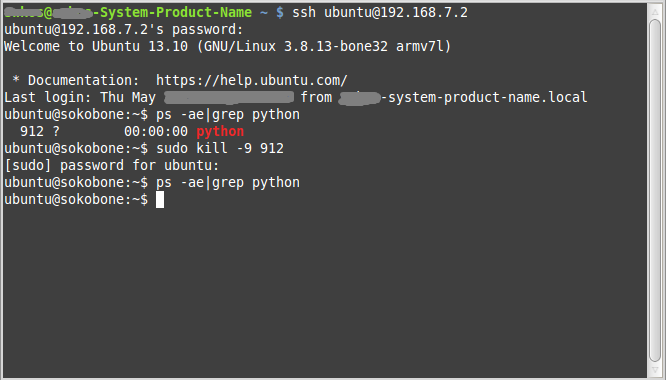
\includegraphics[scale=0.8]{eikona_28}
\caption{Ανίχνευση και τερματισμός του daemon}\label{eik28}
\end{figure}

Η πλακέτα επέκτασης συνδέεται με pins στη μία από τις δύο σειρές υποδοχών επέκτασης (Cape Expansion Headers) που διαθέτει το Beaglebone, αυτήν που αναφέρεται ως P9. Η αρίθμηση όλων των expansion headers και για τις δύο σειρές που διαθέτει το BeagleBone φαίνεται στο σχ.~\ref{eik22}.

Το U270 της u-blox είναι ένα module που προσφέρει υψηλής ταχύτητας συνδεσιμότητα μέσω δικτύων κινητής τηλεφωνίας. Το module μπορεί να υποστηρίξει ταχύτητες της τάξης των 7.2MB/s για το download και 5.76MB/s για το upload. Είναι σχεδιασμένο με στόχο την χαμηλή κατανάλωση, πράγμα που το κάνει ιδανικό για τη χρήση σε μικρές συσκευές. Η χρήση του γίνεται με AT Commands μέσω κάποιου terminal όπως το Minicom ή το Cutecom.

Το U270 έχει τα εξής χαρακτηριστικά:
\begin{itemize}
\item UMTS\slash HSPA 850\slash 1900 και 900\slash 1200 MHz
	\begin{itemize}
	\item 3GPP Release 7
	\item 5.76 MB\slash upload, 7.2 Mb\slash s download
	\end{itemize}
\item GSM 850\slash 1900 και 900\slash 1200 MHz
\item GPRS Class 12, CS1-CS4 μέχρι 86.5 kb\slash s
\item CSD GSM max 9.6 kb\slash s
\item UMTS max 64 kb\slash s
\item SMS MT\slash MO PDU \slash{} Text mode
\item Voice HR\slash FR\slash EFR\slash AMR\slash AMR-WB
\item Audio-over-USB
\item Echo cancellation and noise reduction
\end{itemize}

Για να επικοινωνήσει το U270 με το BeagleBone, χρησιμοποιείται η σειριακή θύρα UART1. Για το λόγο αυτό θα πρέπει να ενεργοποιηθεί το συγκεκριμένο interface μέσω του λειτουργικού συστήματος Linux του BeagleBone. Πρέπει να επεξεργασθεί το αρχείο ``\texttt{uEnv.txt}'' με κάποιον text editor (εδώ χρησιμοποιήθηκε ο vim), το οποίο βρίσκεται στον κατάλογο ``\texttt{\slash boot\slash uboot}''. Το αρχείο αυτό είναι ένα αρχείο κειμένου που χρησιμοποιείται από τον bootloader του BeagleBone και διαμορφώνει την εκκίνησή(boot) του, το οποίο μπορούμε να χρησιμοποιήσουμε για να περάσουμε παραμέτρους στον πυρήνα(kernel) του Linux του Beaglebone. Ο βασικός Linux bootloader που χρησιμοποιείται στο BBB λέγεται \textenglish{\emph{Das U-Boot}(Universal Bootloader)}.

Στη συνέχεια, θα πρέπει να αναφέρουμε τα interfaces που θέλουμε να ενεργοποιηθούν. Για παράδειγμα, για να ενεργοποιήσουμε τα UART1 και UART4, θα πρέπει να γράψουμε στο αρχείο: 
\begin{code}
optargs=quiet drm.debug=7 capemgr.enable_partno=BB-UART1,BB-UART4
\end{code}

Για να ενεργοποιηθεί η θύρα που θέλουμε, θα πρέπει μετά την αλλαγή που κάναμε στο αρχείο να επανεκκινήσουμε το BeagleBone. Αυτό γίνεται με την εντολή \verb+sudo reboot+. Στο παρακάτω σχήμα φαίνεται η συγκεκριμένη διαδικασία.

\begin{figure}[!hb]
\centering
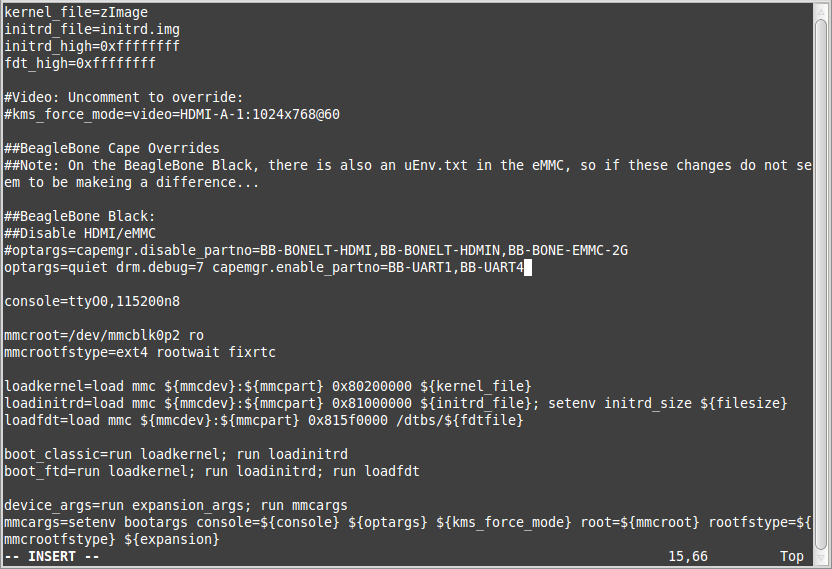
\includegraphics[scale=0.6]{eikona_30}
\caption{Επεξεργασία του uEnv.txt}\label{eik30}
\end{figure}

Στον πίνακα~\ref{pinakas2} σημειώνουμε σε ποιό pin header του BeagleBone αντιστοιχεί η κάθε σειριακή θύρα UART. Συνολικά το BeagleBone έχει 4 τέτοιες θύρες, από τις οποίες μόνο η UART0 είναι ενεργοποιημένη από προεπιλογή. Για να ενεργοποιήσουμε οποιαδήποτε άλλη, πρέπει να ακολουθήσουμε τη διαδικασία που αναφέρθηκε προηγουμένως. Με την εντολή 
\begin{code}
ls -l /dev/tty0*
\end{code}
μας δίνει σαν απάντηση ποιές σειριακές θύρες είναι ενεργοποιημένες. Μετά την επανεκκίνηση του BeagleBone χρησιμοποιούμε το πρόγραμμα Cutecom για να σετάρουμε τις σειριακές θύρες που ενεργοποιήσαμε, με το baud rate που θέλουμε.

\begin{figure}[!h]
\centering
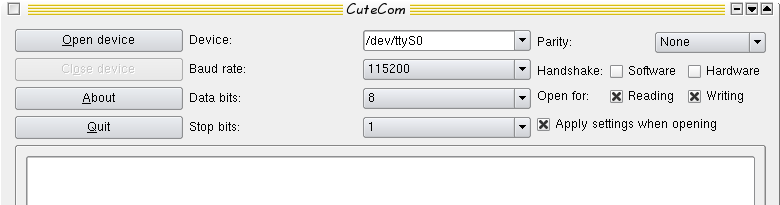
\includegraphics[width=0.9\textwidth]{eikona_29}
\caption{Δείγμα ενός παραθύρου του προγράμματος Cutecom}\label{eik29}
\end{figure}

%\begin{table}[t]
%\centering
%\begin{tabular}{|c|c|c|c|c|c|}
%\hline
% & RX & TX & CTS & RTS & Συσκευή\\ \hline
%UART0 & J1\_4 & J1\_5 & & & \slash dev\slash tty00\\ \hline
%UART1 & P9\_26 & P9\_24 & P9\_20 & P9\_19 & \slash dev\slash tty01\\ \hline
%UART2 & P9\_22 & P9\_21 & P8\_37 & P8\_38 & \slash dev\slash tty02\\ \hline
%UART3 &  & P9\_42 & P8\_36 & P8\_34 & \slash dev\slash tty03\\ \hline
%UART4 & P9\_11 & P9\_13 & P8\_35 & P8\_33 & \slash dev\slash tty04\\ \hline
%UART5 & P8\_38 & P8\_37 & P8\_31 & P8\_32 & \slash dev\slash tty05\\ 
%\hline
%\end{tabular}
%\caption{Αντιστοιχία UARTs και pin headers}\label{eik31}
%\end{table}

Το επόμενο αρχείο που θα πρέπει να επεξεργαστούμε είναι \phantom{a}το \mbox{``\texttt{\slash etc\slash ppp\slash peers\slash provider}''}. Το αρχείο αυτό δηλώνει ποιο αρχείο περιέχει τις AT εντολές, το σειριακό interface που είναι συνδεδεμένο το module καθώς και το Baud rate της σύνδεσης. Οι εντολές που θα πρέπει να γράψουμε στο αρχείο είναι
\begin{code}
connect "/user/bin/chat -v -f /etc/chatscripts/pap -T *99#"
/dev/tty01
115200
\end{code}

Το πεδίο tty01 είναι το UART1 και 115200 είναι το baud rate της σύνδεσης. Ο αριθμός *99\#{} που βάλαμε είναι για το δίκτυο κινητής τηλεφωνίας COSMOTE. Εάν χρησιμοποιήσουμε άλλο πάροχο θα πρέπει να αλλάξουμε το συγκεκριμένο πεδίο. Στο σχ.~\ref{eik31} φαίνεται η επεξεργασία του αρχείου.
\clearpage
\begin{figure}[!h]
\centering
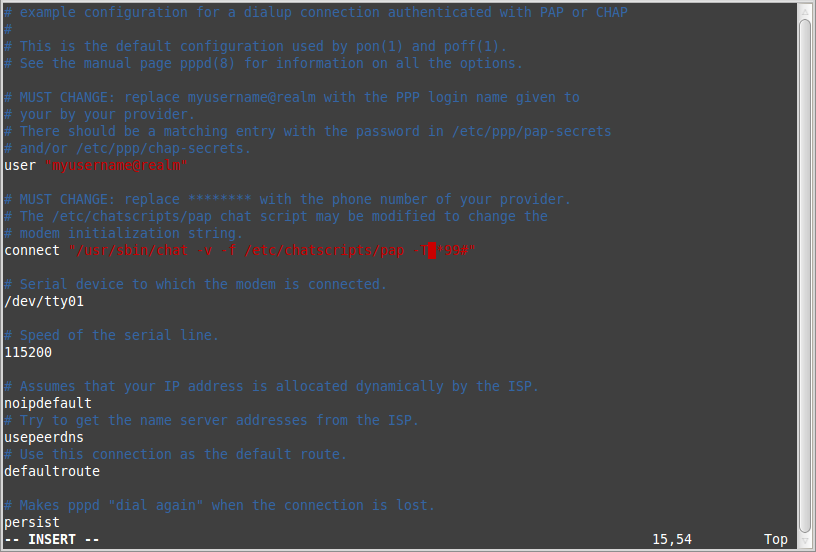
\includegraphics[scale=0.55]{eikona_31}
\caption{Το αρχείο ``\slash etc\slash ppp\slash peers\slash provider''}\label{eik31}
\end{figure}

Το τελευταίο αρχείο που πρέπει να επεξεργαστούμε για να κάνουμε το module να λειτουργήσει ως GPRS modem είναι το ``\texttt{\slash etc\slash chatscripts\slash pap}''. To πακέτο αυτό περιέχει τις AT εντολές που θα δημιουργήσουν τη σύνδεση. Οι εντολές που γράφουμε φαίνονται στο σχ.~\ref{eik32} και είναι οι εξής

\begin{code}
""			AT
OK			AT+CMEE=2
OK			AT+COPS=0
OK			AT+CGDCONT=1,"IP","INTERNET"
OK			AT+CGACT=1,1
OK			ATD*99#
CONNECT
\end{code}

Το ΑΤ+CMEE=2 είναι ένας δείκτης για τη λειτουργία και τα σφάλματα του module. To AT+COPS=0 αναγκάζει το module να επιλέξει και να εγγραφεί σε ένα δίκτυο. Με το ΑΤ+CGDCONT=1,``IP'',``INTERNET'' συμπληρώνει τα στοιχεία APN που χρειάζεται ο πάροχος κινητής τηλεφωνίας. Με το ΑΤ+CGACT=1,1 ενεργοποιείται το Packet Data Protocol. Στη συνέχεια γίνεται η σύνδεση που δημιουργεί ένα PPP interface στο Linux το οποίο παίρνει ένα μοναδικό process id και τέλος μια μοναδική real IP διεύθυνση.

\begin{figure}[!h]
\centering
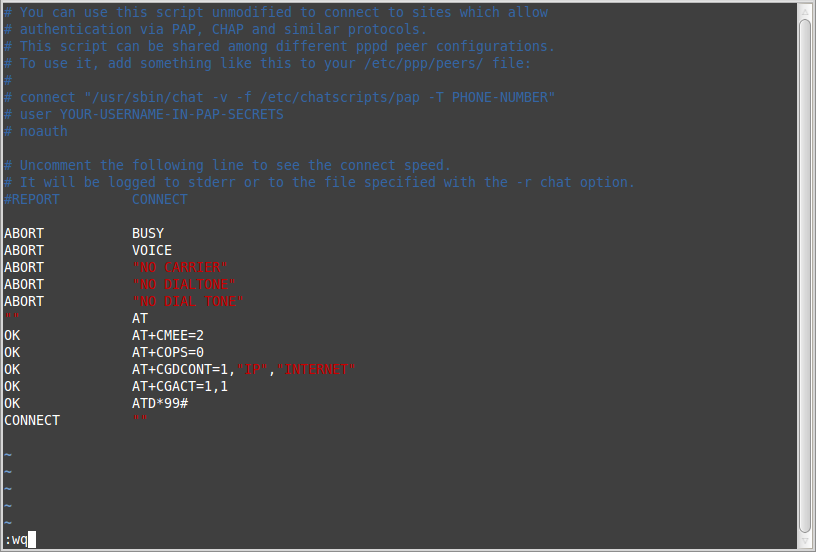
\includegraphics[scale=0.55]{eikona_32}
\caption{Το αρχείο ``\slash etc\slash chatscripts\slash pap''}\label{eik32}
\end{figure}

Για να μπορέσει το module να χρησιμοποιηθεί ως modem θα πρέπει να εγκατασταθεί ένα πακέτο το οποίο θα αυτοματοποιήσει κάποιες διαδικασίες. Το πακέτο αυτό ονομάζεται psmisc και το εγκαθιστούμε γράφοντας στο terminal την εντολή 
\begin{code}
sudo apt-get install psmisc
\end{code}
Με το πακέτο αυτό μπορούμε να εκτελέσουμε ή να σταματήσουμε ένα αρχείο με το μπλοκ των AT εντολών που επιθυμούμε, με στόχο την δημιουργία σύνδεσης στο internet.

Αφού λοιπόν εγκαταστήσουμε το πακέτο και έχουμε επεξεργαστεί τα αρχεία με τις σωστές ρυθμίσεις, η εντολή για την έναρξη του interface είναι 
\begin{code}
pppd call provider
\end{code} 
και για τη λήξη του είναι 
\begin{code}
sudo killall pppd
\end{code}
Μπορούμε να παρακολουθούμε μηνύματα κατά τη λειτουργία του interface με την εντολή 
\begin{code}
plog
\end{code}

Στα παραπάνω σχήματα φαίνεται η δημιουργημένη σύνδεση καθώς και το αποτέλεσμα της εντολής plog.

\begin{figure}
\centering
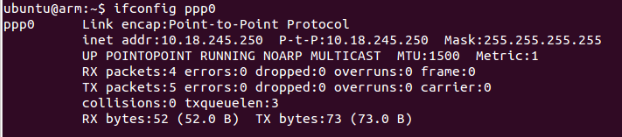
\includegraphics[scale=0.8]{eikona_33}
\caption{Η σύνδεση μέσω GPRS}
\end{figure}

\begin{figure}
\centering
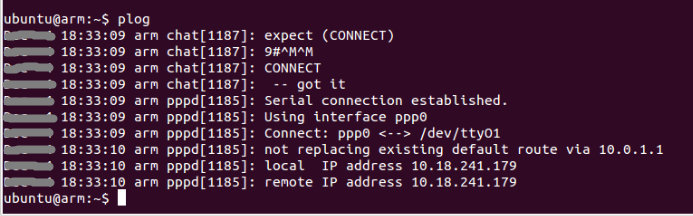
\includegraphics[scale=0.75]{eikona_34}
\caption{Μηνύματα μετά την εντολή plog}
\end{figure}

Μετά τη δημιουργία της GPRS σύνδεσης μπορούμε να εκκινήσουμε ξανά την εφαρμογή, καλώντας τον daemon με την εντολή 
\begin{code}
sudo service zigway start
\end{code}
Από εκεί και πέρα αναλαμβάνει η εφαρμογή της Meazon\label{app} να στέλνει τα μετρητικά δεδομένα στο cloud, καθώς και τον έλεγχο των μετρητικών συσκευών(σχ.\ref{eik35})

\begin{figure}[!ht]
\centering
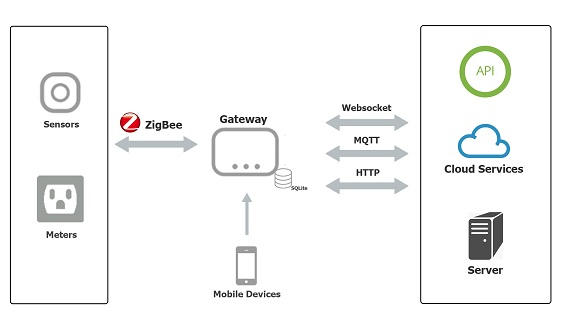
\includegraphics[scale=0.7]{eikona_35}
\caption[Τα διάφορα στάδια της υπηρεσίας της Meazon]{Τα διάφορα στάδια της υπηρεσίας της Meazon\cite{meazon}}\label{eik35}
\end{figure}

Τέλος, πρέπει να σημειώσουμε πως η κάρτα SIM που θα χρησιμοποιηθεί, θα πρέπει να έχει απενεργοποιημένη την αίτηση κωδικού PIN, γιατί δε γίνεται να βάζουμε τον κωδικό αυτόματα μέσω του BeagleBone. Αυτό μπορεί να γίνει εύκολα αν τοποθετήσουμε τη SIM σε ένα κινητό τηλέφωνο πριν την εισάγουμε στο expansion board, και με τις κατάλληλες ρυθμίσεις να απενεργοποιήσουμε το συγκεκριμένο χαρακτηριστικό.

\begin{figure}[!hb]
\centering
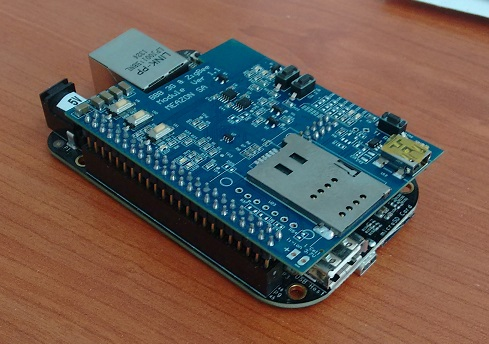
\includegraphics[scale=0.5]{eikona_36}
\caption{Το BeagleBone μαζί με την πλακέτα επέκτασης}\label{eik36}
\end{figure}
\clearpage
\section{Χρήση του Real Time Clock DS1307}

Το DS1307 είναι ένα Real Time Clock (RTC) χαμηλής κατανάλωσης, δυαδικά κωδικοποιημένο με δεκαδικό ρολόι\slash ημερολόγιο συν 56 bytes ΝV SRAM τροφοδοτούμενη από μπαταρία. Το ρολόι παρέχει πληροφορίες για δευτερόλεπτα, λεπτά, ώρες, μέρες, μήνες και χρόνια. Στο τέλος του μήνα υπολογίζει αυτόματα τους μήνες με λιγότερες από 31 ημέρες καθώς και τα χρόνια με περισσότερες μέρες. Επίσης λειτουργεί σε φορμάτ 12 και 24 ωρών. Ο DS1307 έχει εγκατεστημένο έναν αισθητήρα που ``καταλαβαίνει'' πότε δεν τροφοδοτείται με ρεύμα και αυτόματα ενεργοποιεί την εφεδρική μπαταρία. Η λειτουργία με μπαταρία μπορεί να διαρκέσει για μήνες.

Για να λειτουργήσει το RTC πρέπει να ενεργοποιηθεί o σειριακός δίαυλος I$^2$C. Ο I$^2$C Χρησιμοποιεί μόνο δύο καλώδια, τα οποία είναι αμφίδρομης κατεύθυνσης: Τα SCL και SDA. Η γραμμή SCL είναι η γραμμή ρολογιού, ενώ η SDA είναι η γραμμή δεδομένων. Οι γραμμές αυτές συνδέονται σε όλες τις συσκευές στο δίαυλο I$^2$C. Προφανώς, εκτός από τα παραπάνω καλώδια, απαιτείται και ένα τρίτο καλώδιο, το οποίο είναι η γείωση (GND) ή 0V. Επίσης μπορεί να υπάρχει και ένα τέταρτο καλώδιο το οποίo είναι η γραμμή τροφοδοσίας, με την οποία τροφοδοτούνται με ισχύ οι διάφορες συσκευές που υπάρχουν στο δίκτυο. Τυπικές τάσεις που χρησιμοποιούνται στο δίαυλο είναι τα +5V ή 3,3V, αν και επιτρέπονται συστήματα με διαφορετικές τάσεις (συνήθως στην περιοχή από 1,2V-5,5V).

Το interface ενεργοποιείται με την εντολή
\begin{code}
echo BB-I2C1 > /sys/devices/bone_capemgr.9/slots
\end{code}
και βλέπουμε ότι έχει ενεργοποιηθεί με
\begin{code}
ls -l /sys/bus/i2c/devices/i2c-*
\end{code}

Το BeagleBone Black δεν διαθέτει από μόνο του RTC, για το λόγο αυτό ενημερώνεται για την ώρα από servers στο ίντερνετ. Την πρώτη φορά που θα ρυθμιστεί το εξωτερικό RTC το board θα πρέπει να έχει σωστή ώρα.

Για να είναι εφικτή η επικοινωνία με το RTC
\begin{code}
echo ds1307 0x68 > /sys/class/i2c-adapter/i2c-1/new_device
\end{code}

Πρέπει το BeagleBone να ενημερωθεί με τη σωστή ώρα
\begin{code}
ntpdate -b -s -u pool.ntp.org
\end{code}

Εγγραφή ώρας στο RTC
\begin{code}
Hwclock -w -f /dev/rtc1
\end{code}

Με τη χρήση του RTC εξασφαλίζουμε την ορθότητα των χρονικών στιγμών που αναφέρονται οι μετρήσεις που έρχονται από τις μετρητικές συσκευές, ακόμα και σε περίπτωση που υπάρξει απώλεια τροφοδοσίας στο BeagleBone για οποιονδήποτε λόγο.

\section{Τηλεφωνική κλήση και SMS}

Πέρα από την παροχή σύνδεσης στο διαδίκτυο, η πλακέτα επέκτασης θα μπορούσε να χρησιμοποιηθεί για να ειδοποιείται ο χρήστης όταν το BeagleBone δεν έχει σύνδεση στο internet. Η ειδοποίηση θα γίνεται με SMS ή με τηλεφωνική κλήση μέσα από το δίκτυο κινητής τηλεφωνίας. Αυτό απαιτεί την κάρτα SIM μιας εταιρείας κινητής τηλεφωνίας που να είναι εγγεγραμμένη στο δίκτυο.

Για την τηλεφωνική κλήση χρειάζεται να γίνει ενεργοποίηση της υπηρεσίας και στη συνέχεια να κληθεί ο αριθμός του αποδέκτη.
\begin{code}
AT+CLIP=1
ATD+3930012345678;
\end{code}

Για την αποστολή SMS μηνύματος πρέπει να επιλεχθεί ο αριθμός του αποδέκτη καθώς και το κείμενο που θα αποσταλεί.
\begin{code}
AT+CMGS=''+3930012345678''
SMS TEXT MESSAGE
0123456789<CTRL-Z>
\end{code}

\section{Αποστολή - Χρήση μετρητικών δεδομένων}

Όπως αναφέραμε και στο τέλος της ενότητας~\ref{app}(σελ.~\pageref{app}), μόλις δημιουργηθεί η σύνδεση με το διαδίκτυο, αναλαμβάνει η εφαρμογή που ``τρέχει'' στο BeagleBone για την αποστολή και διαχείρηση των δεδομένων των μετρητικών συσκευών. Πώς όμως χρησιμοποιούνται αυτά τα δεδομένα και πού τα στέλνει η εφαρμογή;

Ο daemon που ``τρέχει'' στο BeagleBone, είναι προγραμματισμένος να ``ρωτά'' τις μετρητικές συσκευές που ανήκουν στο ZigBee δίκτυό του και αυτές του ``απαντούν'' με τις μετρήσεις τους ανά διαστήματα του ενός λεπτού. Μετά, ανά διαστήματα των 15 λεπτών, στέλνει μέσω Διαδικτύου τα μετρητικά δεδομένα που έχει συγκεντρώσει, στην υπηρεσία Cloud της Meazon όπου και αποθηκεύονται. Έτσι κρατείται αναλυτικό ιστορικό του καθενός μετρητή ξεχωριστά, που παρέχει πληροφορία για την κατανάλωση σε ενέργεια, για τις τιμές του ρεύματος, της θερμοκρασίας, τη συχνότητα του δικτύου κ.ά., που μετρήθηκαν σε συγκεκριμένες χρονικές στιγμές.

Η Meazon έχει αναπτύξει μια web εφαρμογή ονόματι Meazon Izy, στην οποία μπορεί να συνδέεται όποιος έχει προμηθευτεί BeagleBone και μετρητικές συσκευές και να βλέπει το λεπτομερές ιστορικό των μετρήσεων ενέργειας που κατέγραψαν οι μετρητές του υπό όρους μέσης κατανάλωσης σε διαστήματα 5 λεπτών. Πέρα από το ιστορικό, μπορεί να βλέπει και τα δεδομένα που επιστρέφουν οι μετρητές σε πραγματικό χρόνο και μπορεί να το κάνει από οποιοδήποτε μέρος κι αν βρίσκεται, αρκεί να έχει πρόσβαση στο Internet. Ακόμα, μέσω της εφαρμογής έχει τη δυνατότητα να ενεργοποιεί\slash απενεργοποιεί ξεχωριστά το ενσωματωμένο ρελέ του κάθε μετρητή τον οποίο έχει συνδέσει στο δίκτυο ZigBee που έχει δημιουργήσει το BeagleBone, επιλέγοντας με αυτόν τον τρόπο από απόσταση το αν θα βρίσκονται σε λειτουργία ή όχι οι ηλεκτρικές συσκευές που έχει συνδέσει στους μετρητές. Τέλος, η εφαρμογή της Meazon δίνει και τη δυνατότητα για προγραμματισμό (scheduling) στο χρήστη, ώστε να ορίζει το πότε θα γίνονται αυτόματα ορισμένες ενέργειες (π.χ. άνοιγμα\slash κλείσιμο εξωτερικών φώτων).

\begin{figure}[!ht]
\centering
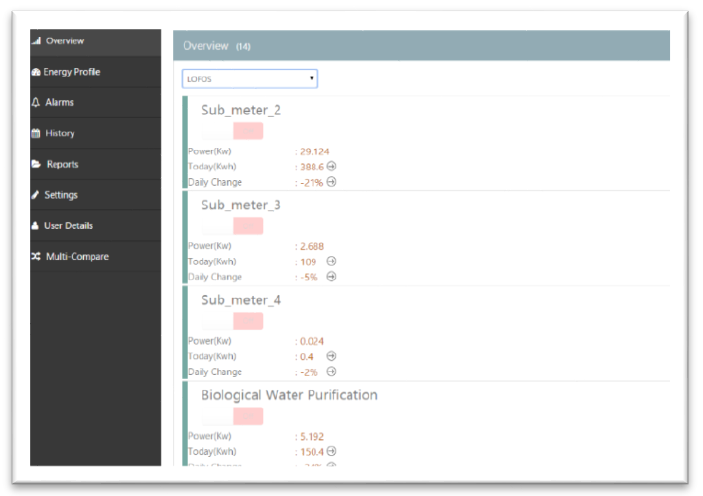
\includegraphics[width=0.78\textwidth]{eikona_37}
\caption[Στιγμιότυπο της εφαρμογής]{Στιγμιότυπο της εφαρμογής\cite{meazon}}\label{eik37}
\end{figure}

Μετά από λεπτομερή εξέταση των δεδομένων αυτών, συγκρίνοντας με την προηγούμενη ημέρα, εβδομάδα ή μήνα για αντίστοιχες περιόδους, μπορεί να εξαχθεί το ενεργειακό προφίλ του καταναλωτή στον οποίον αφορούν οι μετρητικές συσκευές. Έτσι, μπορούμε να δούμε την τάση και την εξέλιξη που έχει το φορτίο του στο χρόνο και να αναλάβει ανάλογες δράσεις ώστε να περιορίσει την κατανάλωση ενέργειας που έχει.

Στο σχ.~\ref{eik37} δείχνουμε ένα στιγμιότυπο της εφαρμογής Meazon Izy, η οποία πέρα από web εφαρμογή, υπάρχει διαθέσιμη και ως εφαρμογή για smartphone, δίνοντας στο χρήστη τη δυνατότητα να κάνει αυτά που περιγράφηκαν παραπάνω και από το κινητό του τηλέφωνο.

\section{Παραδείγματα Χρήσης}

Το BeagleBone μαζί με την πλακέτα επέκτασης μπορεί να χρησιμοποιηθεί σε μέρη όπου η ενσύρματη πρόσβαση στο διαδίκτυο δεν είναι εφικτή, έτσι ώστε σε συνδυασμό με τις μετρητικές συσκευές της Meazon να έχουμε τη δυνατότητα να μετρούμε και να ελέγχουμε ηλεκτρικές συσκευές και εγκαταστάσεις που βρίσκονται σε τέτοιες περιοχές.

Ένα πιθανό σενάριο εφαρμογής θα μπορούσε να είναι κάποιο αντλιοστάσιο που βρίσκεται σε μια αγροτική περιοχή και χρησιμοποιείται για την άρδευση καλλιεργήσιμων εκτάσεων. Εγκαθιστώντας το BeagleBone μαζί με έναν τριφασικό μετρητή (συνήθως τέτοιες αντλίες απαιτούν τριφασική παροχή) θα μπορούσε κάποιος αγρότης από την άνεση του σπιτιού του να ελέγχει το πότε θα λειτουργεί η αντλία που παρέχει το νερό στις καλλιέργειές του, χωρίς να χρειάζεται η φυσική του παρουσία στο χώρο του αντλιοστασίου, κερδίζοντας έτσι χρόνο. Επίσης, μέσω των μετρήσεων θα μπορεί να κάνει μια μελλοντική εκτίμηση για το κόστος της ενέργειας που θα κληθεί να πληρώσει στον πάροχο ηλεκτρικής ενέργειας, ανάλογα με τις ώρες που θα λειτουργεί το αντλιοστάσιο. Έτσι, θα μπορεί να βρίσκει τη χρυσή τομή ανάμεσα στο πόσο επιπλέον κέρδος περιμένει να του προσφέρει η καλλιέργειά του λόγω περισσότερης ποσότητας νερού και στο κόστος της ενέργειας που θα χρειαστεί να πληρώσει για αυτή.

Άλλη περίπτωση που θα μπορούσε να χρησιμοποιηθεί το BeagleBone με το expansion board θα ήταν σε περιπτώσεις που θέλουμε να ελέγξουμε κάποια εγκατάσταση όπου δεν υπάρχει ήδη ενεργοποιημένη κάποια σύνδεση στο διαδίκτυο μέσω παρόχου σταθερής τηλεφωνίας. Η αποστολή των μετρητικών δεδομένων και των εντολών ελέγχου δεν απαιτεί μεγάλο όγκο δεδομένων, μερικές εκατοντάδες MB το μήνα είναι αρκετά, επομένως αντί για τη δημιουργία μιας καινούριας σύνδεσης για Internet μέσω σταθερής τηλεφωνίας, θα μπορούσε κανείς να εξυπηρετηθεί με πολύ μικρότερο κόστος, αγοράζοντας ένα πλάνο παροχής MB με κάποιο καρτοκινητό.

Ένα σενάριο είναι η περίπτωση που κάποιος διαθέτει ένα εξοχικό σπίτι στο οποίο έχει σταθερό τηλέφωνο αλλά δεν έχει υπογράψει συμβόλαιο παροχής Internet, καθώς το σπίτι δε χρησιμοποιείται όλη τη χρονιά. Με την επιλογή ενός πλάνου για παροχή Internet μέσω καρτοκινητού θα μπορεί να ελέγχει και να μετρά την κατανάλωση ενέργειας που έχει το σπίτι του στις περιόδους που το χρησιμοποιεί και ο ίδιος επιθυμεί. Ακόμη, θα μπορεί να ενεργοποιεί ηλεκτρικές συσκευές του σπιτιού, π.χ. τον ηλεκτρικό θερμοσίφωνα επιστρέφοντας από την παραλία το καλοκαίρι ή ενεργοποιήση του καυστήρα του καλοριφέρ το χειμώνα όταν ξεκινά για το ταξίδι προς το εξοχικό, ώστε να τις βρίσκει έτοιμες όταν φτάσει και να κερδίζει χρόνο.


\section{Συμπεράσματα}

Με την παρούσα διπλωματική καταφέραμε να δώσουμε τη δυνατότητα στο BeagleBone να συνδεθεί στο διαδίκτυο μέσω του δικτύου κινητής τηλεφωνίας και έτσι να μπορέσουμε να ελέγξουμε τις μετρητικές μας συσκευές από απόσταση μέσω Internet. Με αυτόν τον τρόπο κάνουμε <<έξυπνο>> το μέρος όπου έχουμε εγκαταστήσει τις συσκευές αυτές, και έτσι η ηλεκτρική εγκατάσταση αυτή μπορεί να ενταχθεί εύκολα σε ένα Έξυπνο Δίκτυο Ενέργειας. Η υλοποίηση αυτή ανήκει στο τμήμα των πελατών ενός έξυπνου δικτύου σύμφωνα με το μοντέλο που ορίστηκε από το NIST\cite{21}, καθώς αφορά και χρησιμοποιείται από τον τελικό χρήστη.% και όχι από την εταιρεία παροχής ηλεκτρικής ενέργειας.

Μέσω της παρακολούθησης και ανάλυσης του ιστορικού της κατανάλωσης ενέργειας, που επιτυγχάνεται με τη χρήση της κατάλληλης εφαρμογής που παρέχει η Meazon, μπορεί να εξαχθεί το ενεργειακό προφίλ του καταναλωτή και να δει ο ίδιος σε ποιά σημεία μπορεί να επέμβει ώστε να εξοικονομήσει ενέργεια. Ακόμα, ο χρήστης μπορεί να κάνει πρόβλεψη για το ποσό της ενέργειας που θα καταναλώσει σε διάστημα συγκεκριμένου χρόνου, οπότε θα μπορεί να κάνει πιο εύκολα τον οικονομικό του προγραμματισμό. Επίσης, με τη χρήση των μετρητικών συσκευών μπορεί να ελέγχει την κατάσταση λειτουργίας των ηλεκτρικών συσκευών που έχει συνδέσει σε αυτές, δηλαδή το αν λειτουργούν ή όχι (on\slash of\mbox{}f state) και μπορεί να προγραμματίζει από απόσταση συγκεκριμένες λειτουργίες ώστε να γίνονται αυτόματα (π.χ. έλεγχος φωτιστικών, συστήματος ποτισμού).

Με τη λύση της παροχής σύνδεσης στο διαδίκτυο μέσω GPRS, απαλλαχθήκαμε από την ανάγκη ύπαρξης σταθερής ευρυζωνικής σύνδεσης για την εγκατάσταση του BeagleBone και των μετρητικών συσκευών. Έτσι, μπορούμε ουσιαστικά να εγκαταστήσουμε ένα τέτοιο σύστημα οπουδήποτε υπάρχει κάλυψη από κινητή τηλεφωνία και να έχουμε τη δυνατότητα να ελέγχουμε μια εγκατάσταση με ηλεκτρικές συσκευές από την άνεση του σπιτιού μας. Με αυτό τον τρόπο μπορούμε να συντελέσουμε στο να ενσωματωθούν περισσότερα τμήματα του υπάρχοντος ηλεκτρικού δικτύου, σε ένα <<Έξυπνο Δίκτυο>> που θα είναι μετρήσιμο και ελέγξιμο, με όλα τα οικονομικά καθώς και περιβαλλοντικά οφέλη που αυτό σημαίνει, λόγω της εξοικονόμησης ενέργειας.



%\begin{figure}[!h]
%\centering
%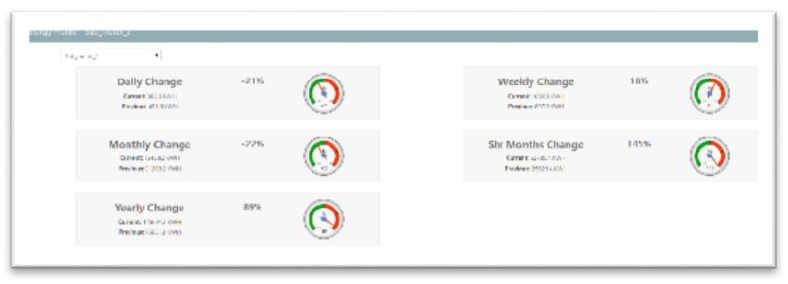
\includegraphics[width=0.95\textwidth]{eikona_38}
%\caption[Ενεργειακό προφίλ καταναλωτή]{Ενεργειακό προφίλ καταναλωτή\cite{meazon}}\label{eik38}
%\end{figure}




\clearpage


%%%%%%%%%%%%%%%%%%%% PORNH VIVLIOGRAFIA %%%%%%%%%%%%%%%%%%
%\addcontentsline{toc}{chapter}{Βιβλιογραφία}
\begin{thebibliography}{99}

\bibitem{fang}
F. Li, W. Qiao, H. Sun, H. Wan, J. Wang, Y. Xia, Z. Xu, P. Zhang, ``Smart Transmission Grid: Vision and Framework'', IEEE Transactions on Smart Grid, vol. 1, no. 2, Sep. 2010.

\bibitem{39}
``A Reliability Perspective of the Smart Grid'', Khosrow Moslehi and Ranjit Kumar. IEEE Transactions on Smart Grid June 2010.

\bibitem{40}
``Annual report on US wind power installation, cost and performance trends'', 2007 Energy Ef\mbox{}f\mbox{}iciency and Renewable Energy, U.S Department of Energy, 2008.

\bibitem{9}
``Οικονομική λειτουργία συστημάτων ηλεκτρικής ενέργειας'', Μπακιρτζής Αναστάσιος, εκδ. ΖΗΤΗ, 1998.

\bibitem{41}
``The ef\mbox{}fects of integrating wind power on transmission system planning, reliability and operations'', report on phase 2: System performance evaluation New York State Energy Research and Development Authority, Albany, NY, 2005.

\bibitem{4}
N. I. of Technology-Calicut, ``An Advanced Metering Infrastructure for Future Electricity Networks'', pp. 1–16.

\bibitem{42}
``Waiting for the sunrise (solar energy forecast)'', The Economist, May 1990.

\bibitem{6}
ENISA, ``Smart Grid Security - Annex I - General Concepts and Dependencies with ICT'', 2012.

\bibitem{11}
X. Li and I. Lille, ``Securing Smart Grid : Cyber Attacks , Countermeasures , and Challenges'', no. August, pp. 38–45, 2012.

\bibitem{12}
T. Flick, ``Securing the Smart Grid: Next Generation Power Grid Security''. ELSEVIER, 2011.

\bibitem{13}
Minnesota Power, ``About Electricity'', 2012.

\bibitem{15}
D. Y. Xi Yang, Satyajayant Misra, Guoliang Xue, ``Smart Grid – The New and Improved Power Grid : A Survey'', 2011.

\bibitem{16}
E. Commision and Brussels, ``Smart Grids: from innovation to deployment'', COM(2011) 202 final, 2011.

\bibitem{17}
EU Commission Task Force for Smart Grids, ``Functionalities of smart grids and smart meters Final Deliverable'', December, pp. 1–69, 2010.

\bibitem{18}
NIST and Smart Grid Co-ordination Group, ``White paper on standardization of Smart Grids''.

\bibitem{19}
C. Boutin, ``U.S., Europe Collaborating on Smart Grid Standards Development''. NIST Tech Beat, 2011.

\bibitem{zwtou}
Ευφροσύνη Θ. Ζώτου, ``Σύγχρονες Τεχνολογίες Πρόσβασης και Διαδικτύου σε Έξυπνα Δίκτυα (Smart Grids)'', 2012.

\bibitem{20}
CEN CENELEC ETSI, ``Final report Standards for Smart Grids'', May, 2011.

\bibitem{21}
U.S. Department of Commerce, ``NIST Special Publication 1108 NIST Framework and Roadmap for Smart Grid Interoperability Standards, Release 1.0'', 2010.

\bibitem{22}
C. Lima, ``Enabling a Smarter Grid'', September, 2010.

\bibitem{pyramid}
http://www.ecofactor.com

\bibitem{iot}
Executive Summary: ``The Internet of Things'', ITU Internet Reports, Nov. 2005.

\bibitem{cisco}
http://blogs.cisco.com/sp/from-internet-of-things-to-web-of-things


\bibitem{43}
``Solar energy industry forecast: Perspectives on U.S. solar market trajectory'', Solar Energy Technologies Program, U.S. Department of Energy,2008.

\bibitem{44}
Executive summary: ``Assessment of parabolic trough and power tower solar technology cost and performance forecasts'', National Renewable Energy Laboratory, 2003.

\bibitem{schneider}
http://www2.schneider-electric.com

\bibitem{45}
``Harnessing the power of demand - How ISOs and RTOs are integrating demand response into wholesale electricity markets'', Markets Committee of the ISO\slash RTO Council, 2007.

\bibitem{biz}
http://meazon.com/products/bizyplug/

\bibitem{din}
http://meazon.com/products/dinrail-basic/

\bibitem{zig1}
ZigBee Specif\mbox{}ication, Jan. 2008, διαθέσιμο στο www.zigbee.org

\bibitem{ieee}
IEEE 802.15.4: Wireless Medium Access Control (MAC) and Physical Layer (PHY) Specif\mbox{}ications for Low-Rate Wireless Personal Area Networks (WPANs), Sept. 2006.

\bibitem{zigbee}
http://rowebots.com/wireless\_protocols/zigbee

\bibitem{wlan}
IEEE 802.11: Wireless LAN Medium Access Control (MAC) and Physical Layer (PHY) Specif\mbox{}ications.

\bibitem{zigarrows}
S. Farahani, ``ZigBee Wireless Networks and Transceivers'', Elsevier Ltd., 2008.

\bibitem{zig2}
http://www.icpdas.com

\bibitem{guti}
J. Gutierrez, ``Low-Rate Wireless Personal Area Networks'', John Wiley \& Sons, 2011

\bibitem{OSI}
Open Systems Interconnection Basic Reference Model: The Basic Model, ISO/IEC 7498-1:1994.

\bibitem{46}
D. Molloy, ``Exploring BeagleBone: Tools and Techniques for Building with Embedded Linux'', John Wiley \& Sons, 2015.

\bibitem{47}
M. Richardson, ``Getting Started with BeagleBone'', Maker Media, 2014.

\bibitem{48}
www.beagleboard.org

\bibitem{arduino}
www.arduino.cc

\bibitem{raspberry}
https://www.sparkfun.com

\bibitem{bifferboard}
http://robosavvy.com

\bibitem{parallela}
https://www.parallella.org

\bibitem{meazon}
http://meazon.com

\bibitem{sara}
http://www.u-blox.com/en/wireless-modules/gsm-gprs-modules/sara-gsm-module-family.html

\bibitem{49}
https://www.u-blox.com/images/downloads/Product\_Docs/EVK-G3x\_GettingStarted\_\%28UBX-13001792\%29.pdf

\bibitem{50}
http://www.u-blox.com/images/downloads/Product\_Docs/u-blox-ATCommands\_Manual\_\%28UBX-13002752\%29.pdf

\end{thebibliography}
\clearpage

\pagenumbering{gobble}
\phantom{grrr}
\begin{figure}[b]
\centering

\includegraphics[scale=0.1]{telepitelous}
\end{figure}

\end{document}

%%%%%% Watermark gia to telos %%%%
\clearpage

\pagenumbering{gobble}
\phantom{grrr}
\begin{figure}[b]
\centering

\includegraphics[scale=0.1]{telepitelous}
\end{figure}
